\documentclass[12pt, a4paper, oneside]{memoir}
%oneside for soft copy
%twoside for hard final copy
\setlrmargins{4.3cm}{*}{*}
\checkandfixthelayout
%\documentclass[12pt, a4paper, oldfontcommands]{memoir}
%\documentclass[12pt, a4paper]{report}

\usepackage{amsmath}
\usepackage{amsthm}
\usepackage{amssymb}
\usepackage{amsbsy}
\usepackage{graphicx}
\usepackage[outdir=./]{epstopdf}
\usepackage[round]{natbib} 
\usepackage{url}
\usepackage{subcaption}
\usepackage{hyperref}
\usepackage{hyphenat}
\usepackage{pdfpages}
\usepackage{MnSymbol} %udots
\usepackage{afterpage} %\afterpage{\clearpage}
\usepackage{siunitx} %for measurements
\usepackage[figuresright]{rotating}
\usepackage{multirow} %for multirow tables
\usepackage{mathtools} %multlined
\usepackage{longtable}
\usepackage{bibentry}

\setcounter{tocdepth}{2}
\setcounter{secnumdepth}{2}

\let\footruleskip\undefined
\usepackage{fancyhdr}
\fancypagestyle{plain}{%
\fancyhf{}% clears all header and footer fields
\fancyhead[LE,RO]{\thepage}%
\renewcommand{\headrulewidth}{0pt}%
\renewcommand{\footrulewidth}{0pt}}

\DeclareMathOperator{\expfamily}{ExpFamily}
\DeclareMathOperator{\expectation}{\mathbb{E}}
\DeclareMathOperator{\variance}{\mathbb{V}ar}
\DeclareMathOperator{\cov}{\mathbb{C}ov}
\DeclareMathOperator{\corr}{\mathbb{C}orr}
\DeclareMathOperator{\bernoulli}{Bernoulli}
\DeclareMathOperator{\betaDist}{Beta}
\DeclareMathOperator{\dirichlet}{Dir}
\DeclareMathOperator{\bin}{Bin}
\DeclareMathOperator{\MN}{Multinomial}
\DeclareMathOperator{\prob}{\mathbb{P}}
\DeclareMathOperator{\trace}{Tr}
\DeclareMathOperator{\normal}{N}
\DeclareMathOperator{\gammaDist}{Gamma}
\DeclareMathOperator{\poisson}{Poisson}
\DeclareMathOperator{\CPoisson}{CP\Gamma}
\DeclareMathOperator*{\argmax}{argmax}

\newcommand{\RSS}{\mathrm{RSS}}
\newcommand{\euler}{\mathrm{e}}
\newcommand{\diff}{\mathrm{d}}
\newcommand{\T}{^\textup{T}}
\newcommand{\BIC}{\mathrm{BIC}}
\newcommand{\AIC}{\mathrm{AIC}}

\newcommand{\subSize}{0.49\textwidth}
\newcommand{\mainSize}{0.8\textwidth}

\newcommand{\vect}[1]{\mathbf{#1}}
\newcommand{\vectGreek}[1]{\boldsymbol{#1}}
\newcommand{\matr}[1]{\mathsf{#1}}

\newcommand{\addNumber}[1]{\protect\input{#1}\unskip}
\newcommand{\inputNumber}[1]{\protect\input{#1}\unskip}

\DeclareSIUnit\pixel{px}
\DeclareSIUnit\adu{ADU}
\OnehalfSpacing*
\begin{document}\sloppy

\begin{titlingpage}
\centering
{\LARGE Characterisation of Computed Tomography Noise in Projection Space with Applications to Additive Manufacturing \par}
\vspace{1cm}
{\Large Sherman Edea Lo\par}
{\Large Doctor of Philosophy in Statistics\par}
\vfill
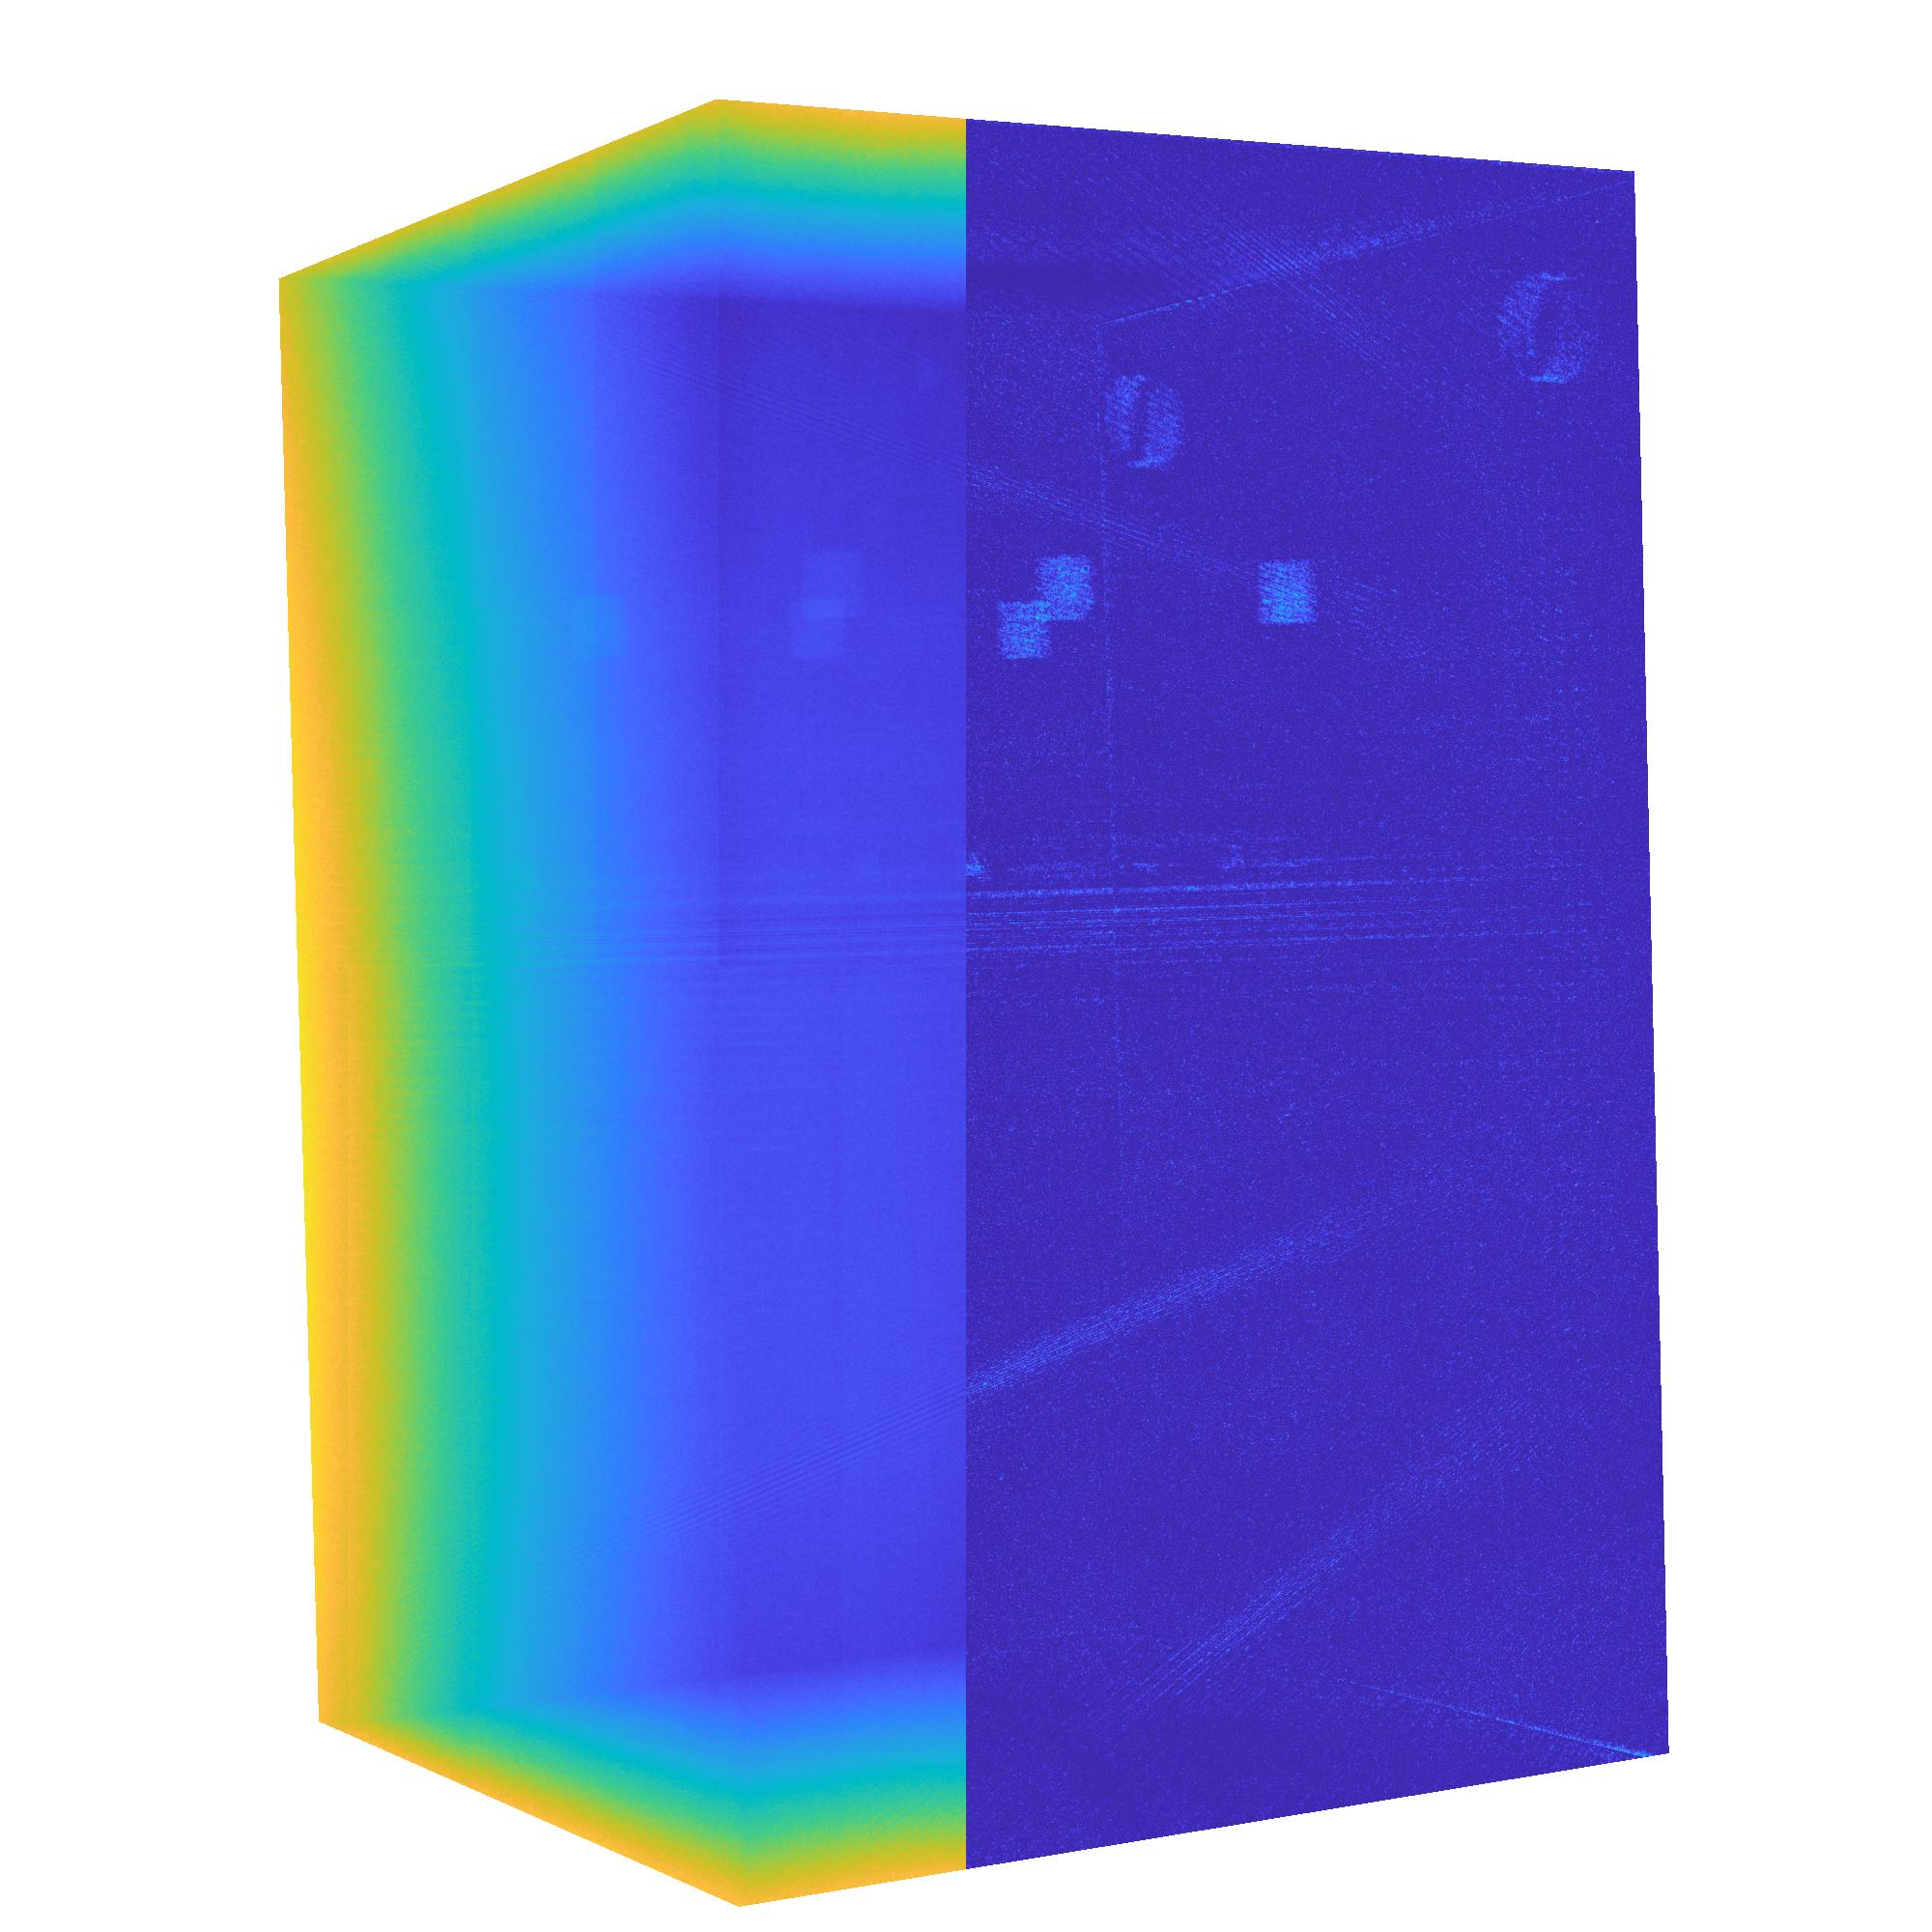
\includegraphics[width = 0.75\textwidth]{../figures/frontCover.jpg}
\vfill
{\Large University of Warwick\par}
{\Large Department of Statistics\par}
{\Large September 2019\par}
\end{titlingpage}


\frontmatter

\cleardoublepage
\tableofcontents*
\cleardoublepage
\listoffigures
\cleardoublepage
\listoftables

\chapter{Acknowledgements}
I would like to thank my supervisors Julia Brettschneider and Tom Nichols for their guidance throughout my PhD. I would also like to thank my calibrators who are part of the Inside-Out group, in Warwick Statistics, Clair Barnes, Wilfred Kendall and Audrey Kueh, and the Warwick Manufacturing Group, Greg Gibbons, Jay Warnett and Mark Williams.

This work is funded by the EPSRC and MRC Centre for Doctoral Training in Next Generation Statistical Science: The Oxford-Warwick Statistics Programme (EP/L016710/1). I would like to thank my cohort for the friendship and collaboration during the programme: Nathan Cunningham, Giuseppe di Benedetto, Beniamino Hadj-Amar, Jack Jewson, Ella Kaye, Leon Law, Kaspar M\"{a}rtens, Marcin Mider, Xenia Miscouridou, Paul Vanetti, Andi Wang.

\chapter{Declaration}
This thesis is submitted to the University of Warwick in support of my application for the degree of Doctor of Philosophy. It has been composed by myself and has not been submitted in any previous application for any degree.

The work presented (including data generated and data analysis) was carried out by the author except in the cases outlined below:
\begin{itemize}
  \item The fabrication, x-ray computed tomography acquisition and simulation of test samples were done by Greg Gibbons and Jay Warnett, from the Warwick Manufacturing Group, as part of Inside-out: Statistical methods for Computed Tomography validation of complex structures in Additive Layer Manufacturing funded by EPSRC (EP/K031066/1).
\end{itemize}

Parts of this thesis is anticipated to be published by the author:
\begin{itemize}
  \item\nobibliography*\bibentry{lo2019detection}
\end{itemize}

\chapter{Abstract}
X-ray computed tomography can be used for defect detection in additive manufacturing. Typically, several x-ray projections of the product at hundreds of angles are used to reconstruct the object in 3D to look for any defects. The process can be time-consuming. This thesis aims to investigate if it is possible to conduct defect detection from a single projection to speed up the process. An additive manufacturing test sample was created with voids to see if they can be detected.

The uncertainty of the projection was modelled using a compound Poisson distribution. This arises from x-ray photon arrivals being a Poisson process and each photon has random energy. This results in a linear relationship between the mean and variance of the grey values in the projection. Fitting of the compound Poisson distribution using the expectation-maximisation algorithm was unsuccessful due to identifiability issues with the model. Instead, a gamma-distributed generalised linear model was fitted onto sample variance-mean data and used for variance prediction to quantify the uncertainty.

Software, called \emph{aRTist}, was used to simulate the projection and compared with the experimental projection in the face of uncertainty by treating each pixel as a hypothesis test. To overcome the imperfections of the simulation, the empirical null filter was used to cater for model misspecification so that sensible inference was achieved. This was done by locally normalising the test statistics using the mode. Voids with diameters in the order of millimetres were detectable.

This thesis is a contribution to real-time quality control in additive manufacturing.

\newpage

\mainmatter

\chapter{Introduction}

In the field of engineering, additive manufacturing is an emerging technology and has uses in producing bespoke products. Because it is a new form of technology, the process is not well understood and tolerances are not as precise as other forms of manufacturing. As a result, there exist methods for quality control of additive manufactured products. Typically, this is done using x-ray computed tomography and requires hundreds of x-ray projections, making this a slow process.

The main aim of this thesis is to investigate if it is possible to speed up the quality control process of additive manufactured products by using only a few x-ray projections. By using fewer x-ray projections, uncertainty is introduced. This can be tackled by using statistics because it enables the sensible handling of uncertainty from sources of error such as random error and systematic error.

The analysis was done by comparing the experimental projection with a simulated projection to look for areas with disagreement in the face of uncertainty. Random error can arise from how x-ray photons are produced in an x-ray tube and how they interact with the additive manufactured product and the x-ray detector. This was modelled by using the compound Poisson distribution. Incorrect simulation of the projection contribute to systematic error and this was corrected using the empirical null filter. These sources of error were considered in the comparison of the projections with the use of hypothesis testing.

The front cover shows the before and after of the statistical analysis. The left-hand side shows an x-ray projection of an additive manufactured cuboid. Its edges appeared curved due to spot and panel effects and this can be fixed using shading correction. The right-hand side shows the $p$-values of the resulting inference. Lighter colours show evidence of a defect and they successfully highlighted voids put in there purposefully.

In Chapter \ref{chapter1}, x-ray computed tomography and additive manufacturing is reviewed. Sources of error were investigated and see how they were handled. In Chapter \ref{chapter2}, a test sample was additively manufactured and the chapter describes how experimental x-ray projections were obtained. Shading correction is explained here and it was used to remove sources of systematic error in the projections. In Chapter \ref{chapter3}, the compound Poisson distribution is studied so that it can be used to model the detection of x-rays. In Chapter \ref{chapter4}, the uncertainty in the projection was quantified using the variance and generalised linear models were used to predict it. In Chapter \ref{chapter5}, novel statistical techniques were developed and implemented to look for defects in the test sample in the face of uncertainty. This was done by comparing the experimental projection with a simulated projection and looking for any disagreement. The empirical null filter was used to cater for any model misspecification so that sensible conclusions were made. The thesis ends with an evaluation in Chapter \ref{chapter6}.

The results presented in this thesis can be reproduced using the source code in the \emph{GitHub} repository \url{https://github.com/shermanlo77/oxwasp_phd}.

\chapter{Literature Review}
\label{chapter1}
One of the first methods of additive manufacturing (AM) is stereolithography \citep{kodama1981automatic, hull1986apparatus, 3d2019our} which involves the curing of a photosensitive resin using an ultraviolet laser. The technology has evolved and AM is capable of manufacturing objects with complicated internal and external geometries, some examples are shown in Figure \ref{fig:literature_3dprint}. However, there is a need for product inspection and in particular assessing the quality of the internal structures.

\begin{figure}
  \centering
  
\includegraphics[width=0.9\textwidth]{../figures/literatureReview/literature_3dprint.png}
  \caption{Examples of additive manufactured parts: a) lattice structure, b) toy, c) chain, d) model of a facial implant, e) spanner, f) ratchet mechanism, g) toy, h) series of rotatable gears, i) lattice structure. Republished with permission of Springer New York, from \cite{gibson2010additive}; permission conveyed through Copyright
Clearance Center, Inc.}
  \label{fig:literature_3dprint}
\end{figure}

Imaging using x-rays \citep{rontgen1896on} have been used in the medical field. In x-ray computed tomography \citep{cormack1973reconstruction, hounsfield1973computerized, hounsfield1980computed}, the patient has an x-ray image taken at multiple angles. These x-ray images are used to reconstruct what was taken in 3D to make a diagnostic.

X-ray computed tomography (XCT) can be used as a non-destructive test for AM products. Various reviews on AM exist such as \cite{kruth1991material, kruth1998progress, pham1998comparison, gibson2010additive, wong2012review, ngo2018additive}. For XCT used in manufacturing, there are \cite{cantatore2011introduction, kruth2011computed, sun2012overview}. \cite{thompson2016x} reviewed the applications of XCT on AM.

In this chapter, AM is reviewed followed by XCT. The latest research for the use of XCT on AM is reviewed at the end of the chapter.

\section{Additive Manufacturing}

Loosely, AM involves solidifying material onto a moving platform so that the object is manufactured layer by layer. Typically, this is a slow and expensive method compared to destructive methods such as computer numerical control (CNC) machining for example. An advantage of AM is that the setup cost is low, in particular, destructive methods require planning and setting up various apparatus before the manufacturing stage \citep{gibson2010additive}. This makes it suitable to manufacture bespoke items which achieves the goals of AM's predecessor called rapid prototyping \citep{kruth1991material}.

Various AM technologies were invented during the advancement of AM. Because of this, there are various applications of AM, for example in medical and biomedical sciences \citep{kang20163d, kourra2018computed}, engineering \citep{cooper2015design}, food engineering \citep{godoi20163d} and art \citep{ornes2013mathematics, grossman2019bathsheba}.

\subsection{Additive Manufacturing Technologies}

The different AM technologies can be classified based on the apparatus, for example, liquid-based or powder-based, and/or on the method of manufacturing, for example, point by point or layer by layer \citep{kruth1991material}. The liquid-based AM technologies presented here are stereolithography \citep{kodama1981automatic, hull1986apparatus, 3d2019our} and fused deposition modelling \citep{crump1991fused, crump1992apparatus, stratasys2019what}. The following powder-based technologies are presented here: 3D printing \citep{sachs1990three}, selective laser sintering \citep{deckard1989method, dtm1990the, 3d2019our}, electron beam melting \citep{larsson2004arrangement, arcam2019history}, laser engineered net shaping \citep{atwood1998laser}. Illustrations of these technologies are shown in Figure \ref{fig:literature_technologies}.

\begin{figure}
  \centering
  \centerline{
    \begin{subfigure}[b]{0.59\textwidth}
      
\includegraphics[width=\textwidth]{../figures/literatureReview/literature_technologies_stl.png}
      \caption{Stereolithography}
    \end{subfigure}
    \begin{subfigure}[b]{0.39\textwidth}
      
\includegraphics[width=\textwidth]{../figures/literatureReview/literature_technologies_fdm.png}
      \caption{Fused deposition modelling}
    \end{subfigure}
  }
  \centerline{
    \begin{subfigure}[b]{0.7\textwidth}
      
\includegraphics[width=\textwidth]{../figures/literatureReview/literature_technologies_3dp.png}
      \caption{3D printing}
    \end{subfigure}
  }
  \centerline{
    \begin{subfigure}[b]{0.7\textwidth}
      
\includegraphics[width=\textwidth]{../figures/literatureReview/literature_technologies_laser.png}
      \caption{Selective laser sintering}
    \end{subfigure}
  }
  \caption{Diagrams of various AM technologies. Reprinted from \cite{wang20173d}\textsuperscript{\textcopyright}, with permission from Elsevier.}
  \label{fig:literature_technologies}
\end{figure}

Stereolithography is a liquid-based AM technology. It consists of a container containing a liquid photo-hardening monomer or polymer as well as a piston and platform which holds and moves the manufactured product up and down. A laser with a specific wavelength, typically \SIrange{300}{400}{\nano\metre} \citep{kodama1981automatic}, is emitted onto a point of the surface of the liquid and solidifies. The laser is controlled by a computer to solidify specific parts of the liquid surface. The platform is lowered and the cycle repeats, manufacturing the object layer by layer. Laser absorption happens a few tenths of a millimetre which corresponds to the thickness of each layer \citep{kruth1991material, pham1998comparison}.

Fused deposition modelling is another liquid-based AM technology. A jetting head, or nozzle, deposit the molten material onto a platform or on top of the previous layer. The material is usually plastic in the form of a thin filament. It is heated to just above its melting points, typically \SI{1}{\degreeCelsius} \citep{crump1992apparatus}, so that it cools down within \SI{0.1}{\second} \citep{kruth1991material}. The platform moves, and controlled by a computer, in the $xy$ plane, or left to right and front to back, to produce a layer. The jetting head can move in the $z$-axis, or up and down, to manufacture the next layer. In the original patent by \cite{crump1992apparatus}, the thickness can be as thin as 0.000\,1 inches (\SI{0.003}{\milli\metre}).

3D printing is a powder-based AM technology. A jetting head deposits a binding agent in droplets onto a bed of powder of ceramic, metal or polymer. The binding agent is cured via evaporation or heating which glues the powder particles together. The jetting head can move in the $xy$-plane and the object is manufactured layer by layer by moving the platform in the $z$-axis and renewing the powder using a roller. The binding agent must have a low viscosity so it can be deposited and may also be charged so that it can be deflected using an electric field for precise deposition \citep{sachs1990three}. The thickness of each layer is determined by the size of the droplets of the binding agent, which can be as small as \SI{15}{\micro\metre} in diameter \citep{sachs1990three}. \cite{sachs1990three} reported a tolerance of 0.001 inches (\SI{0.03}{\milli\metre}).

Selective laser sintering, electron beam melting and laser engineered net shaping are powder-based AM technology. Selective laser sintering is similar to 3D printing, but instead, a laser is used to sinter or fuse the powder particles in a chamber heated just below the melting point of the material \citep{wong2012review}. Various materials such as metals and plastics can be used \citep{wong2012review}. Electron beam melting is similar, but instead of a laser, an electron beam is used. This is done in a high vacuum chamber to avoid oxidation \citep{wong2012review}. In laser engineered net shaping, a powder bed is not used; the powder is deposited on the desired location and then melted using a laser, as shown in Figure \ref{fig:literature_lens}. This is a popular method to manufacture metal objects \citep{gibson2010additive}.

\begin{figure}
  \centering
  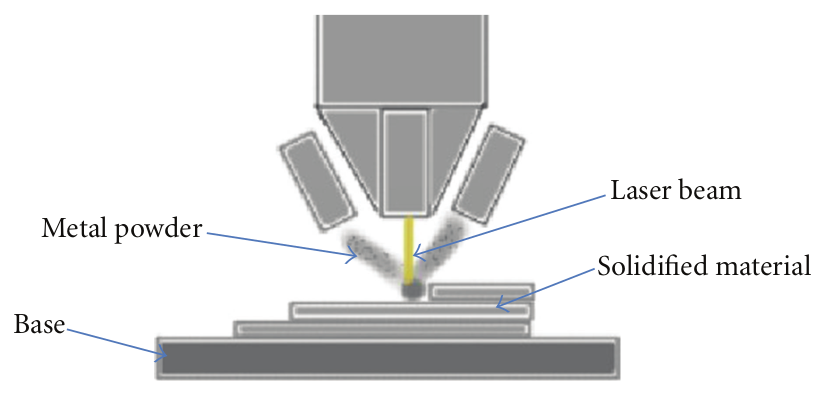
\includegraphics[width=0.7\textwidth]{../figures/literatureReview/literature_lens.png}
  \caption{Laser engineered net shaping. Reprinted from \citep{wong2012review} under the CC BY 3.0 license.}
  \label{fig:literature_lens}
\end{figure}

There are many more AM technologies but they can be found in numerous review literature. A comparison of the mentioned AM technologies available at the time was done by \cite{pham1998comparison, kim2008benchmark}. Factors such as material cost, mechanical properties and the resolution of the manufacturing were considered. There are also safety aspects to assess, for example, powder in powder-based methods can escape into the environment and the liquid used in stereolithography is toxic, sticky and has spilling risk \citep{kim2008benchmark}. This makes fused deposition modelling a popular choice and can be used in an office environment \citep{ngo2018additive}.

The strength of the manufactured object varies from geometry to geometry but also from direction to direction. Because the manufactured object is made layer by layer, the strength varies if the load was applied in the building direction (vertical) or the scanning direction (horizontal) \citep{kim2008benchmark}. Experimental results have shown that fused deposition modelling has superior strength in the scanning direction but weak in the building direction \citep{kim2008benchmark}.

The strongest manufacturing methods were found to be powder-based methods and stereolithography, however, they are slow and material costs are high \citep{kim2008benchmark}. Fused deposition modelling has low costs and high speeds but suffers from weak mechanical properties \citep{ngo2018additive}.

The materials available for each AM technology varies. The materials used in stereolithography is limited because of the use of liquids with photo-hardening properties \citep{ngo2018additive}. Fused deposition modelling is limited to plastics \citep{ngo2018additive}. Selective laser sintering and laser engineered net shaping can manufacture objects using metals such as aluminium alloys, steel, titanium and titanium alloys \citep{herzog2016additive}.

\subsection{Pre/Post Processing}

The blueprint of the object to be manufactured is called a computer-aided design (CAD) model. For it to be processed by an AM apparatus, the CAD model is converted to an STL file \citep{3d1989sterolithography, 3d2019what} which represent surfaces by a series of triangles, an example is shown in Figure \ref{fig:literature_stl}. STL stands for stereolithography but could also be called standard tessellation language \citep{wong2012review}. Some accuracy is lost here as the surface of the CAD model is represented approximately by triangles \citep{gibson2010additive}. The STL file is then sliced into layers \citep{jamieson1995direct, vatani2009enhanced} so that the AM apparatus knows what to build for each layer.

\begin{figure}
  \centering
  
\includegraphics[width=0.9\textwidth]{../figures/literatureReview/literature_stl.png}
  \caption{An example of a CAD model (left) converted to a STL file (right). Republished with permission of Springer New York, from \cite{gibson2010additive}; permission conveyed through Copyright
Clearance Center, Inc.}
  \label{fig:literature_stl}
\end{figure}

When the AM object is manufactured, post-processing techniques can be done at this stage. For example, sanding may be done to smooth the surfaces \citep{gibson2010additive}. The manufactured object may be inspected for pores or defects by comparing the x-ray projection of the object with the CAD model \citep{lee2015compliance, villarraga2015assessing, kim2016inspection}.

As with any apparatus, regular maintenance is required \citep{bell2014maintaining}.

\subsection{Defects and Quality Control}

There are various discontinuities in AM. In fused deposition modelling, a staircase effect on the surface of the product arises from poor slicing methods of the CAD model \citep{weeren1995quality}. Internal voids can be formed due to insufficient material flow \citep{weeren1995quality}. Other factors which can cause defects include misalignment of the platform or nozzle, depletion of material and lack of adhesion due to low temperatures \citep{gunaydin2018common}.

There are also problems in the manufacturing of metal parts \citep{everton2016review}, for example, gas can become trapped during the manufacturing process forming gas pores in the manufactured object \citep{thijs2010study, tammas2015xct}. These gas pores can be \SIrange{5}{20}{\micro\metre} in diameter \citep{everton2016review}.

Layers may not fuse and form elongated pores. This can be fixed by increasing the energy of the beam but increasing it too much will cause evaporation of the AM part \citep{mumtaz2008high}. These pores can be \SIrange{50}{500}{\micro\metre} in size \citep{everton2016review} and can be observed using a scanning electron microscope as shown in Figure \ref{fig:literature_pores}.

Low wetting ability of the melt pool can cause balling which is where the sintered powder has poor contact on the existing layer causing spherical particles to form on the surface of the AM part \citep{li2012balling, gu2009balling}. The spherical particles can vary in size of \SIrange{10}{500}{\micro\metre} \citep{li2012balling}. The balling effect can be reduced by ensuring low oxygen content in the environment \citep{niu1999instability} and using higher energy beams \citep{gu2009balling}. Some examples are shown in Figure \ref{fig:literature_balling} using an electron scanning microscope.

Cracks can form due to extreme temperature changes and gradients \citep{mercelis2006residual, zaeh2010investigations}.

\begin{figure}
  \centering
  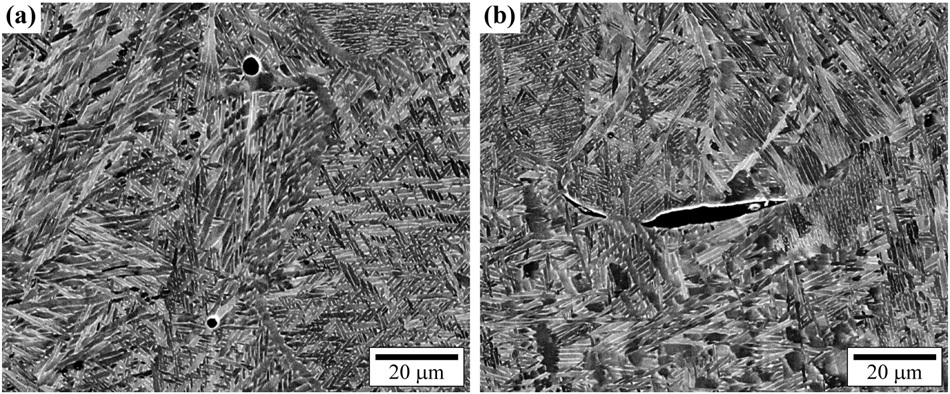
\includegraphics[width=0.99\textwidth]{../figures/literatureReview/literature_pores.png}
  \caption{A scanning electron microscope image of a) pores and b) elongated pores from an electron beam melting manufactured object. Reprinted from \cite{tammas2015xct} under the CC BY 4.0 license.}
  \label{fig:literature_pores}
\end{figure}

\begin{figure}
  \centering
  
\includegraphics[width=0.7\textwidth]{../figures/literatureReview/literature_balling.png}
  \caption{A scanning electron microscope image of balling on a selective laser melting manufactured object. Reprinted by permission from Springer Nature: \cite{li2012balling}\textsuperscript{\textcopyright}.}
  \label{fig:literature_balling}
\end{figure}

The manufacturing process can be monitored, this is called online or in-situ process monitoring \citep{everton2016review}. The idea is that problems during the manufacturing process are found as soon as possible before the final product is spoiled \citep{cerniglia2015inspection}. Various methods are used for in-situ process monitoring, for example, a high-speed camera can be installed to capture the various wavelengths in the electromagnetic spectrum emitted by the melt pool \citep{berumen2010quality, craeghs2011online, lott2011design}. Various discontinuities and errors can be detected \citep{clijsters2014in} and be used to give feedback to the AM apparatus \citep{herzog2013method}. Other methods include measuring the surface using a laser \citep{cerniglia2015inspection} and using an infrared camera to measure the temperature of the melt pool \citep{rodriguez2012integration}. 

\section{X-ray Computed Tomography}

XCT started its use in the medical field but the advancement of the technology saw its use in manufacturing and metrology, the science of measurement. Applications of XCT include the examination of acetabular hip prosthesis cups \citep{kourra2018computed}, skeletons \citep{appleby2014scoliosis}, batteries \citep{taiwo2017investigating} and materials \citep{zhang2016x, wang2017x}. XCT can be used to reverse engineer existing products and improvements can be fabricated using AM, for example, it was used for improving existing hollow engine valves \citep{cooper2015design}. However, the use of XCT in metrology is not yet firmly established compared to other methods of measurement \citep{thompson2016x}. This is because there are a lot of inconsistencies in the setup of XCT apparatuses and on controlling the sources of error.

\subsection{Concepts from the Medical Field}

The setup of XCT \citep{cormack1973reconstruction, hounsfield1973computerized, hounsfield1980computed} in the medical field involves the patient laying on a flatbed. An x-ray source and x-ray detector pair rotate around and translate along the patient to get readings of the x-rays after attenuating through the patient via different paths. X-ray beams were pencil beams in the early versions of XCT \citep{michael2001x}. To reduce scanning times, fan-shaped beams and arrays of detectors were used and they can move in a spiral fashion along and around the patient \citep{cierniak2011x}. These multiple x-ray readings can be used to reconstruct a representation of the patient in 3D \citep{zeng2010medical}. This is illustrated in Figure \ref{fig:literature_medicalct}.

\begin{figure}
  \centering
  
\includegraphics[width=0.99\textwidth]{../figures/literatureReview/literature_medicalct.png}
  \caption{In medical XCT, a fan-shaped x-ray beam is emitted and attenuate through the patient and detected by a detector. The x-ray source and detector rotate around and translate along the patient. By collecting readings at different angles, the image of the patient can be reconstructed. Reprinted from \cite{michael2001x}. \textcopyright\ IOP Publishing. Reproduced with permission. All rights reserved.}
  \label{fig:literature_medicalct}
\end{figure}

The patient cannot be exposed to too much radiation, therefore the x-rays used are of low power which can cause noisy readings from the detector. The sources of noise are from the behaviour of the x-rays and the electronics in the detector \citep{yang2010noise}. In this realm of low signal to noise ratio, the noise has a compound Poisson element to it \citep{whiting2002signal, whiting2006properties}. Many reconstruction algorithms have been proposed to consider the compound Poisson noise \citep{elbakri2002statistical, elbakri2003efficient, elbakri2003statistical, lasio2007statistical, xie2008x}.

\subsection{Acquisition Process in Manufacturing}

In manufacturing and metrology, high power x-rays can be used in XCT because there is no consequence of the manufactured object absorbing the radiation. As a result, the XCT setup is different. The object is held by foam on a turntable and placed between an x-ray source and an x-ray detector. X-ray projections are taken while the object rotates. Typically the x-ray is a cone-beam \citep{kruth2011computed}. This is illustrated in Figure \ref{fig:literature_xct}.

\begin{figure}
  \centering
  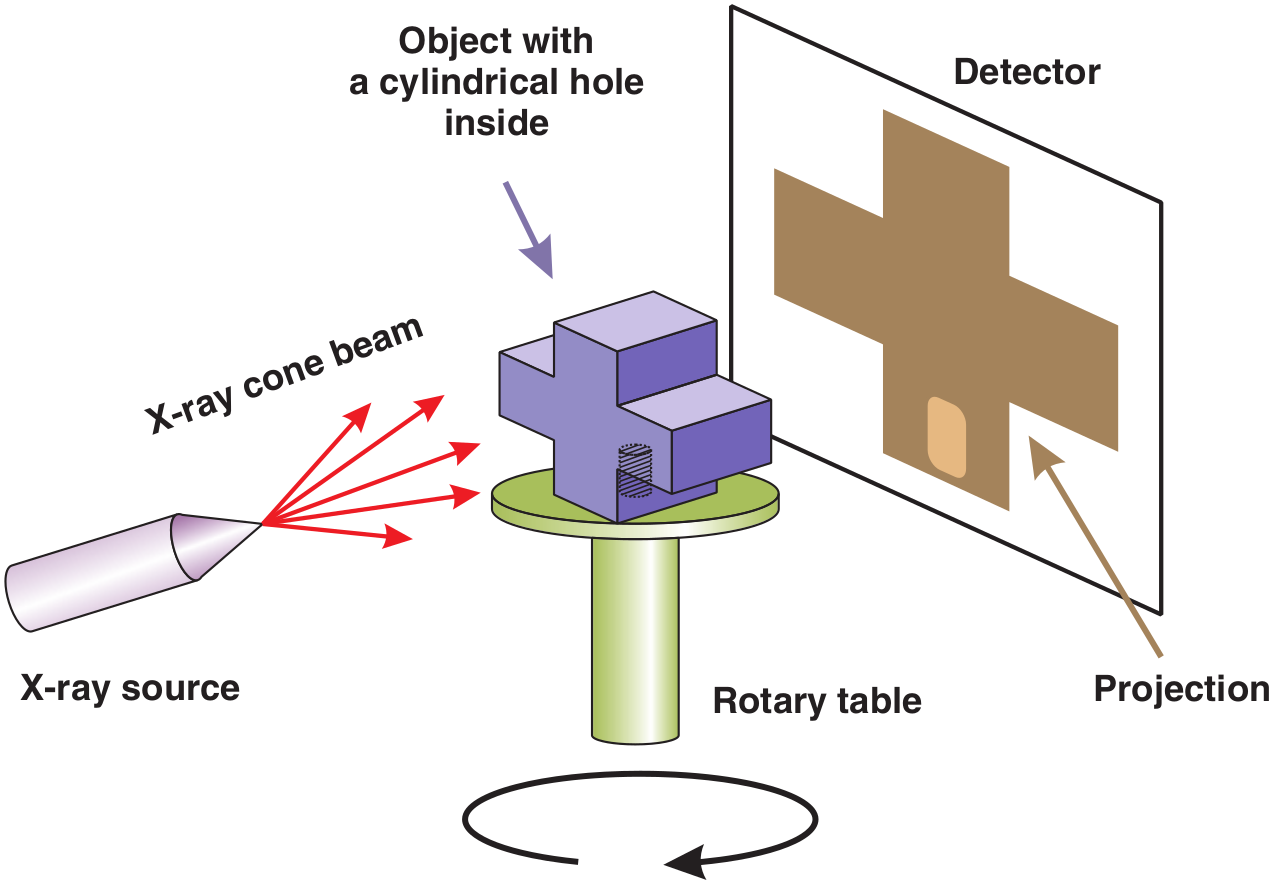
\includegraphics[width=0.75\textwidth]{../figures/literatureReview/literature_xct.png}
  \caption{The setup of XCT used in metrology. Reprinted from \cite{warnett2016towards} under the CC BY 3.0 license.}
  \label{fig:literature_xct}
\end{figure}

The acquisition process consists of the production of x-rays, x-rays attenuating the object, the detection of x-rays and the reconstruction process.

X-rays \citep{rontgen1896on} are produced in an x-ray tube, a diagram shown in Figure \ref{fig:literature_tube}. It consists of a vacuum tube containing a cathode and an anode. Electrons are fired from the cathode to the anode due to an electric potential. The cathode is usually tungsten and the anode contains a small amount of tungsten, molybdenum or copper \citep{sun2012overview}.

\begin{figure}
  \centering
  
\includegraphics[width=0.8\textwidth]{../figures/literatureReview/literature_tube.png}
  \caption{An x-ray tube. Reprinted from \cite{michael2001x}. \textcopyright\ IOP Publishing. Reproduced with permission. All rights reserved.}
  \label{fig:literature_tube}
\end{figure}

The electrons can interact with the anode in many ways. The electrons can be deflected or decelerated due to the electric field from the nucleus of the target anode material. The energy lost by the electrons is emitted as bremsstrahlung radiation. The energy of the radiation depends on the potential difference in the x-ray tube, as this determines the energy of the fired electrons, and also the proton number of the anode target because this affects the electric field produced by the nucleus in the anode target \citep{sun2012overview}. Another interaction is when the electrons may collide with the nucleus in the anode target, exciting an inner shell electron and ionizing it. This produces a vacancy in the electron shell and emits a photon when the excited electron drops down back to the ground state. This is known as characteristic radiation and the energy emitted is discrete and depends on the material in the anode target \citep{sun2012overview}.

The efficiency of an x-ray tube is poor. Over 99\% of the energy from electrons is converted to heat, the rest to x-rays \citep{kruth2011computed}.

Photons, making up the radiation, are emitted from the x-ray tube which can be modelled as a Poisson process \citep{whiting2006properties, cierniak2011x}. The rate of x-ray emission depends on the current, that is the rate of charge between the cathode and anode. Sources of energy of each photon come from bremsstrahlung radiation and characteristic radiation, making the distribution of x-ray photons energy a mix of continuous and discrete energies \citep{sun2012overview}. An example is shown in Figure \ref{fig:literature_spectrum}.

\begin{figure}
  \centering
  
\includegraphics[width=0.65\textwidth]{../figures/literatureReview/literature_spectrum.png}
  \caption{An example of the distribution of energies a photon can have emitted from an x-ray tube. Bremsstrahlung and characteristic radiation contribute to the continuous and discrete components of the distribution. Reprinted from \cite{michael2001x}. \textcopyright\ IOP Publishing. Reproduced with permission. All rights reserved.}
  \label{fig:literature_spectrum}
\end{figure}

The scanned object is exposed to x-ray photons which undergo attenuation when interacting with the object in several ways \citep{cantatore2011introduction}. The object can absorb the photons via the photoelectric effect. In the photoelectric effect, a photon transfer all of its energy to a bounded electron and ejects it from the atom in the object \citep{millikan1916direct}. Photons can be scattered by the object by colliding inelastically with and transfers its energy to an electron. This process is known as Compton scattering \citep{compton1923quantum}. The photoelectric effect and Compton scattering cause several photons to be undetectable. If some of the photons avoid these processes, they are detected and their energy is left unaffected.

Beer's law simplifies these quantum mechanistic process. Suppose the x-ray beam with a rate of emission $I_0$ is mono-energetic and travels in a straight line in the $x$-axis. Let $\mu(x)$ be the attenuation coefficient of the object and the x-ray beam has a rate of emission $I$ after attenuation. A differential equation can be set up to model the decay of photons as it attenuates through the object such that
\begin{equation}
\dfrac{\diff I}{\diff x} = -I\mu(x)
\end{equation}
which can be solved
\begin{equation}
I = I_0\exp\left[\int_{x \in \text{path of photon}}-\mu(x)\diff x\right] \ .
\label{eq:beerLaw}
\end{equation}
However, the photoelectric effect and Compton scattering, thus the attenuation coefficient as well, depends on the energy of the photons \citep{elbakri2002statistical}. Therefore $\mu(x,E)$ should be made dependent on the energy of the photons \citep{cantatore2011introduction} and can cause some inaccuracies in Beer's law. In general low energy photons are more likely to be absorbed and scattered than high energy photons, which increases the average energy of the detected photons \citep{sun2012overview}. This is called beam hardening.

After attenuation, the x-ray photons are detected by the x-ray detector. The detectors used in XCT are typically flatbed scanners made up of a scintillator material \citep{curran1953luminescence, greskovich1997ceramic} and photodiodes. The x-ray photons interact with the scintillator material and produce visible light pluses \citep{rossner1993conversion}. These pulses are detected by photodiodes and converted into an electrical signal \citep{nikl2006scintillation, ren2018tutorial}. The electrical signal can be a quantum counter, counting the number of photons detected, or an energy integrating detector, adding up all of the energies of each detected photon \citep{nikl2006scintillation, whiting2006properties, kruth2011computed, ren2018tutorial}. The electrical signals are subject to sampling and quantisation to store these signals as an image \citep{cierniak2011x}. This image is known as a projection.

Not all of the visible light pulses are detected by the photodiodes, thus not all the x-ray photons are detected. The ratio between the number of x-ray photons detected by the detector and the number of x-ray photons arriving at the detector is called the quantum efficiency \citep{cierniak2011x, ren2018tutorial}. This makes the detection a two-stage process, converting the x-ray photons into visible light which are then detected \citep{cierniak2011x}. There exist equipment which detects x-ray directly such as a xenon gas ionisation detector \citep{fuchs2000direct} but this is unrivalled by solid-state CT systems, such as scintillator-photodiodes detectors, which have a high quantum efficiency of about 98\% to 99.5\% \citep{hsieh2000investigation}.

Once projections of the object have been acquired at multiple angles, the reconstruction process can start. The objective of reconstruction is to estimate the attenuation coefficient of the object at each point in space $\mu(x,y,z)$ using the x-ray projections. This is done using the fact that the projections are based on the line integral of the attenuation coefficient along the path of photons. This problem was formed by \cite{radon1986on} as the `determination of functions from their integral values along certain manifolds'.

A number of reconstruction algorithms in XCT have been developed \citep{smith1990cone} such as the filtered back-projection \citep{brooks1976principles} and the FDK algorithm \citep{feldkamp1984practical}. Once the reconstruction has been done, the shape or surface can be extracted by the use of thresholding \citep{kruth2011computed}. There are many software packages available for the reconstruction stage of XCT \citep{reinhart2008industrial, sun2012overview}.

\subsection{Metrology in Practice}

XCT can be used to measuring lengths and distances, making it useful for measuring the dimensions of AM objects internally and externally. \emph{Nikon} offer products and services for XCT including features such as direct comparison to the CAD model \citep{nikon2015microfocus, nikon2018mct225} and automated production line inspection \citep{nikon2015inline, nikon2018automated}.

As with a lot of measurement apparatus, calibration is required. In XCT, the scale of each voxel in the reconstruction can be obtained by using XCT on an object with pre-determined lengths, these are known as reference standards \citep{bartscher2007enhancement} but can have similar names. Reference standards can vary in geometry such as a sphere on a cylinder \citep{lifton2013application}, two spheres on a cylinder \citep{sun2016reference}, a cube with cut-outs \citep{kiekens2011test}, a hollow cylinder, a step-cylinder and a ball-bar \citep{bartscher2007enhancement}; the latter three are shown in Figure \ref{fig:literature_referenceStandards}.

\begin{figure}
  \centering
  \centerline{
    \begin{subfigure}[b]{0.49\textwidth}
      
\includegraphics[width=\textwidth]{../figures/literatureReview/literature_test1.png}
      \caption{Hollow cylinder}
    \end{subfigure}
    \begin{subfigure}[b]{0.49\textwidth}
      
\includegraphics[width=\textwidth]{../figures/literatureReview/literature_test2.png}
      \caption{Step-cylinder}
    \end{subfigure}
  }
  \begin{subfigure}[b]{0.6\textwidth}
    
\includegraphics[width=\textwidth]{../figures/literatureReview/literature_test3.png}
    \caption{Ball-bar}
  \end{subfigure}
  \caption{Various reference standards: a) aluminium hollow cylinder, outer diameters \SI{30}{\milli\metre} and \SI{20}{\milli\metre}, b) aluminium step-cylinder with diameter \SI{300}{\milli\metre}, c) ceramic balls of diameter \SI{30}{\milli\metre} on a carbon fibre rod, the balls are separated by \SI{100}{\milli\metre}. Reprinted from \cite{bartscher2007enhancement}\textsuperscript{\textcopyright} with permission from Elsevier.}
  \label{fig:literature_referenceStandards}
\end{figure}

There are many variables in XCT and a lot of them have to be controlled, for example, XCT should be done in room temperature to avoid any thermal variation \citep{bryan1990international}, however, this can be hard to do when the x-ray tube is a heat source \citep{kruth2011computed}.

The potential difference and current of the x-ray tube can be adjusted to control the contrast and brightness of the x-ray projection. The exposure time is also a factor. These settings should be set high enough to avoid beam extinction but low enough that there is a contrast where less material is present \citep{kruth2011computed}.

The magnification can be modified by altering the distances between the x-ray tube, the object and the x-ray detector. Increasing the magnification increases the image resolution but can cause blurry images, this is the result of using an x-ray source with a finite spot size as shown in Figure \ref{fig:literature_magnification} \citep{kruth2011computed}. Larger spot sizes cause more blurry results, this is known as the penumbra effect \citep{kueh2016modelling}. However, spot sizes too small can produce concentrated heat \citep{welkenhuyzen2009industrial} and can damage the x-ray tube.

\begin{figure}
  \centering
  
\includegraphics[width=0.7\textwidth]{../figures/literatureReview/literature_magnification.png}
  \caption{The magnification can be adjusted by adjusting the distances between the x-ray source, the object and the x-ray detector. Because of a finite x-ray spot size, blurry effects are produced using a magnification too large. Reprinted from \cite{kruth2011computed}\textsuperscript{\textcopyright} with permission from Elsevier.}
  \label{fig:literature_magnification}
\end{figure}

There is also the question on how to orient the object on the turntable \citep{corcoran2016observations} as well as how many angles to use \citep{kruth2011computed}. More angles produce a more accurate reconstruction but require more acquisition time. Figure \ref{fig:literature_angles} shows an example of a reconstruction using various numbers of angles.

\begin{figure}
  \centering
  
\includegraphics[width=0.7\textwidth]{../figures/literatureReview/literature_angles.png}
  \caption{A reconstruction when scanning three aligned balls using a different number angular projections. Reprinted from \cite{kruth2011computed}\textsuperscript{\textcopyright} with permission from Elsevier.}
  \label{fig:literature_angles}
\end{figure}

All of the parameters of XCT discussed can be determined before the XCT process by use of simulations \citep{reisinger2011simulation, reiter2011simulation}, however, there may be inconsistencies. For example, even though the target material of the anode and power is specified, the energy spectrum can still vary \citep{stumbo2004direct}.

Problems can occur in the detector, for example, pixels in the acquired projection can be defective or dead \citep{brettschneider2014spatial}, the panel structure of the detector can be observed \citep{yang2009evaluation} and the cone-beam appears as a spot. The x-ray spot could be fitted by using a mixture of a Gaussian spot and a uniform spot \citep{kueh2016modelling}. Another problem is that there exist spatially correlated noise within a projection which can be detected experimentally \citep{sun2016characterisation} as well as a correlation between acquisitions, known as image lag \citep{yang2009evaluation}. Precautions can be taken to reduce the impact from image lag such as waiting for 20 minutes between acquisitions \citep{yang2010noise}.

Errors due to beam hardening can occur. Low energy photons are more likely to be absorbed or scattered, which causes a few millimetres of the surface of the object to absorb or scatter more photons than the interior. This can cause artefacts \citep{sun2016applications} such as flat surfaces to be barrelled and edges rounded off \citep{kruth2011computed}. Beam hardening can be tackled by eliminating the low energy photons by placing a filter, a thin metal plate, in front of the x-ray tube \citep{welkenhuyzen2009industrial}, for example, copper. Figure \ref{fig:literature_hardening} shows an example of reconstruction with and without a filter. Without the filter, the outer perimeter appears less dense than it should be.  A filter reduces the rate of photon emission but this can be compensated by increasing the exposure time \citep{kruth2011computed}. Early reconstruction algorithms ignored beam hardening but modern methods can take beam hardening into account \citep{elbakri2001statistical, sun2016applications}.

\begin{figure}
  \centering
    \begin{subfigure}[b]{0.4\textwidth}
      
\includegraphics[width=\textwidth]{../figures/literatureReview/literature_hardening_noFilter.png}
      \caption{No filter}
    \end{subfigure}
    \begin{subfigure}[b]{0.4\textwidth}
      
\includegraphics[width=\textwidth]{../figures/literatureReview/literature_hardening_filter.png}
      \caption{Al/Cu filter}
    \end{subfigure}
  \caption{A reconstruction of a hollow cylinder, outer diameter \SI{6.0}{\milli\metre} and inner diameter \SI{0.6}{\milli\metre}. In a), no filter was used. In b) a filter was placed in front of the x-ray tube. Reprinted from \citep{kruth2011computed}\textsuperscript{\textcopyright} with permission from Elsevier}
  \label{fig:literature_hardening}
\end{figure}

The most common reconstruction method is the FDK \citep{feldkamp1984practical} algorithm because it caters for cone beams. However, it assumes a circular trajectory from the source which can cause artefacts if the trajectory is not circular \citep{sun2016applications}.

\subsection{Latest Research}

The most common use of XCT in AM is the investigation of pores in the manufactured object \citep{thompson2016x}. Pores can be classified as defects if the pores are larger than some volume threshold. This threshold controls the probability of the detection of defects \citep{gandossi2010probability, amrhein2014characterization}.

The porosity is defined by dividing the volume of all of the pores by the volume of solid material \citep{taud2005porosity}. This can be used to quantified the material's strength and can be measured accurately using Archimedes' method \citep{spierings2011comparison}. Studies have been done to link porosity to stress concentration \citep{leuders2015fatigue, siddique2015computed, carlton2016damage} and it was found the location of the pores is a good predictor of fatigue strength \citep{leuders2015fatigue}. XCT can be used to measure porosity and has an advantage over Archimedes' method because the location of the pores can be visualised in XCT. An example of visualising pores is shown in Figure \ref{fig:literature_pores3D} and the pores can be compared to the CAD model \citep{lee2015compliance, villarraga2015assessing, kim2016inspection}. In addition to pores, any surface deviation can be measured by aligning the reconstruction with the CAD model and measuring any discrepancies \citep{lee2015compliance, villarraga2015assessing, kim2016inspection}, an example is shown in Figure \ref{fig:literature_warnett}.

\begin{figure}
  \centering
      \begin{subfigure}[b]{0.49\textwidth}
      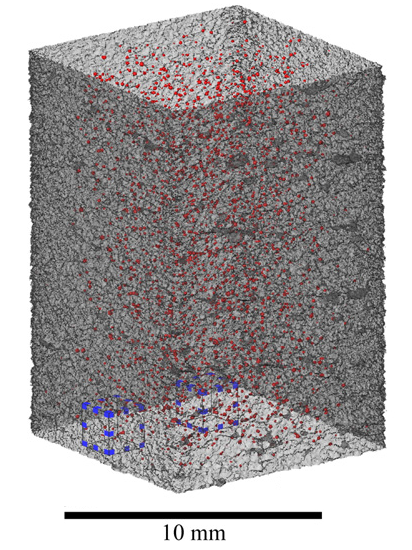
\includegraphics[width=\textwidth]{../figures/literatureReview/literature_pores3D1.png}
      \caption{Reconstruction}
    \end{subfigure}
    \begin{subfigure}[b]{0.49\textwidth}
      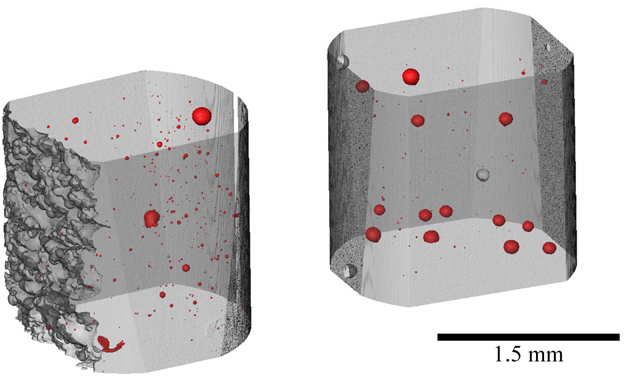
\includegraphics[width=\textwidth]{../figures/literatureReview/literature_pores3D2.png}
      \caption{Sample from the reconstruction}
    \end{subfigure}
    \caption{The reconstruction can show pores in the manufactured object. b) shows the reconstructed samples from the blue cubes in a). Reprinted from \cite{tammas2015xct} under the CC BY 4.0 license.}
    \label{fig:literature_pores3D}
\end{figure}

\begin{figure}
  \centering
      \begin{subfigure}[b]{0.49\textwidth}
      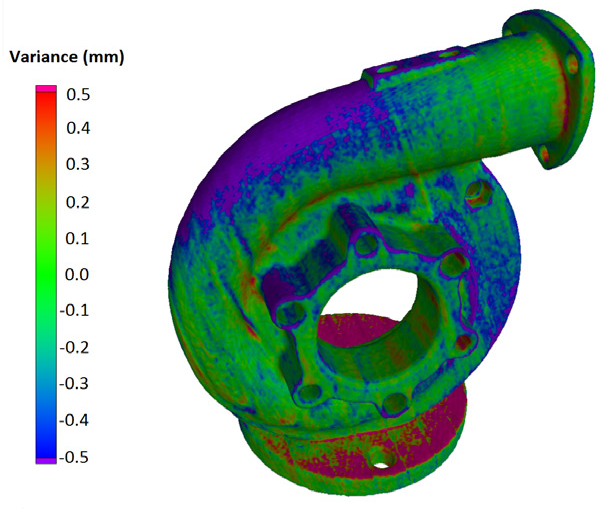
\includegraphics[width=\textwidth]{../figures/literatureReview/literature_warnett1.png}
      \caption{External}
    \end{subfigure}
    \begin{subfigure}[b]{0.49\textwidth}
      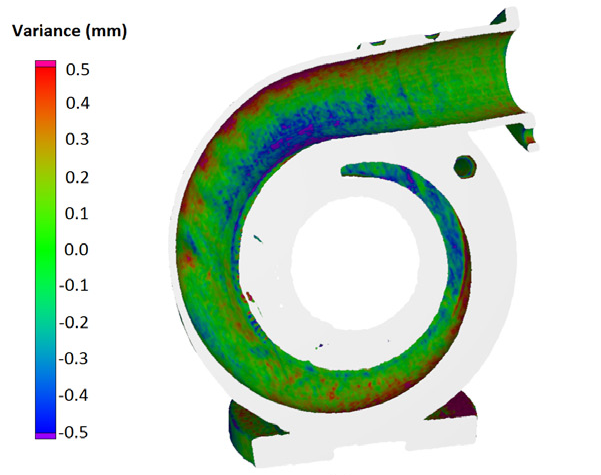
\includegraphics[width=\textwidth]{../figures/literatureReview/literature_warnett2.png}
      \caption{Internal}
    \end{subfigure}
    \caption{The reconstruction was aligned and compared to the CAD model. The surface heat map shows the surface deviation (or `variance' in the literature) externally (a) and internally (b). Reprinted from \cite{warnett2016towards} under the CC BY 3.0 license.}
    \label{fig:literature_warnett}
\end{figure}

One of the disadvantages of XCT is that it is a slow process. XCT is not an instantaneous process so progress bars are usually featured in XCT marketing such as \cite{nikon2015inline}'s inline quality control. The reconstruction can take between 5 minutes to several hours \citep{warnett2016towards}. More angular projections would take more time but will improve the accuracy of the reconstruction \citep{kruth2011computed}. \cite{warnett2016towards} improved the speed of XCT by sacrificing the accuracy of the reconstruction. This was done by placing the object on a conveyor belt surrounded by multiple x-ray source and detector pairs as shown in Figure \ref{fig:literature_conveyor}. Fewer angular projections were taken but they can be obtained in one go, speeding up the process.

\begin{figure}
  \centering
  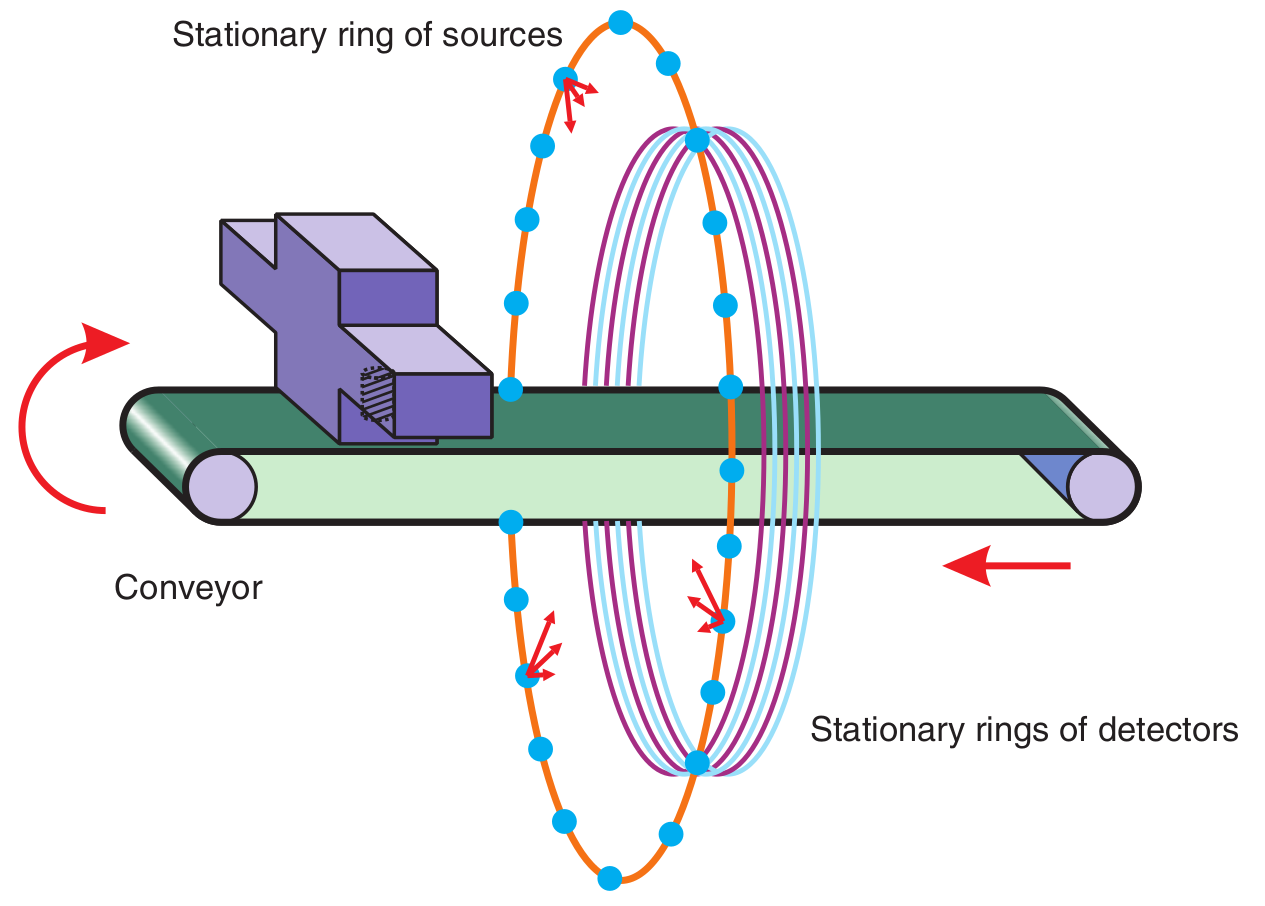
\includegraphics[width=0.7\textwidth]{../figures/literatureReview/literature_conveyor.png}
  \caption{XCT can be done on a conveyor belt surrounded by x-ray source and detector pairs. Reprinted from \cite{warnett2016towards} under the CC BY 3.0 license.}
  \label{fig:literature_conveyor}
\end{figure}

Instead of reconstructing the object, the analysis can be done on the projections itself, or in projection space, by comparing it to a simulated projection produced by a software called \emph{aRTist} \citep{bellon2007artist, jaenisch2008artist, bellon2012radiographic}. It can simulate projections of the object given the specifications of the CT apparatus, such as the x-ray source and the x-ray detector, and the CAD of the object \citep{bellon2011simulation, deresch2012simulating}.

An algorithm was developed to adjust the parameters of the simulation as well as aligning it so that it fits with the x-ray acquisition \citep{brierley2018optimized}. However, it is very complicated as it is optimising over a very large dimensional space \citep{brierley2018optimized}. It was demonstrated that detection of defects is possible in projection space by comparing two simulated projections with each other, one with defects and the other without \citep{brierley2018optimized}. Another method is to use machine learning methods to classify defects from a projection \citep{rale2009comparison}.

It is however inevitable that accuracy is lost from the transition from reconstruction space to projection space, for example, in the diagnostic of pneumonia, a CT scan has superior performance compared to a chest radiograph \citep{hayden2009chest}.

\chapter{Data Collection}
\label{chapter2}
The objective is to investigate if voids can be detected using a single projection. The quality control procedure can be sped up if defect detection can be done in projection space rather than reconstruction space. An experiment was conducted where a test sample was additively manufactured with purposely designed voids. This was done by comparing a projection of the test sample with the simulation of that projection as if the voids were not there. The simulated projections were produced by using software called \emph{aRTist} \citep{bellon2007artist, jaenisch2008artist, bellon2012radiographic}. Any disagreement in the comparison can suggest evidence of a defect.

This chapter describes the apparatus used to manufacture the test sample and obtaining the projections. There is also a discussion, at the end of the chapter, on shading correction which was used to remove panel and x-ray spot effects from the projections.

Many figures presented here were given by engineers concerning the experiment or by the manufacturer. Figures with no error bars were rounded to an appropriate number of significant figures.

\section{Apparatus}

The test object is a cuboid (\SI{40.0}{\milli\metre} $\times$ \SI{40.0}{\milli\metre} $\times$ \SI{60.0}{\milli\metre}) with voids. The voids were of diameters \SI{2.4}{\milli\metre}, \SI{1.2}{\milli\metre}, \SI{0.6}{\milli\metre} and \SI{0.3}{\milli\metre}. 6 voids for each diameter were designed in the CAD. Voids with diameters \SI{2.4}{\milli\metre} and \SI{0.6}{\milli\metre} were regularly arranged, the other ones were arranged irregularly. The CAD model of the test sample is shown in Figure \ref{fig:inference_testObject}.

\begin{figure}
  \centering
  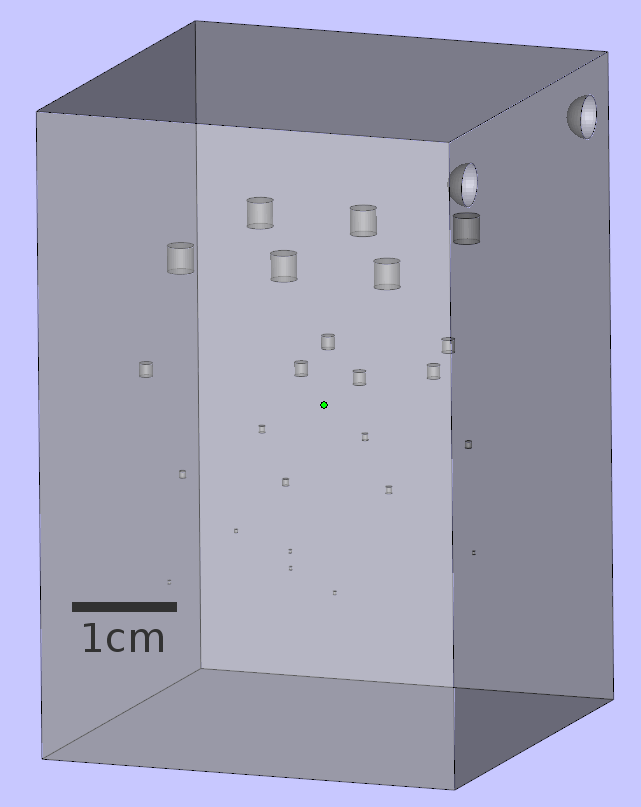
\includegraphics[width=0.4\textwidth]{../figures/inference/TestObject.png}
  \caption{CAD model of the test sample; the scale shown is approximate.}
  \label{fig:inference_testObject}
\end{figure}

The \emph{Fortus 400mc (Stratasys, US)} was used to manufacture the test object made of plastic (acrylonitrile butadiene styrene or ABS). The precision of the manufacturing was in the order of $\pm\SI{0.1}{\milli\metre}$ \citep{hanseen2013fortus}. Another test object was manufactured made from titanium (Ti-6Al-4V)

X-ray projections were obtained using the \emph{Nikon XT H LC 225/320} x-ray CT scanner (\emph{Nikon Metrology, UK}) together with a \emph{Perkin Elmer XRD 1621 (Perkin Elmer, US)} detector. The target material in the x-ray tube was tungsten. The detector was made up of 2 rows and 16 columns of panels and together has dimensions of $\SI{409.6}{\milli\metre}\times\SI{409.6}{\milli\metre}$ which produced a 16-bit projection of $\SI{2048}{\pixel}\times\SI{2048}{\pixel}$ in size \citep{perkinelmer2006xrd}. Therefore, the scale of each pixel is $\SI{200.0}{\micro\metre\per\pixel}$. The projections were cropped to $\SI{2000}{\pixel}\times\SI{2000}{\pixel}$ to remove boundary effects. The gain and offset were adjusted by the engineers to produce a projection with good contrast and negligible penumbra effect. Each pixel has a grey value in units of analogue to digital units (\SI{}{\adu}).

Greyscale projections were taken in addition to the projection of the test object. These are projections with nothing between the source and the detector, obtained with the x-ray tube at different powers. The power was varied by fixing the potential difference and varying the current. The greyscale projections were used for calibration such as shading correction. The greyscale projection with the x-ray turned off is called the black image. The greyscale projection with the x-ray set up the same when obtaining the test sample projection is called the white image.

Replicate test sample projections and greyscale projections were obtained by repeating the acquisition. These replicated projections were used to study the noise observed in the projections.

Filters were used, such as a \SI{0.35}{\milli\metre} copper filter and a \SI{2.0}{\milli\metre} tin filter, to tackle beam hardening.

\emph{aRTist} was used to simulate the test object projection and all greyscale projections except for the black image. The black image was simulated by producing a uniform image with a grey value the mean over the obtained black image. The engineers used numerical methods to align the simulated projection with the obtained projection.

\section{Datasets}

Three datasets were collected and named \texttt{AbsNoFilter}, \texttt{AbsFilter} and \texttt{TiFilter}. They contain replicate projections of the test sample at two different angles, named $\ang{30}$ and $\ang{120}$, as well as replicate greyscale projections. Projections of the ABS test sample were taken in \texttt{AbsNoFilter} and \texttt{AbsFilter}. The titanium test sample was scanned in \texttt{TiFilter}. To investigate the effects of beam hardening, no x-ray filter was used in \texttt{AbsNoFilter}, a filter was used in \texttt{AbsFilter} and \texttt{TiFilter}.

The properties of each dataset are shown in Table \ref{table:data_dataset}. These include the properties of the x-ray tube, the XCT apparatus and what powers were used in the greyscale projections. A sample of the obtained, simulated and greyscale projections for the datasets \texttt{AbsNoFilter}, \texttt{AbsFilter} and \texttt{TiFilter} are shown in Figures \ref{fig:data_AbsNoFilter}, \ref{fig:data_AbsFilter} and \ref{fig:data_TiFilter} respectively.

\begin{sidewaystable}
\centering
\begin{tabular}{l|lll}
                                                       & \multicolumn{3}{c}{Dataset name}                                                \\
                                                       & \texttt{AbsNoFilter} & \texttt{AbsFilter}             & \texttt{TiFilter}        \\ \hline
potential difference (\SI{}{\kilo\volt})               & 80                   & 80                             & 190                      \\
power (\SI{}{\watt})                                   & 36                   & 20                             & 20                       \\
filter                                                 & no filter            & \SI{0.35}{\milli\metre} copper & \SI{2.0}{\milli\metre} tin \\
time exposure (\SI{}{\milli\second})                   & 708                  & 500                            & 1415                     \\
distance from source to object (\SI{}{\milli\metre})   & 217                  & 168                            & 86                       \\
distance from source to detector (\SI{}{\milli\metre}) & 1178                 & 876                            & 875                      \\
number of replications for each angle                  & 100                  & 20                             & 20                       \\ \hline
powers used for greyscale projections (\SI{}{\watt})   & 0.0                  & 0.0                            & 0.0                      \\
\multicolumn{1}{c|}{\vdots}                            & 10                   & 5.0                            & 10                       \\
\multicolumn{1}{c|}{\vdots}                            & 18                   & 10                             & 20                       \\
\multicolumn{1}{c|}{\vdots}                            & 28                   & 15                             &                          \\
\multicolumn{1}{c|}{\vdots}                            & 36                   & 20                             &                          \\
number of replications for each power                  & 20                   & 20                             & 20                    
\end{tabular}
\caption{Properties of the three datasets obtained for the experiment.}
\label{table:data_dataset}
\end{sidewaystable}

\begin{figure}[p]
  \centering
  \centerline{
    \begin{subfigure}[b]{\subSize}
      \includegraphics[width=\textwidth]{../figures/data/AbsNoFilterDeg30.eps}
      \caption{Obtained projection at \SI{36}{\watt}}
    \end{subfigure}
    \begin{subfigure}[b]{\subSize}
      \includegraphics[width=\textwidth]{../figures/data/AbsNoFilterDeg30_sim.eps}
      \caption{Simulated projection at \SI{36}{\watt}}
    \end{subfigure}
  }
  \centerline{
    \begin{subfigure}[b]{\subSize}
      \includegraphics[width=\textwidth]{../figures/data/AbsNoFilter_calibration1.eps}
      \caption{Greyscale projection at \SI{0}{\watt}}
    \end{subfigure}
    \begin{subfigure}[b]{\subSize}
      \includegraphics[width=\textwidth]{../figures/data/AbsNoFilter_calibration5.eps}
      \caption{Greyscale projection at \SI{36}{\watt}}
    \end{subfigure}
  }
  \caption{\texttt{AbsNoFilter} projections at \ang{30}; note the colour scale may vary.}
  \label{fig:data_AbsNoFilter}
\end{figure}

\begin{figure}[p]
  \centering
  \centerline{
    \begin{subfigure}[b]{\subSize}
      \includegraphics[width=\textwidth]{../figures/data/AbsFilterDeg30.eps}
      \caption{Obtained projection at \SI{20}{\watt}}
    \end{subfigure}
    \begin{subfigure}[b]{\subSize}
      \includegraphics[width=\textwidth]{../figures/data/AbsFilterDeg30_sim.eps}
      \caption{Simulated projection at \SI{20}{\watt}}
    \end{subfigure}
  }
  \centerline{
    \begin{subfigure}[b]{\subSize}
      \includegraphics[width=\textwidth]{../figures/data/AbsFilter_calibration1.eps}
      \caption{Greyscale projection at \SI{0}{\watt}}
    \end{subfigure}
    \begin{subfigure}[b]{\subSize}
      \includegraphics[width=\textwidth]{../figures/data/AbsFilter_calibration5.eps}
      \caption{Greyscale projection at \SI{20}{\watt}}
    \end{subfigure}
  }
  \caption{\texttt{AbsFilter} projections at \ang{30}; note the colour scale may vary.}
  \label{fig:data_AbsFilter}
\end{figure}

\begin{figure}[p]
  \centering
  \centerline{
    \begin{subfigure}[b]{\subSize}
      \includegraphics[width=\textwidth]{../figures/data/TiFilterDeg30.eps}
      \caption{Obtained projection at \SI{20}{\watt}}
    \end{subfigure}
    \begin{subfigure}[b]{\subSize}
      \includegraphics[width=\textwidth]{../figures/data/TiFilterDeg30_sim.eps}
      \caption{Simulated projection at \SI{20}{\watt}}
    \end{subfigure}
  }
  \centerline{
    \begin{subfigure}[b]{\subSize}
      \includegraphics[width=\textwidth]{../figures/data/TiFilter_calibration1.eps}
      \caption{Greyscale projection at \SI{0}{\watt}}
    \end{subfigure}
    \begin{subfigure}[b]{\subSize}
      \includegraphics[width=\textwidth]{../figures/data/TiFilter_calibration3.eps}
      \caption{Greyscale projection at \SI{20}{\watt}}
    \end{subfigure}
  }
  \caption{\texttt{TiFilter} projections at \ang{30}; note the colour scale may vary.}
  \label{fig:data_TiFilter}
\end{figure}

The projections show the test sample, but, with panel and spot effects. The structure of the 32 panels are predominate in the black image, in particular, this was observed by \cite{yang2009evaluation} as well. This is concerning because systematic errors could be introduced as a result of the panel effects in the black image. This should not happen because, in a black image, the detector is exposed only to background radiation. The x-ray spot can be observed, in particular, in the white image, and this is the result of using a cone beam.

\afterpage{\clearpage}

\section{Shading Correction}

Shading correction, also known as flat field correction, aims to eliminate any spatial variation in sensitivity, observed in the projections, as a result from panel effects, spot effects and other artefacts. Shading correction is done by using the greyscale projections and examining how the grey values respond to different powers for different pixels. For example, the black and white image can be used to correct the projections using
\begin{equation}
U_{x,y} = \dfrac{N_{x,y}-\text{black}_{x,y}}{\text{white}_{x,y}-\text{black}_{x,y}}\times B+A
\label{eq:data_shadingCorrectionOld}
\end{equation}
where $N_{x,y}$ is the obtained projection, $U_{x,y}$ is the shading corrected projection and $A$ and $B$ are some user defined constants \citep{young2000shading, munzenmayer2003enhancing}. This can be extended to include more greyscale projections by modelling the grey value to respond linearly to the power of the x-ray source \citep{seibert1998flat}. More generally, shading correction can be expressed as
\begin{equation}
U_{x,y} = \beta_{x,y} N_{x,y} + \alpha_{x,y}
\end{equation}
where $\alpha_{x,y}$ and $\beta_{x,y}$ are some spatially varying functions \citep{munzenmayer2003enhancing}. This model has limitations because $\alpha_{x,y}$ and $\beta_{x,y}$ may depend on the energy of each photon, thus beam hardening could cause inaccuracies in shading correction \citep{davidson2003limitations}. Other methods include minimising the entropy of the projection while constraining $\alpha_{x,y}$ and $\beta_{x,y}$ to be some parametric function \citep{likar2000retrospective} and using a low pass filter to remove low spatial frequencies from the projections \citep{young2000shading, munzenmayer2003enhancing}.

In this section, the shading correction in \cite{seibert1998flat} is presented in a form without any user-defined constants. The shading correction was experimented to investigate its performance when shading correcting greyscale projections.

\subsection{Proposed Shading Correction}

Let $S_{x,y}(P)$ be the greyscale projection when exposed to x-rays produced by an x-ray tube with power $P$ for some fixed time exposure $\tau$. $S_{x,y}(P)$ may be averaged over replications. Let $x=1,2,3,\dotsc, W$ and $y=1,2,3,\dotsc,H$. Let $N_{x,y}$ be the obtained projection of the test sample when exposed to x-rays produced by an x-ray tube with power $P_\text{proj}$ for some fixed time exposure $\tau$. The black and white image can be expressed as $\text{black}_{x,y}=S_{x,y}(0)$ and $\text{white}_{x,y}=S_{x,y}(P_\text{proj})$ respectively. For both the greyscale projections and the projection of the test sample, the power was varied by fixing the potential difference and varying the current of the x-ray tube.

The shading free image is not known, but it is expected that the shading corrected greyscale projection should be flat with some noise. In other words, all pixels in a shading corrected greyscale projection should have grey values with the same expectation $\mu_{S}(P)$ and same variance $\sigma_{S}^2(P)$. Suppose $\mu_{S}(P)$ was estimated using the within projection mean
\begin{equation}
\overline{S}(P) = \dfrac{1}{\text{WH}}
\sum_{x=1}^W\sum_{y=1}^H S_{x,y}(P) \ .
\end{equation}
Consider a pixel at $(x,y)$, shading correction was done by fitting a linear regression on
\begin{equation}
\overline{S}(P) = \beta_{x,y} S_{x,y}(P) + \alpha_{x,y} \quad(+\varepsilon)
\end{equation}
for $P\in \mathbb{P}$ where $\mathbb{P} = \left\{0,P_1,P_2,\cdots, P_\text{proj}\right\}$ are the powers used for the greyscale projections. $\varepsilon$ is a random variable and an error term, it is included for formality purposes. Let $b_{x,y}$ and $a_{x,y}$ be the estimated parameters of $\beta_{x,y}$ and $\alpha_{x,y}$ from the linear regression respectively. Given a projection $N_{x,y}$, the shading corrected projection $U_{x,y}$ is
\begin{equation}
U_{x,y} = b_{x,y} N_{x,y} + a_{x,y} \ .
\end{equation}
In full, the equations for $b_{x,y}$ and $a_{x,y}$ are given as
\begin{equation}
b_{x,y} = \dfrac{
  \sum_{P\in\mathbb{P}}(S_{x,y}(P) - \overline{S}_{x,y})(\overline{S}(P) - \overline{S})
}{
  \sum_{P\in\mathbb{P}}(S_{x,y}(P) - \overline{S}_{x,y})^2
}
\end{equation}
and
\begin{equation}
a_{x,y} = \overline{S} - b_{x,y}\overline{S}_{x,y}
\end{equation}
where $\overline{S}_{x,y}$ is the between projection mean
\begin{equation}
\overline{S}_{x,y} = \dfrac{1}{|\mathbb{P}|}\sum_{P\in\mathbb{P}}S_{x,y}(P)
\end{equation}
and $\overline{S}$ is the global mean
\begin{equation}
\overline{S} = \dfrac{1}{|\mathbb{P}|}\sum_{P\in\mathbb{P}}\overline{S}(P) \ .
\end{equation}
This type of shading correction shall be referred to as linear shading correction. Expressing shading correction in this way has the advantage that there are no user defined constants.

An example of the linear regression is shown in Figure \ref{fig:data_shadingCorrectionExample_gainMap} where 3 random pixels were chosen for illustration. By plotting the within projection mean versus the grey value for a particular pixel, a linear relationship can be observed. The gradient varied for different pixels which correspond to different sensitivities. The resulting shading correction for the \texttt{AbsNoFilter} projection is shown in Figure \ref{fig:data_shadingCorrectionExample_image}. It can be observed that the shading correction removed the panel and spot effects from the background and test sample.

\begin{figure}
  \centering
  \centerline{
    \begin{subfigure}[b]{\subSize}
      \includegraphics[width=\textwidth]{../figures/data/shadingCorrectionExample_interpolation.eps}
      \caption{Linear regression}
    \end{subfigure}
    \begin{subfigure}[b]{\subSize}
      \includegraphics[width=\textwidth]{../figures/data/shadingCorrectionExample_gradient_linear.eps}
      \caption{$b_{x,y}$}
    \end{subfigure}
  }
  \caption{For each pixel, a linear regression was fitted on the within projection mean versus the grey value for each greyscale projection. The \texttt{AbsNoFilter} dataset was used. 3 random pixels were used to illustrate this in a). b) shows the fitted gradient for all pixels.}
  \label{fig:data_shadingCorrectionExample_gainMap}
\end{figure}

\begin{figure}
  \centering
  \centerline{
    \begin{subfigure}[b]{\subSize}
      \includegraphics[width=\textwidth]{../figures/data/shadingCorrectionExample_image_null.eps}
      \caption{No shading correction}
    \end{subfigure}
    \begin{subfigure}[b]{\subSize}
      \includegraphics[width=\textwidth]{../figures/data/shadingCorrectionExample_image_linear.eps}
      \caption{Linear shading correction}
    \end{subfigure}
  }
  \caption{Projection of \texttt{AbsNoFilter} at \ang{30} with and without shading correction.}
  \label{fig:data_shadingCorrectionExample_image}
\end{figure}

A variation of the shading correction which uses only the black and white image such that $\mathbb{P}=\left\{0, P_\text{proj}\right\}$ shall be known as black/white (BW) shading correction.

\subsection{Exploratory Analysis}

It was investigated if shading correction on a greyscale projection results in an image which is flat with some noise. To avoid overfitting, one greyscale projection from each power was held out and used to fit the parameters of the shading correction. Shading correction was then used on the unused greyscale projections in this exploratory analysis.

Figure \ref{fig:data_shadingCorrectionExample_greyvaluePower} shows the grey values in each greyscale projections before and after shading correction. The sensitivity of the pixels, which corresponds to the gradient in units of \SI{}{\adu\per\watt}, became more consistent with shading correction. This should imply that pixels should respond similarly to each other for varying power with shading correction

\begin{figure}
  \centerline{
    \begin{subfigure}[b]{\subSize}
      \includegraphics[width=\textwidth]{../figures/data/shadingCorrectionExample_power_null.eps}
      \caption{No shading correction}
    \end{subfigure}
    \begin{subfigure}[b]{\subSize}
      \includegraphics[width=\textwidth]{../figures/data/shadingCorrectionExample_power_linear.eps}
      \caption{Linear shading correction}
    \end{subfigure}
  }
  \caption{Grey values in the greyscale projections before and after shading correction using the \texttt{AbsNoFilter} dataset. The box plot summarise all $2\,000\times2\,000$ pixels in a projection.}
  \label{fig:data_shadingCorrectionExample_greyvaluePower}
\end{figure}

The \texttt{AbsNoFilter} black and white images before and after shading correction are shown in Figure \ref{fig:data_shadingCorrectionExample_greyscale}. The flatness of the image can be shown using a profile plot, this is a plot of the grey values along a column or row, an example shown in Figure \ref{fig:data_oddEven}. The figure shows that the shading uncorrected black image was not flat but a remarkable structure was observed by plotting the odd rows and even rows separately. Such a plot shows that the grey values depend on neighbouring pixels, where the majority of pixels on even rows have grey values larger than pixels above and below it. Perhaps this is caused by the read-out structure in the detector.

The BW shading corrected black and white image appeared uniform but there is some structure in the linear shading correction. By giving linear shading correction various greyscale projections, it attempts to generalise to a range of powers, thus may struggle at shading correcting the black and white images.

\begin{figure}
  \centerline{
    \begin{subfigure}[b]{\subSize}
      \includegraphics[width=\textwidth]{../figures/data/shadingCorrectionExample_black_null.eps}
      \caption{Black - No shading correction}
    \end{subfigure}
    \begin{subfigure}[b]{\subSize}
      \includegraphics[width=\textwidth]{../figures/data/shadingCorrectionExample_white_null.eps}
      \caption{White - No shading correction}
    \end{subfigure}
  }
  \centerline{
    \begin{subfigure}[b]{\subSize}
      \includegraphics[width=\textwidth]{../figures/data/shadingCorrectionExample_black_bw.eps}
      \caption{Black - BW shading correction}
    \end{subfigure}
    \begin{subfigure}[b]{\subSize}
      \includegraphics[width=\textwidth]{../figures/data/shadingCorrectionExample_white_bw.eps}
      \caption{White - BW shading correction}
    \end{subfigure}
  }
  \centerline{
    \begin{subfigure}[b]{\subSize}
      \includegraphics[width=\textwidth]{../figures/data/shadingCorrectionExample_black_linear.eps}
      \caption{Black - Linear shading correction}
    \end{subfigure}
    \begin{subfigure}[b]{\subSize}
      \includegraphics[width=\textwidth]{../figures/data/shadingCorrectionExample_white_linear.eps}
      \caption{White - Linear shading correction}
    \end{subfigure}
  }
  \caption{The black and white images before and after shading correction from the \texttt{AbsNoFilter} dataset.}
  \label{fig:data_shadingCorrectionExample_greyscale}
\end{figure}

\begin{figure}
  \centerline{
    \begin{subfigure}[b]{\textwidth}
      \includegraphics[width=\subSize]{../figures/data/oddEvenPlot1_null.eps}
      \includegraphics[width=\subSize]{../figures/data/oddEvenPlot2_null.eps}
      \caption{No shading correction}
    \end{subfigure}
  }
  \centerline{
    \begin{subfigure}[b]{\textwidth}
      \includegraphics[width=\subSize]{../figures/data/oddEvenPlot1_bw.eps}
      \includegraphics[width=\subSize]{../figures/data/oddEvenPlot2_bw.eps}
      \caption{BW shading correction}
    \end{subfigure}
  }
  \centerline{
    \begin{subfigure}[b]{\textwidth}
      \includegraphics[width=\subSize]{../figures/data/oddEvenPlot1_linear.eps}
      \includegraphics[width=\subSize]{../figures/data/oddEvenPlot2_linear.eps}
      \caption{linear shading correction}
    \end{subfigure}
  }
  \caption{Left shows the profile plot of a \texttt{AbsNoFilter} black image at $(879,y)$ using various shading corrections. Right shows two curves for odd and even $y$.}
  \label{fig:data_oddEven}
\end{figure}

\subsection{ANOVA}

An experiment was conducted to quantify the performance of the different types of shading correction. Applying shading correction on the greyscale image should remove effects from the panels and the spot, leaving a flat noisy image with no spatial structure. The variance within a pixel and across replications should be similar to the variance between pixels within a replication if shading correction flattens the greyscale images.

In each dataset, there are 20 replicated greyscale images for each power. One randomly selected replication from each power was assigned to the training set and used to calibrate the shading correction. The remaining images were assigned to the test set and the shading correction was applied to each image.

For each power, the within and between pixel variance was calculated. Let $U_{x,y}^{(j)}(P)$ be the shading corrected greyscale image in the test set with power $P$ for $j=1,2,\dotsc,n$ replicates. The within and between pixel variance are
\begin{equation}
s_\mathrm{w}^2(P)=\dfrac{1}{WH(n-1)}
  \sum_{x=1}^{W}\sum_{y=1}^{H}\sum_{j=1}^{n}
  \left(
    U_{x,y}^{(j)}(P) - \overline{U}_{x,y}(P)
  \right)^2
\end{equation}
and
\begin{equation}
s_\mathrm{b}^2(P)=\dfrac{n}{WH-1}
  \sum_{x=1}^{W}\sum_{y=1}^{H}
  \left(
    \overline{U}_{x,y}(P) - \overline{U}(P)
  \right)^2
\end{equation}
respectively where
\begin{equation}
  \overline{U}_{x,y}(P) = \dfrac{1}{n}\sum_{j=1}^{n}U_{x,y}^{(j)}(P)
\end{equation}
and
\begin{equation}
  \overline{U}(P) = \dfrac{1}{WH}\sum_{x=1}^{W}\sum_{y=1}^{H}\overline{U}_{x,y}(P)
  \ .
\end{equation}
In this specific experiment, $W=2000$, $H=2000$ and $n=19$. The $F$ statistic is
\begin{equation}
F(P)=\dfrac{s_\mathrm{b}^2(P)}{s_\mathrm{w}^2(P)}
\end{equation}
and it should be about one if the within and between pixel variances are similar. The experiment was repeated 100 times by reallocating the training and test set.

\begin{figure}[p]
  \centering
  \centerline{
    \begin{subfigure}[b]{\subSize}
      \includegraphics[width=\textwidth]{../figures/data/ShadingCorrectionAnovaAbsNoFilter_null.eps}
      \caption{No shading correction}
    \end{subfigure}
    \begin{subfigure}[b]{\subSize}
      \includegraphics[width=\textwidth]{../figures/data/ShadingCorrectionAnovaAbsNoFilter_bw.eps}
      \caption{BW shading correction}
    \end{subfigure}
  }
  \centerline{
    \begin{subfigure}[b]{\subSize}
      \includegraphics[width=\textwidth]{../figures/data/ShadingCorrectionAnovaAbsNoFilter_linear.eps}
      \caption{Linear shading Correction}
    \end{subfigure}
    \begin{subfigure}[b]{\subSize}
      \includegraphics[width=\textwidth]{../figures/data/ShadingCorrectionAnovaAbsNoFilter_FStatistic.eps}
      \caption{$F$ statistic}
    \end{subfigure}
  }
  \caption{One randomly selected greyscale image from each power was used to train the shading correction which was then applied to the remaining of the greyscale projections. The within and between pixel variance were estimated and used to calculate a $F$ statistic for each power. The experiment was repeated by reselecting the greyscale projections used for training the shading correction.  The box plots represent the 100 repeats. The \texttt{AbsNoFilter} dataset was used here.}
  \label{fig:data_anovaAbsNoFilter}
\end{figure}

\begin{figure}[p]
  \centering
  \centerline{
    \begin{subfigure}[b]{\subSize}
      \includegraphics[width=\textwidth]{../figures/data/ShadingCorrectionAnovaAbsFilter_null.eps}
      \caption{No shading correction}
    \end{subfigure}
    \begin{subfigure}[b]{\subSize}
      \includegraphics[width=\textwidth]{../figures/data/ShadingCorrectionAnovaAbsFilter_bw.eps}
      \caption{BW shading correction}
    \end{subfigure}
  }
  \centerline{
    \begin{subfigure}[b]{\subSize}
      \includegraphics[width=\textwidth]{../figures/data/ShadingCorrectionAnovaAbsFilter_linear.eps}
      \caption{Linear shading Correction}
    \end{subfigure}
    \begin{subfigure}[b]{\subSize}
      \includegraphics[width=\textwidth]{../figures/data/ShadingCorrectionAnovaAbsFilter_FStatistic.eps}
      \caption{$F$ statistic}
    \end{subfigure}
  }
  \caption{One randomly selected greyscale image from each power was used to train the shading correction which was then applied to the remaining of the greyscale projections. The within and between pixel variance were estimated and used to calculate a $F$ statistic for each power. The experiment was repeated by reselecting the greyscale projections used for training the shading correction.  The box plots represent the 100 repeats. The \texttt{AbsFilter} dataset was used here.}
  \label{fig:data_anovaAbsFilter}
\end{figure}

The results are shown in Figures \ref{fig:data_anovaAbsNoFilter} and \ref{fig:data_anovaAbsFilter} for the datasets \texttt{AbsNoFilter} and \texttt{AbsFilter} respectively. With shading correction, the within and between pixel variance became similar. A difference between BW and linear shading correction was that for the black image, the $F$ statistic is closer to one for BW shading correction compared with linear shading correction. For the rest of the powers, linear shading correction outperformed BW shading correction. This shows that linear shading correction generalises to powers between zero and $P_\text{proj}$. Since beam extinction is avoided, black grey values in the obtained projection should not be possible. As a result, the linear shading correction is recommended for its good performance for various powers.

Using the $F$ test from ANOVA was found to be too strict in this experiment. Under the hypothesis that the grey values all have the same mean and assume they are Normally distributed and i.i.d., then $F(P)\sim F_{WH-1, WH(n-1)}$. In this experiment, the 5\% critical value is 1.001 to 3 decimal places, this is too small for this analysis. This may be due to the grey values of the greyscale projections not satisfying the assumptions for the $F$ test, for example, they may not be i.i.d.

\subsection{Conclusion}

Shading correction is important because it removes any panel and spot effects from projections which may cause systematic errors in any statistical analysis. Shading correcting the greyscale projections visually produced a flat image but there was some spatial variation which was picked up by the between pixel variances in ANOVA.

Linear shading correction outperformed BW shading correction, in terms of ANOVA, on all greyscale projections except for the black image. This is because linear shading correction trains on greyscale projections of various powers and generalises to these powers. Linear shading correction is used throughout this thesis.

The variance of the greyscale projections was studied in this chapter. This is straightforward because the greyscale projections are flat images. The noise of a projection of a test sample is studied in the next chapter and this was done by modelling the grey value of each pixel as a compound Poisson random variable.

\chapter{Compound Poisson}
\label{chapter3}
The grey value of each pixel in the detector can be modelled as a random variable, due to the random behaviour of photons being produced, interacting with the test sample and the scintillator in the detector. By modelling using a random variable, the uncertainty can be quantified and considered when conducting inference about any detected defects.

The compound Poisson distribution is studied here because of the compound Poission-like behaviour from the detection of photons \citep{whiting2002signal, elbakri2003efficient, whiting2006properties}. It is defined by defining a latent variable $Y\sim\poisson(\lambda)$ with probability mass function (p.m.f.) $\prob(Y=y)=\euler^{-\lambda}\frac{\lambda^y}{y!}$ for $y=0,1,2,\cdots$, where $\lambda>0$ is the Poisson rate parameter. Let $U_i$ be some independent and identically distributed (i.i.d.) latent random variables with probability density function (p.d.f.) $p_U(u)$ for $i=1,2,3,\cdots$. Let $X$ be a compound Poisson random variable where
\begin{equation}
  X|Y = \sum_{i=1}^{Y}U_i \ .
  \label{eq:compoundPoisson_X|Y}
\end{equation}
The p.d.f.~of $X$ can be obtained by marginalising the joint p.d.f.
\begin{equation}
  p_X(x)=\sum_{y=0}^\infty p_{X|Y}(x|y)\prob(Y=y) \quad\text{for }x\geqslant 0
  \ .
\end{equation}
It should be noted that $X=0$ if and only if $Y=0$ with probability $\prob(X=0)=\euler^{-\lambda}$. Then $X$ has probability mass at zero and probability density for positive numbers which results in the p.d.f.
\begin{equation}
  p_X(x) = 
  \begin{cases}
    \delta(x) \euler^{-\lambda}  & \text{ for } x=0 \\ 
    \sum_{y=1}^\infty p_{X|Y}(x|y)\euler^{-\lambda}\frac{\lambda^y}{y!} \quad\text{for } & \text{ for } x>0
  \end{cases}
\end{equation}
where $\delta(x)$ is the Dirac delta function.

This chapter starts with a literature review on the compound Poisson distribution, how it is derived from the behaviour of photons, how its likelihood is evaluated and methods for fitting onto data. A model was proposed for the pixel's grey values and the expectation-maximization (EM) algorithm was implemented to fit the model onto data. It was found that for high photon rate, there were identifiability issues. The chapter is concluded on a discussion on why the EM algorithm failed.

\section{Literature Review}

\subsection{Compound Poisson in X-ray Detection}

In an x-ray tube, photons are emitted as a Poisson process and each photon has some random energy due to bremsstrahlung and characteristic radiation. This shares similarities to the compound Poisson. Let $Y$ be the number of photons emitted for some time exposure $\tau$, then $Y\sim\poisson(\lambda)$. Each photon is assumed to be i.i.d.~with energy $U_i$ for $i=1,2,3,\cdots$. $U_i$ has p.d.f.~$p_U(u)$. The random variables discussed here covers all the latent variables in the compound Poisson.

Photons emitted from the x-ray tube undergo attenuation when propagating through the test sample. Assuming no beam hardening, some photons are either absorbed or scattered, making them undetectable. Scattered photons may be detected but it is very rare \citep{cantatore2011introduction}. Attenuated photon energy remains unaffected so attenuation decreases the parameter $\lambda$ and the amount it decreases by depends on the attenuation coefficient of the material and the amount of material the x-ray attenuates. The parameters of the random variable $U_i$ remains unchanged because the energy of each photon remains the same after attenuation, assuming no beam hardening.

When the photons interact with the scintillator in the detector, they are converted into visible light. The visible light photons are then detected and converted into a digital signal. A quantum counter set the digital signal to be linear with to the number of photons detected \citep{whiting2006properties}. Let $X$ be the grey value observed, then
\begin{equation}
X = bY + \epsilon
\end{equation}
where $\epsilon\sim\normal(a,\kappa)$, $b$ and $a$ are some constant and $\kappa$ is the variance of electronic noise. In a quantum counter, the mean and variance of the grey value are
\begin{equation}
\expectation\left[X\right] = b\lambda + a
\end{equation}
and
\begin{equation}
\variance\left[X\right] = b^2\lambda + \kappa
\end{equation}
respectively. By eliminating $\lambda$
\begin{equation}
\variance\left[X\right] = b\expectation\left[X\right]+\kappa-ab \ ,
\end{equation}
a linear relationship between the variance and expectation of the grey value \citep{ma2012varaince} is obtained.

An energy integrating detector records the grey value as linear to the energy detected \citep{whiting2006properties}. The grey value $X$ is
\begin{equation}
X|Y = \sum_{i=1}^Y U_i + \epsilon \ .
\end{equation}
This is the compound Poisson with Normal noise added to it. The scale factor $b$ is not included as this can be absorbed into $U$. Using the result that $\expectation\left[X\right]=\expectation\expectation\left[X|Y\right]$ and $\variance\left[X\right] = \variance\expectation\left[X|Y\right] + \expectation\variance\left[X|Y\right]$, the mean and variance of the grey value are
\begin{equation}
\expectation\left[X\right] = \lambda\expectation\left[U\right]+a
\end{equation}
and
\begin{equation}
\variance\left[X\right] = \lambda \expectation\left[U^2\right]+\kappa
\end{equation}
respectively. Eliminating $\lambda$ obtains
\begin{equation}
\variance\left[X\right] = \dfrac{\expectation\left[U^2\right]}{\expectation\left[U\right]} \expectation\left[X\right] + \kappa - a\dfrac{\expectation\left[U^2\right]}{\expectation\left[U\right]} \ .
\end{equation}
By assuming no beam hardening, $\expectation\left[U\right]$ and $\expectation\left[U^2\right]$ remains constant, thus there is a linear relationship between the variance and expectation of the grey value \citep{yang2009evaluation}. There are other types of detection schemes \citep{whiting2006properties} but it shall be not be considered here.

Experiments have been done to verify the compound Poisson nature of the detector. This was done by investigating the variance of radiographs of air \citep{hsieh2015compound} and a polyethylene cylinder \citep{yang2009evaluation, yang2010noise} at different voltages and powers. It was found there were 2 components in the noise, one was signal dependent and comes from the compound Poisson, the other was signal independent and may be electronic noise. The electronic noise can be modelled as Normally distributed \citep{xu2009electronic}.

\subsection{Moment Generating Function}

Returning back to the compound Poisson with no electronic noise $X|Y = \sum_{i=1}^{Y}U_i$. Let the moment generating function (m.g.f.) of $X$ be $M_X(\theta)=\expectation\left[\euler^{X\theta}\right]$. It can be shown that the m.g.f.~is
\begin{equation}
  M_X(\theta)=
  \exp\left[
    \lambda
    \left(
      M_U(\theta)-1
    \right)
  \right]
\end{equation}
\citep{gatto2010saddlepoint}. The derivation is shown in Appendix \ref{chapter:appendix_compoundPoissonMgf}. Moments of $X$ can be obtained from the m.g.f.~by differentiating it and setting it to zero. In other words, $\expectation[X^r]=M_X^{(r)}(\theta)$. Then it can be shown that
\begin{align}
  \expectation\left[X\right]&=\lambda\expectation\left[U\right]
  \\
  \variance\left[X\right] &= \lambda\expectation\left[U^2\right]
  \\
  \expectation\left[(X-\expectation[X])^3\right] &=\lambda\expectation\left[U^3\right]
\end{align}
which agrees with the expectation and variance results in the previous section. The derivation is shown in Appendix \ref{chapter:appendix_compoundPoissonMgf}.

\subsection{Compound Poisson-Gamma}

A special case of the compound Poisson is when $U\sim\gammaDist\left(\alpha,\beta\right)$ where $\alpha>0$ is the gamma shape parameter and $\beta>0$ is the gamma rate parameter. This was used for example in \cite{xu2009electronic}. This is known as the compound Poisson-gamma distribution. This is denoted by $X\sim\CPoisson(\lambda,\alpha,\beta)$ and has p.d.f.
\begin{equation}
  p_X(x) = 
  \begin{cases}
    \delta(x) \euler^{-\lambda} & \text{ for } x=0 \\ 
    \displaystyle\sum_{y=1}^{\infty}\dfrac{\beta^{y\alpha}}{\Gamma(y\alpha)}x^{y\alpha-1}\euler^{-\beta x}\euler^{-\lambda}\frac{\lambda^y}{y!} & \text{ for } x>0
  \end{cases}
  \ .
  \label{eq:compoundPoisson_pdf}
\end{equation}
Recall that $X|Y=\sum_{i=1}^YU_i$ which involves a sum of gamma random variables. It can be shown that
\begin{equation}
  X|Y\sim\gammaDist\left(Y\alpha,\beta\right).
\end{equation}

The m.g.f.~of $U$ is $M_U(\theta) = \left(\dfrac{\beta}{\beta-\theta}\right)^\alpha$. Then the m.g.f.~of $X$ is
\begin{equation}
  M_X(\theta)=\exp\left[\lambda\left(\left(\frac{\beta}{\beta-\theta}\right)^{\alpha}-1\right)\right]
\end{equation}
and moments can be obtained from it such as
\begin{equation}
  \expectation\left[X\right]=\frac{\alpha\lambda}{\beta}
\end{equation}
\begin{equation}
  \variance\left[X\right]=\frac{\alpha(\alpha+1)\lambda}{\beta^2}
  \label{eq:compoundPoisson_variance}
\end{equation}
and
\begin{equation}
  \expectation\left[(X-\expectation[X])^3\right] = \frac{\alpha(\alpha+1)(\alpha+2)\lambda}{\beta^3}
  \ .
\end{equation}

\subsection{Generalised Linear Model}

It can be shown that the compound Poisson-gamma distribution is in the exponential family for fixed $\alpha$ \citep{jorgensen1987exponential}. To show this, it is useful to parametrise the compound Poisson-gamma distribution using the following:
\begin{equation}
  p=\frac{2+\alpha}{1+\alpha}
  \ ,
\end{equation}
\begin{equation}
  \mu=\frac{\lambda\alpha}{\beta}
  \ ,
\end{equation}
\begin{equation}
  \phi = \frac{\alpha+1}{\beta^{2-p}(\lambda\alpha)^{p-1}}
  \ .
\end{equation}
The parameters $p$, $\mu$ and $\phi$ are called the index, mean and dispersion parameters respectively. The parameters take the values of $1<p<2$, $\mu>0$ and $\phi>0$. After parametrising, it can be shown that the p.m.f.~at zero is
\begin{equation}
  \prob(X=0) = \exp
  \left[
      -\frac{\mu^{2-p}}{\phi(2-p)}
  \right]
\end{equation}
and the p.d.f.~for $x>0$ is
\begin{equation}
  p_X(x) = 
  \exp\left[
    \frac{1}{\phi}
    \left(
      x\frac{\mu^{1-p}}{1-p}-\frac{\mu^{2-p}}{2-p}
    \right)
  \right]
  \frac{1}{x}
  \sum_{y=1}^{\infty}W_y(x,p,\phi)
\end{equation}
where
\begin{equation}
  W_y = W_y(x,p,\phi)=\frac{x^{y\alpha}}{\phi^{y(1+\alpha)}(p-1)^{y\alpha}(2-p)^yy!\Gamma(y\alpha)}
  \ .
\end{equation}
The derivation is shown in Appendix \ref{chapter:appendix_tweedie}. This is in the form of a generalised linear model \citep{nelder1972generalized, nelder1972generalized_2, mccullagh1984generalized} for fixed $p$ and $\phi$ because the above is in the form of a distribution in the dispersive exponential family. This has applications in, for example, insurance claim data \citep{jorgensen1994fitting, smyth2002fitting}.

Parameter estimation for fixed $p$ can be done via the generalised linear model framework and can be extended to include linear mixed models \citep{zhang2013likelihood}. Estimating $p$ is difficult and various methods were discussed by \cite{zhang2013likelihood}. One way is to estimate $\mu$ and $\phi$ on a grid of $p$'s and then select the $p$ which maximises the likelihood \citep{dunn2005series}.

One special property of the compound Poisson-gamma distribution is that it is in the Tweedie dispersion exponential family \citep{jorgensen1987exponential}. It can be shown that it has a special variance mean relationship
\begin{equation}
  \variance[X] = \phi \mu^p
\end{equation}
where $1<p<2$. This is derived in Appendix \ref{chapter:appendix_tweedie}. It should be noted that this relationship is for fixed $p$ and $\phi$. This is different from the linear variance mean relationship found at the start of the chapter which was for fixed $\alpha$ and $\beta$ from assuming no beam hardening.

\subsection{Method of Moments}

The method of moments is a simpler method to estimate the parameters of a compound Poisson-gamma random variable. Suppose $\widehat{\mu}$ is an estimator of $\expectation[X]$ and $\widehat{\mu}_j$ is an estimator of $\expectation\left[\left(X-\expectation[X]\right)^j\right]$ for $j=2,3$. Then the estimators
\begin{equation}
  \widehat{\lambda}=\frac{\widehat{\mu}^2\widehat{\mu}_2}{\left(2\widehat{\mu}_2^2-\widehat{\mu}_3\widehat{\mu}\right)}
\end{equation}
\begin{equation}
  \widehat{\alpha}=\frac{\widehat{\mu}_3\widehat{\mu}-2\widehat{\mu}_2^2}{\widehat{\mu}_2^2-\widehat{\mu}\widehat{\mu}_3}
\end{equation}
\begin{equation}
  \widehat{\beta}=\frac{\widehat{\mu}\widehat{\mu}_2}{\widehat{\mu}\widehat{\mu}_3-\widehat{\mu}_2^2}
\end{equation}
are method of moments estimators of $\lambda$, $\alpha$ and $\beta$ respectively \citep{withers2011compound}. These estimators suffer because estimation is not done through the sufficient statistics and can be negative, this is a problem because the parameters do not take non-positive values.

\subsection{Normal Approximation}

The evaluation of the density of a compound Poisson-gamma distribution is useful so that the likelihood can be obtained. The likelihood then can be used to find, for example, maximum likelihood estimators. A problem occurs when dealing with the infinite sum in the p.d.f.~because it cannot be simplified. There are a number of approximations or computational methods to evaluate the p.d.f.~such as Fourier inverting the characteristic function \citep{dunn2008evaluation}, using the saddlepoint approximation \citep{daniels1954saddlepoint} or cleverly sum over certain terms in the infinite sum \citep{dunn2005series}. Monte Carlo methods can be used to evaluate the p.d.f.~by simulating compound Poisson-gamma random variables.

The m.g.f.~provides a starting point to what limiting distributions the compound Poisson-gamma distribution converges to for large parameters. These limiting distributions can be used to approximate the p.d.f.~of the compound Poisson-gamma distribution.

It can be shown for large $\lambda$, the Normal approximation \citep{shevtsova2014on} is
\begin{equation}
  X\sim\normal\left(\frac{\lambda\alpha}{\beta},\frac{\lambda\alpha(\alpha+1)}{\beta^2}\right) \ .
\end{equation}
The solution is shown in Appendix \ref{chapter:appendix_normalApproximation}.

\subsection{Saddlepoint Approximation}

The saddlepoint approximation \citep{daniels1954saddlepoint} gives an approximate solution to inverting the Laplace transformation of the m.g.f.~giving the p.d.f. Inverting the Fourier transformation of the characteristic function also gives the p.d.f.~using computational methods \citep{dunn2008evaluation}. The saddlepoint approximation will be studied here.

For a given m.g.f.~$M_X(\theta)$, the saddlepoint approximation \citep{daniels1954saddlepoint, butler2007saddlepoint} finds an approximate p.d.f.~$p_X(x)$. The saddlepoint approximation is given as
\begin{equation}
  p_X(x)\approx\left(2\pi K_X''(s)\right)^{-1/2}\exp\left[K_X(s)-sx\right]
  \label{eq:saddlePoint:generalSaddlePoint}
\end{equation}
where $K_X(\theta) = \ln\left(M_X(\theta)\right)$, and $s=s(x)$ is the solution to the saddle point equation $K_X'(s)=x$.

For the compound Poisson-gamma distribution, the saddle point approximation \citep{jensen1991saddlepoint} is given as 
\begin{multline}
  p_X(x)\approx
  \frac{\left(\lambda\alpha\beta^\alpha\right)^{\frac{1}{2(\alpha+1)}}\euler^{-\lambda}}{\sqrt{2\pi(\alpha+1)}}x^{-\frac{\alpha+2}{2(\alpha+1)}}
  \euler^{-x\beta}
  \exp\left[x^{\frac{\alpha}{\alpha+1}}
    \frac{(\lambda\beta^\alpha)^{\frac{1}{\alpha+1}}(\alpha+1)}{\alpha^{\frac{\alpha}{\alpha+1}}}
  \right]
  \\
  \text{for }x>0
  \label{eq:saddle_point_approx}
\end{multline}
with the derivation shown in Appendix \ref{chapter:appendix_saddlepoint}. The approximation is not well defined for $x=0$.

The integral of the density approximation over the support may not equal to one, it can be numerically re-normalised if necessary. Thus it may be more sensible to write the approximation up to a constant
\begin{equation}
  p_X(x)\propto x^{-\frac{\alpha+2}{2(\alpha+1)}}\euler^{-x\beta}
  \exp\left[
    x^{\frac{\alpha}{\alpha+1}}
    \frac{
      (\lambda\beta^\alpha)^{\frac{1}{\alpha+1}}(\alpha+1)
    }
    {
      \alpha^{\frac{\alpha}{\alpha+1}}
    }
  \right]
  \ .
\end{equation}

\subsection{Series Evaluation}

The infinite sum, $\sum_{y=1}^\infty W_y$, can be computationally summed in a clever way in order to evaluate the p.d.f. This was done by summing only large terms in the sum and ignore small terms \citep{dunn2005series}. \cite{dunn2005series} approximated the sum by truncation
\begin{equation}
  \sum_{y=1}^\infty W_y \approx \sum_{y=y_\text{l}}^{y_\text{u}}W_y
\end{equation}
where $y_\text{l}<y_{\text{max}}<y_\text{u}$ and $y_{\text{max}}$ is the value of $y$ which maximises $W_y$. \cite{dunn2005series} used Stirling's approximation to find that
\begin{equation}
  y_{\text{max}} \approx \frac{x^{2-p}}{\phi(2-p)}
\end{equation}
by treating $W_y$ as a continuous and differentiable function of $y$. The derivation is shown in \ref{chapter:appendix_compoundPoissonSeries}. Because values of $y$ should be a positive integer, it would be appropriate to round the solution to $y_\text{max}$ accordingly
\begin{equation}
  y_{\text{max}} = \text{max}\left[
    1,\text{round}\left(\frac{x^{2-p}}{\phi(2-p)}\right)
  \right]
  \ .
\end{equation}

$y_\text{l}$ and $y_\text{u}$ can be chosen such that $W_{y_\text{l}}$ and $W_{y_\text{u}}$ are less than $\epsilon W_{y_\text{max}}$ where $\epsilon$ is some small constant, for example $\epsilon=\euler^{-37}$ will be better than machine precision in 64 bits \citep{dunn2005series}. To prevent overflow problems, it is advised to calculate each term in the summation in log scale \citep{dunn2005series} by using the following equation
\begin{equation}
  \ln\left[
    \sum_{y=y_\text{l}}^{y_\text{u}}W_y
  \right]
  = 
  \ln\left(
    W_{y_\text{max}}
  \right)
  +\ln\sum_{y=y_\text{l}}^{y_\text{u}}
  \exp\left[
    \ln\left(W_y\right)-\ln\left(W_{y_\text{max}}\right)
  \right]
  \ .
\end{equation}

\section{Simulation Studies on Density Evaluation}

Simulations of a compound Poisson-gamma random variable were conducted with the aim to compare how well these density evaluations methods perform. This was done by comparing the evaluated densities with the histogram of simulations and a Q-Q plot. The following compound Poisson-gamma distributions were used in the simulations to capture the variety in the compound Poisson-gamma family: $\CPoisson(1,1,1)$, $\CPoisson(1,100,1)$, $\CPoisson(10,1,1)$, $\CPoisson(100,100,1)$. Varying $\beta$ is not interesting here as this only scales the random variable.

There were a few technical problems with the histogram because the compound Poisson has probability mass at zero and probability density for positive numbers. To correctly represent the empirical distribution of a compound Poisson random variable, a bar chart was used to show the frequency of a zero and a histogram to show the frequency density of positive numbers. However, the Normal approximation and the saddlepoint approximation does not have support at zero. Therefore, to compare these approximate densities to the empirical distribution fairly, a histogram containing both zero and positive samples was used when appropriate.

The evaluation of the p.d.f.~using the saddlepoint approximate required a bit of caution to avoid over/underflow problems. Suppose realizations of $X$ were simulated $\left\{x_1,x_2,x_3,\cdots,x_n\right\}$. The saddlepoint approximation was computed up to a constant using
\begin{equation}
  p_X(x) \propto
  \exp\left[
    -\frac{\alpha+2}{2(\alpha+1)}
    \ln(x)
    -x\beta
    +\left(
    \frac{x\beta}{\alpha}
    \right)^{\frac{\alpha}{\alpha+1}}\lambda^{\frac{1}{\alpha+1}}(\alpha+1) - k
  \right]
\end{equation}
for 500 equally spaced points from and including the minimum non-zero simulated value to the maximum simulated value. $k$ is some constant was chosen to be
\begin{equation}
  k =
  \max_{i\in\left\{1,2,3,\cdots,n\right\}}
  \left[
    -\frac{\alpha+2}{2(\alpha+1)}
    \ln(x_i)
    -x_i\beta
    +\left(
      \frac{x_i\beta}{\alpha}
    \right)^{\frac{\alpha}{\alpha+1}}\lambda^{\frac{1}{\alpha+1}}(\alpha+1)
  \right]
  \ .
\end{equation}
The density was then was normalised by numerically integrating it using the trapezium rule using the 500 evaluated points.

A Q-Q plot is a plot which compares the empirical quantiles with the theoretical quantiles. Let
\begin{equation}
  F_X(x) = \prob(X\leqslant x)
\end{equation}
and
\begin{equation}
  \widehat{F}_X(x) = \frac{1}{n}\cdot\text{max}
  \left[
    \left(\sum_{i=1}^n\mathbb{I}(x_i\leqslant x)\right)-0.5,0
  \right]
  \ ,
\end{equation}
then a Q-Q plot is a parametric plot which plots $\widehat{F}_X^{-1}(p)$ against $F_X^{-1}(p)$ for $p=\frac{0.5}{n},\frac{1.5}{n},\frac{2.5}{n},\cdots,\frac{n-0.5}{n}$. If $F_X(x)$ and $\widehat{F}_X(x)$ are similar, a Q-Q plot should be a straight line with gradient 1, intercepting the origin. For the exact method and the saddlepoint approximate, $F_X(x)$ was found numerically by evaluating the p.d.f.~at $10\,000$ equally spaced points from and including the minimum to the maximum of the simulated samples, and then summing the required trapeziums. $\widehat{F}_X^{-1}(p)$ was then calculated by interpolation. Because the Normal and saddlepoint approximation does not support zero, the Q-Q plot was omitted for these approximations for small $\lambda$.

When plotting the probability of obtaining a zero or the p.d.f.~for positive values, confidence intervals were plotted as well. Consider a bin in a histogram, the confidence intervals were obtained by assuming that the frequency in a bin $\sim\poisson(\text{p.d.f.~evaluated at the bin}\times 1\,000 \times \text{bin width})$.

For low $\lambda$ (Figures \ref{fig:compoundPoisson_histogram_1_1_1}, \ref{fig:compoundPoisson_histogram_1_100_1}, \ref{fig:compoundPoisson_histogram_approx_1_1_1} and \ref{fig:compoundPoisson_histogram_approx_1_100_1}) there is a chance of simulating zeros. For $\lambda = 1$, the Normal approximation failed to capture the probability mass at zero because the Normal distribution is symmetric and support negative values. The saddlepoint approximation did capture the probability mass at zero as shown by an increase in probability density towards zero. For $\CPoisson(1,100,1)$ in Figure \ref{fig:compoundPoisson_histogram_approx_1_100_1}, the compound Poisson-gamma p.d.f.~contains multiple peaks and the saddlepoint approximation was not flexible enough them. In Figure \ref{fig:compoundPoisson_histogram_1_100_1}, the Q-Q plot for the exact method was quite sensitive at the tails of each peak, perhaps there were a few inaccuracies in the exact evaluation of the p.d.f.~or in the calculation or inversion of the c.d.f.

As $\lambda$ increased, in Figures \ref{fig:compoundPoisson_histogram_10_1_1} and \ref{fig:compoundPoisson_histogram_100_1_1}, all 3 density evaluation methods performed quite well. For $\CPoisson(10,1,1)$ in Figure \ref{fig:compoundPoisson_histogram_10_1_1}, the Normal approximation did not quite capture the skewness. In Figure \ref{fig:compoundPoisson_histogram_100_1_1}, $\lambda$ was high enough where the compound-Poisson distribution starts to converge to a Normal distribution. All methods performed well in this realm.

\begin{figure}
  \centering
    \centerline{
    \begin{subfigure}[b]{\mainSize}
        \includegraphics[width=\textwidth]{../figures/compoundpoisson/cpHistogram_CompoundPoissonlambda1alpha1beta1.eps}
        \caption{Left: Observed and expected frequency of a zero. Right: Histogram and p.d.f.~of non-zero values.}
    \end{subfigure}
    }
    \vspace{2em}
    \centerline{
    \begin{subfigure}[b]{\subSize}
        \includegraphics[width=\textwidth]{../figures/compoundpoisson/cpHistogram_qq_CompoundPoissonlambda1alpha1beta1.eps}
        \caption{Q-Q plot}
    \end{subfigure}
    }
    \caption{1\,000 simulations of a $\CPoisson(1,1,1)$ random variable were simulated and its empirical distribution is compared to the p.d.f.~evaluated using the exact method. In a), the dotted red line shows the $\Phi(\pm1)$ quantile of the expected frequency or frequency density.}
    \label{fig:compoundPoisson_histogram_1_1_1}
\end{figure}

\begin{figure}
  \centering
    \centerline{
    \begin{subfigure}[b]{\mainSize}
        \includegraphics[width=\textwidth]{../figures/compoundpoisson/cpHistogram_CompoundPoissonlambda1alpha100beta1.eps}
        \caption{Left: Observed and expected frequency of a zero. Right: Histogram and p.d.f.~of non-zero values.}
    \end{subfigure}
    }
    \vspace{2em}
    \centerline{
    \begin{subfigure}[b]{\subSize}
        \includegraphics[width=\textwidth]{../figures/compoundpoisson/cpHistogram_qq_CompoundPoissonlambda1alpha100beta1.eps}
        \caption{Q-Q plot}
    \end{subfigure}
    }
    \caption{1\,000 simulations of a $\CPoisson(1,100,1)$ random variable were simulated and its empirical distribution is compared to the p.d.f.~evaluated using the exact method. In a), the dotted red line shows the $\Phi(\pm1)$ quantile of the expected frequency or frequency density.}
    \label{fig:compoundPoisson_histogram_1_100_1}
\end{figure}

\begin{figure}
  \centering
    \centerline{
    \begin{subfigure}[b]{\subSize}
        \includegraphics[width=\textwidth]{../figures/compoundpoisson/cpHistogram_CompoundPoissonNormlambda1alpha1beta1.eps}
        \caption{Normal approximation}
    \end{subfigure}
    \begin{subfigure}[b]{\subSize}
        \includegraphics[width=\textwidth]{../figures/compoundpoisson/cpHistogram_CompoundPoissonSaddlelambda1alpha1beta1.eps}
        \caption{Saddlepoint approximation}
    \end{subfigure}
    }
    \caption{1\,000 simulations of a $\CPoisson(1,1,1)$ random variable were simulated and its empirical distribution is compared to the p.d.f.~evaluated using approximate methods. In a), the dotted red line shows the $\Phi(\pm1)$ quantile of the expected frequency density.}
    \label{fig:compoundPoisson_histogram_approx_1_1_1}
\end{figure}

\begin{figure}
  \centering
    \centerline{
    \begin{subfigure}[b]{\subSize}
        \includegraphics[width=\textwidth]{../figures/compoundpoisson/cpHistogram_CompoundPoissonNormlambda1alpha100beta1.eps}
        \caption{Normal approximation}
    \end{subfigure}
    \begin{subfigure}[b]{\subSize}
        \includegraphics[width=\textwidth]{../figures/compoundpoisson/cpHistogram_CompoundPoissonSaddlelambda1alpha100beta1.eps}
        \caption{Saddlepoint approximation}
    \end{subfigure}
    }
    \caption{1\,000 simulations of a $\CPoisson(1,100,1)$ random variable were simulated and its empirical distribution is compared to the p.d.f.~evaluated using approximate methods. In a), the dotted red line shows the $\Phi(\pm1)$ quantile of the expected frequency density.}
    \label{fig:compoundPoisson_histogram_approx_1_100_1}
\end{figure}

\begin{figure}
  \centering
    \centerline{
    \begin{subfigure}[b]{\subSize}
        \includegraphics[width=\textwidth]{../figures/compoundpoisson/cpHistogram_CompoundPoissonlambda10alpha1beta1.eps}
        \caption{Histogram - Exact method}
    \end{subfigure}
    \begin{subfigure}[b]{\subSize}
        \includegraphics[width=\textwidth]{../figures/compoundpoisson/cpHistogram_qq_CompoundPoissonlambda10alpha1beta1.eps}
        \caption{Q-Q plot - Exact method}
    \end{subfigure}
    }
    \centerline{
    \begin{subfigure}[b]{\subSize}
        \includegraphics[width=\textwidth]{../figures/compoundpoisson/cpHistogram_CompoundPoissonNormlambda10alpha1beta1.eps}
        \caption{Histogram - Normal approx.}
    \end{subfigure}
    \begin{subfigure}[b]{\subSize}
        \includegraphics[width=\textwidth]{../figures/compoundpoisson/cpHistogram_qq_CompoundPoissonNormlambda10alpha1beta1.eps}
        \caption{Q-Q plot - Normal approx.}
    \end{subfigure}
    }
    \centerline{
    \begin{subfigure}[b]{\subSize}
        \includegraphics[width=\textwidth]{../figures/compoundpoisson/cpHistogram_CompoundPoissonSaddlelambda10alpha1beta1.eps}
        \caption{Histogram - Saddlepoint approx.}
    \end{subfigure}
    \begin{subfigure}[b]{\subSize}
        \includegraphics[width=\textwidth]{../figures/compoundpoisson/cpHistogram_qq_CompoundPoissonSaddlelambda10alpha1beta1.eps}
        \caption{Q-Q plot - Saddlepoint approx.}
    \end{subfigure}
    }
    \caption{1\,000 simulations of a $\CPoisson(10,1,1)$ random variable were simulated and its empirical distribution is compared to the p.d.f. On the left, the dotted red line shows the $\Phi(\pm1)$ quantile of the expected frequency density.}
    \label{fig:compoundPoisson_histogram_10_1_1}
\end{figure}

\begin{figure}
  \centering
    \centerline{
    \begin{subfigure}[b]{\subSize}
        \includegraphics[width=\textwidth]{../figures/compoundpoisson/cpHistogram_CompoundPoissonlambda100alpha100beta1.eps}
        \caption{Histogram - Exact method}
    \end{subfigure}
    \begin{subfigure}[b]{\subSize}
        \includegraphics[width=\textwidth]{../figures/compoundpoisson/cpHistogram_qq_CompoundPoissonlambda100alpha100beta1.eps}
        \caption{Q-Q plot - Exact method}
    \end{subfigure}
    }
    \centerline{
    \begin{subfigure}[b]{\subSize}
        \includegraphics[width=\textwidth]{../figures/compoundpoisson/cpHistogram_CompoundPoissonNormlambda100alpha100beta1.eps}
        \caption{Histogram - Normal approx.}
    \end{subfigure}
    \begin{subfigure}[b]{\subSize}
        \includegraphics[width=\textwidth]{../figures/compoundpoisson/cpHistogram_qq_CompoundPoissonNormlambda100alpha100beta1.eps}
        \caption{Q-Q plot - Normal approx.}
    \end{subfigure}
    }
    \centerline{
    \begin{subfigure}[b]{\subSize}
        \includegraphics[width=\textwidth]{../figures/compoundpoisson/cpHistogram_CompoundPoissonSaddlelambda100alpha100beta1.eps}
        \caption{Histogram - Saddlepoint approx.}
    \end{subfigure}
    \begin{subfigure}[b]{\subSize}
        \includegraphics[width=\textwidth]{../figures/compoundpoisson/cpHistogram_qq_CompoundPoissonSaddlelambda100alpha100beta1.eps}
        \caption{Q-Q plot - Saddlepoint approx.}
    \end{subfigure}
    }
    \caption{1\,000 simulations of a $\CPoisson(100,100,1)$ random variable were simulated and its empirical distribution is compared to the p.d.f. On the left, the dotted red line shows the $\Phi(\pm1)$ quantile of the expected frequency density.}
    \label{fig:compoundPoisson_histogram_100_1_1}
\end{figure}

\section{Proposed Model}

The compound Poisson-gamma distribution can be used to model the grey values of each pixel in a projection. Suppose a projection has $m$ pixels and $n$ replicate projections were obtained. Let $X_{i,j}$ and $Y_{i,j}$ be the grey value and photon count, respectively, of the $i$th pixel in the $j$th replicate projection.

By assuming no beam hardening, the distribution of the photon energy does not change with attenuation. As a result all pixels will detect photons with identical energy distributions thus $\alpha$ and $\beta$ are the same for all pixels. Attenuation does affect the photon count, the more material a photon has to attenuate, the lower the number of detectable photons. The amount of attenuation depends on the specific path from the source to a pixel in a detector, so $\lambda_i$ varies from pixel to pixel. Electronic Normal noise $\epsilon_{i,j}\sim\normal(a,\kappa)$ may be added as well.

\begin{figure}
  \centering
  \includegraphics[width=0.6\textwidth]{../figures/compoundpoisson/graphicalModel.eps}
  \caption{Graphical model of the grey value $X_{i,j}$ for each of the $m$ pixels in the $n$ replicate projections. $Y_{i,j}\sim\poisson(\lambda_i)$ is the photon count. The grey value has a compound Poisson gamma element $X_{i,j}|Y_{i,j}\sim\gammaDist(Y_{i,j}\alpha,\beta)$ and can be extended by adding electronic noise $\epsilon_{i,j}\sim\normal(a,\kappa)$.}
  \label{fig:compoundPoisson_graphicalModel}
\end{figure}

The graphical model in Figure \ref{fig:compoundPoisson_graphicalModel} illustrates how all of these variables link together. $a$ and $\kappa$ are unknown parameters but can be estimated beforehand from replicate black images. The energy of each photon $U\sim\gammaDist(\alpha,\beta)$ was omitted in the graphical model because the conditional distribution $X|Y\sim\gammaDist(Y\alpha,\beta)$ encapsulates each detected photon energy already.

The model may be simplified by omitting the electronic noise, this can be done by setting $a=0$ and $\kappa=0$. The number of pixels can be set to $m=1$ as well. Parameter estimation can be done using gradient methods because the likelihood of the compound Poisson can be evaluated \citep{dunn2005series}. However, the EM algorithm is faster and the model is well set up for it.\citep{dempster1977maximum}.

\section{EM Algorithm}

The EM algorithm \citep{dempster1977maximum} is proposed as a method to estimate the parameters of a $X\sim\CPoisson(\lambda,\alpha,\beta)$ random variable given a sample of measurements of it $\left\{x_1,x_2,x_3,\cdots,x_n\right\}$. The use of the EM algorithm here for the compound Poisson is similar to \cite{elbakri2003statistical, xu2009electronic}.

Let $\widehat{\lambda}$, $\widehat{\alpha}$ and $\widehat{\beta}$ be estimators of $\lambda$, $\alpha$ and $\beta$ respectively. The log likelihood is defined to be
\begin{align}
  \ln L(\lambda,\alpha,\beta;X) &= \sum_{i=1}^n
  \left[
    \mathbb{I}(x_i=0)\ln \prob(X=x_i)
    +\mathbb{I}(x_i>0)\ln p_X(x_i)
  \right]
  \nonumber \\
  &\!\begin{multlined}[b]
  =
    \sum_{i=1}^n
    \left[
      -\mathbb{I}(x_i=0)\lambda
      \vphantom{\sum_i^i}
    \right.
    {}\\
    \left.
      +\mathbb{I}(x_i>0)\left(
      -1-\beta x_i-\lambda-\ln x -\ln\sum_{y=1}^\infty W_y
      \right)
    \right] \ .
  \end{multlined}
\end{align}

$\widehat{\lambda}$, $\widehat{\alpha}$ and $\widehat{\beta}$ are values of $\lambda$, $\alpha$ and $\beta$ which jointly maximises the log likelihood.

The EM algorithm \citep{dempster1977maximum} instead treats $Y\sim\poisson(\lambda)$ as a latent variable. Let $\left\{Y_1,Y_2,Y_3,\cdots, Y_n\right\}$ be realizations of $Y$ and $\left\{x_1,x_2,x_3,\cdots, x_n\right\}$ be measurements of $X|Y$. Define the joint log likelihood to be
\begin{multline*}
  \ln L(\lambda,\alpha,\beta;X,Y)
  =
  \sum_{i=1}^n
  \left[
    \mathbb{I}(x_i=0)
    \ln
    \prob(Y=0)
  \right.
  \\
  \left.
    +
    \mathbb{I}(x_i>0)
    \ln
    \left[
      p_{X|Y}(x_i|Y_i)\prob(Y=Y_i)
    \right]
  \right]
\end{multline*}
so that
\begin{multline}
  \ln L(\lambda,\alpha,\beta;X,Y)=
  \sum_{i=1}^n
  \left[
    -\mathbb{I}(x_i=0)
    \lambda
  \right.
  \\
  \left.+
    \mathbb{I}(x_i>0)
    \left(
      Y_i\alpha\ln\beta-\ln\Gamma(Y_i\alpha)+(Y_i\alpha-1)\ln x_i - \beta x_i
    \right.
  \right.
  \\
  \left.
    \left.  
      - \lambda + Y_i \ln \lambda - \ln(Y_i!)
    \right)
  \right]
  \ .
\end{multline}
The estimators are found by optimising the joint log likelihood. This is done iteratively by estimating the $Y$s given the $X$s and parameters (E step), followed by estimating the parameters given the $Y$s and $X$s (M step) until some convergence conditions are met.

It will be shown that using some approximations, the E step and M step can be implemented. The Cram\'er-Rao lower bound \citep{rao1945information, cramer1946mathematical} can also be found by using a few approximations. However simulations show that these estimators struggle for high $\lambda$ and it will be shown that this will be the case for all estimators.

\subsection{E Step}

In the E step, the realizations of $Y$ are estimate using
\begin{equation}
  y_i =
  \expectation\left[
    Y|X=x_i
  \right]
\end{equation}
for given parameters $\lambda$, $\alpha$ and $\beta$. The conditional expectation is calculated using
\begin{equation}
  y_i = 
  \begin{cases}
    0 & \text{ for } x=0 \\ 
    \dfrac{\sum_{y=1}^\infty y \prob(Y=y|X=x_i)}{\sum_{y=1}^\infty \prob(Y=y|X=x_i)} & \text{ for } x>0
  \end{cases}
\end{equation}
where
\begin{equation*}
  \prob(Y=y|X=x) = \frac{p_{X|Y}(x|y)\prob(Y=y)}{p_X(x)}
  \ .
\end{equation*}
Focussing on the $x>0$ case for now
\begin{equation*}
  \prob(Y=y|X=x) = \frac{1}{p_X(x)}\frac{\beta^{y\alpha}}{\Gamma(y\alpha)}x^{y\alpha-1}\euler^{-\beta x}\frac{\euler^{-\lambda}\lambda^y}{y!}
\end{equation*}
and
\begin{equation}
  \prob(Y=y|X=x) = W_y \frac{\euler^{-\lambda-\beta x}}{x p_X(x)} \ .
\end{equation}
Then the conditional expectation is
\begin{equation}
  y_i = \frac{\sum_{y=1}^\infty y W_y}{\sum_{y=1}^\infty W_y}
  \ .
\end{equation}
As discussed before, the sum in the denominator can be evaluated using the method by \cite{dunn2005series}. A similar method for evaluating the numerator can be obtained by truncating the sum and summing large terms.

Let
\begin{equation}
  W_y^{(r)} = y^r W_y \quad \text{for }r=1,2,3,\cdots
\end{equation}
so that
\begin{equation}
  y_i = \frac{\sum_{y=1}^\infty W^{(1)}_y}{\sum_{y=1}^\infty W_y} \ .
\end{equation}
Similarly
\begin{equation}
  \zeta_i = \variance[Y|X=x_i] = \frac{\sum_{y=1}^\infty W^{(2)}_y}{\sum_{y=1}^\infty W_y} - \left(y_i\right)^2
  \ .
\end{equation}
The expectation terms, $y_i$ and $\zeta_i$, are evaluated in the M step so that they can be used in the E step. The evaluation can be done by truncating the sum
\begin{equation}
  \sum_{y=1}^\infty W^{(r)}_y \approx \sum_{y=y_\text{l}}^{y_\text{u}} W^{(r)}_y
\end{equation}
where $y_\text{l}<y_\text{max}<y_\text{u}$ and $y_\text{max}$ is the value of $y$ which maximises $W_y^{(r)}$. By expressing $\ln(W^{(r)}_y)$ as
\begin{equation}
  \ln\left(W_y^{(r)}\right)=r\ln(y)+\ln(W_y)
\end{equation}
and then taking the derivative with respect to $y$
\begin{equation}
  \frac{\partial \ln(W_y^{(r)})}{\partial y} = \frac{r}{y } + \frac{\partial \ln(W_y)}{\partial y}
  \ .
\end{equation}
Keep in mind that $y=1,2,3,\cdots$ so for large $y$, an approximation can be made $r/y\approx 0$ so that
\begin{equation}
  \frac{\partial \ln(W_y^{(r)})}{\partial y} \approx \frac{\partial \ln(W_y)}{\partial y}
  \ .
\end{equation}
Therefore the maximum of $W_y^{(r)}$ is located at $y_\text{max}$ for all $r=0,1,2,\cdots$. The same method of evaluating $W_y$ can be used to evaluate $W_y^{(r)}$. For a given $r=0,1,2,\cdots$, the limit of the sum $\sum_{y=y_\text{l}}^{y_\text{u}} W^{(r)}_y$ are chosen such that $W_{y_\text{l}}$ and $W_{y_\text{u}}$ are less than $\epsilon W_{y_\text{max}}^{(r)}$ where $\epsilon$ is some small constant. The limits will be different for different values of $r$.

\subsection{M Step}

In the M step, the conditional expected joint log likelihood is maximised with respect to the parameters $\lambda$, $\alpha$ and $\beta$. The objective function is then
\begin{align}
  T(\lambda,\alpha,\beta)&=
  \begin{multlined}[t]
    \sum_{i=1}^n
    \expectation\left[
      -\mathbb{I}(x_i=0)
      \lambda
    \right.
    \\
    \left.+
      \mathbb{I}(x_i>0)
      \left(
        Y_i\alpha\ln\beta-\ln\Gamma(Y_i\alpha)+(Y_i\alpha-1)\ln x_i - \beta x_i
      \right.
    \right.
    \\
    \left.
      \left.  
        - \lambda + Y_i \ln \lambda - \ln(Y_i!)
      \right)
      |X_i=x_i
    \right]
  \end{multlined}
  \nonumber\\
  &\!\begin{multlined}[b]=
    -n\lambda
    \\
    +\sum_{i=1}^n
    \mathbb{I}(x_i>0)
    \left[
      \expectation[Y_i|X_i=x_i]\alpha\ln\beta-\expectation[\ln\Gamma(Y_i\alpha)|X_i=x_i]
    \right.
    {}\\
    \left.
      +\expectation[Y_i|X_i=x_i]\alpha\ln x_i - \beta x_i
      + \expectation[Y_i|X_i=x_i] \ln \lambda
    \right] + c
  \end{multlined}
\end{align}
where $c$ is some constant not dependent on $\lambda$, $\alpha$ or $\beta$.

The conditional expectation $y_i = \expectation[Y_i|X_i=x_i]$ and $\zeta_i = \variance[Y_i|X_i=x_i]$ were calculated beforehand in the E step. The quantity $\expectation[\ln\Gamma(Y_i\alpha)|X_i=x_i]$ can be calculated using the approximation
\begin{equation}
  \expectation[\ln\Gamma(Y_i\alpha)|X_i=x_i] \approx
  \ln\Gamma(\alpha y_i) + \frac{1}{2}\zeta_i\alpha^2\psi'(y_i\alpha)
\end{equation}
where $\psi(n)$ is the digamma function. The objective function is then
\begin{multline}
  T(\lambda,\alpha,\beta)=
  -n\lambda
  +\sum_{i=1}^n
  \mathbb{I}(x_i>0)
  \left[
    y_i\alpha\ln\beta-\ln\Gamma(\alpha y_i) - \frac{1}{2}\zeta_i\alpha^2\psi'(y_i\alpha)
  \right.
  \\
  \left.
    +y_i\alpha\ln x_i - \beta x_i
    + y_i \ln \lambda
    \vphantom{\frac{1}{1}}
  \right]
  + c
  \ .
\end{multline}

Taking the derivative with respect to $\lambda$
\begin{equation}
  \frac{\partial T}{\partial\lambda} = -n + \frac{\sum_{i=1}^ny_i}{\lambda}
\end{equation}
and setting it to zero
\begin{equation}
  \widehat{\lambda} = \frac{\sum_{i=1}^n y_i}{n}
\end{equation}
obtains a M step estimator, and a familiar one, for $\lambda$. Taking the second derivative with respect to $\lambda$
\begin{equation}
  \frac{\partial^2 T}{\partial \lambda^2} = -\frac{\sum_{i=1}^ny_i}{\lambda^2} < 0
\end{equation}
verifies $\widehat{\lambda}$ maximises T. In addition
\begin{equation}
  \frac{\partial^2 T}{\partial \alpha \partial \lambda } = 0
\end{equation}
and
\begin{equation}
  \frac{\partial^2 T}{\partial \beta \partial \lambda } = 0
  \ .
\end{equation}

Maximising $T$ with respect to $\alpha$ and $\beta$ can be done numerically using the Newton-Raphson method since derivatives up to the second order can be obtained. For the first order these are:
\begin{multline}
  \frac{\partial T}{\partial \alpha} =
  \sum_{i=1}^n\mathbb{I}(x_i>0)
  \left[
    y_i\ln\beta -\psi(\alpha y_i)y_i-\zeta_i\alpha\psi'(\alpha y_i)
    \vphantom{\frac{1}{1}}
  \right.
  \\
  \left.
    - \frac{1}{2}\zeta_i\alpha^2\psi''(\alpha y_i)y_i + y_i\ln x_i
  \right]
\end{multline}
and
\begin{equation}
  \frac{\partial T}{\partial \beta} = \sum_{i=1}^n\mathbb{I}(x_i>0)\left[
  \frac{\alpha y_i}{\beta}-x_i
  \right]
  \ .
\end{equation}
The second orders are:
\begin{equation}
  \frac{\partial^2 T}{\partial \alpha \partial \beta} =
  \sum_{i=1}^n \mathbb{I}(x_i>0)\left[\frac{y_i}{\beta}\right]
  \ ,
  \label{eq:compoundPoisson:d2tdadb}
\end{equation}
\begin{equation}
  \frac{\partial^2 T}{\partial \beta^2} = \sum_{i=1}^n\mathbb{I}(x_i>0)\left[-\frac{\alpha y_i}{\beta^2}
  \right]
  \label{eq:compoundPoisson:d2td2b}
\end{equation}
and
\begin{multline*}
  \frac{\partial^2 T}{\partial \alpha^2} = 
  \sum_{i=1}^n\mathbb{I}(x_i>0)
  \left[
    -y_i^2\psi'(\alpha y_i) - \zeta_i\psi'(\alpha y_i) - \zeta_i\alpha y_i\psi''(\alpha y_i)
    \vphantom{\frac{1}{2}}\right.\\\left. 
    - \zeta_i\alpha\psi''(\alpha y_i)y_i
    -\frac{1}{2}\zeta_i\alpha^2\psi'''(\alpha y_i)y_i^2
  \right]
\end{multline*}
simplifying to
\begin{multline}
  \frac{\partial^2 T}{\partial \alpha^2} = 
  \sum_{i=1}^n\mathbb{I}(x_i>0)
  \left[
    -(y_i^2+\zeta_i)\psi'(\alpha y_i) - 2\zeta_i\alpha y_i\psi''(\alpha y_i)
    \vphantom{\frac{1}{2}}
  \right.
  \\
  \left.  
    -\frac{1}{2}\zeta_i\alpha^2y_i^2\psi'''(\alpha y_i)
  \right] \ .
  \label{eq:compoundPoisson:d2td2a}
\end{multline}

All the derivatives can be used in the Newton-Raphson iterative update to update the estimators $\widehat{\alpha}$ and $\widehat{\beta}$. The update is
\begin{equation}
  \begin{pmatrix}
    \widehat{\alpha} \\ \widehat{\beta}
  \end{pmatrix}
  \leftarrow
  \begin{pmatrix}
    \widehat{\alpha} \\ \widehat{\beta}
  \end{pmatrix}
  -
  \left[
    \nabla_{\alpha,\beta}\nabla_{\alpha,\beta}\T \left. T \right |_{\alpha = \widehat{\alpha}, \beta=\widehat{\beta}}
  \right]^{-1}
  \left[
    \nabla_{\alpha,\beta} \left. T \right |_{\alpha = \widehat{\alpha}, \beta=\widehat{\beta}}
  \right]
\end{equation}
where
\begin{equation}
  \nabla_{\alpha,\beta}=
  \begin{pmatrix}
    {\partial}/{\partial \alpha}
    \\
    {\partial}/{\partial \beta}
  \end{pmatrix}
  \ .
\end{equation}
Since increasing $T$ is sufficient for the EM algorithm \citep{dempster1977maximum}, one step of the Newton-Raphson iterative update was chosen in the M step to avoid implementing a convergence condition.

\subsection{Estimation Error}

The variance of the M step estimators can be obtained by using the Cram\'er-Rao lower bound \citep{rao1945information, cramer1946mathematical} from the Fisher's information matrix defined as
\begin{equation}
  \matr{I} = -\expectation\left[
    \nabla_{\lambda,\alpha,\beta}\nabla_{\lambda,\alpha,\beta}\T \ln L(\lambda,\alpha,\beta;X,Y)
  \right]
\end{equation}
where
\begin{equation}
  \nabla_{\lambda, \alpha,\beta}=
  \begin{pmatrix}
    {\partial}/{\partial \lambda}
    \\
    {\partial}/{\partial \alpha}
    \\
    {\partial}/{\partial \beta}
  \end{pmatrix}
  \ .
\end{equation}
The calculation is similar to the derivatives of $T$ using the same approximations. Using the fact that $\expectation[Y]=\lambda$ and another approximation $\expectation\left[\psi^{(r)}(\alpha Y)\right]\approx\psi^{(r)}(\alpha \lambda)$, then
\begin{equation}
  \matr{I}=
  \begin{pmatrix}
    \dfrac{n}{\lambda} & 0 & 0 \\
    0 & (\lambda^2+\lambda)\psi'(\alpha\lambda)+2\alpha\lambda^2\psi''(\alpha\lambda)+\frac{1}{2}\alpha^2\lambda^3\psi'''(\alpha\lambda) & -\dfrac{n\lambda}{\beta}\\
    0 & -\dfrac{n\lambda}{\beta} & \dfrac{n\alpha\lambda}{\beta^2}
  \end{pmatrix}
  \ .
\end{equation}
The Cram\'er-Rao lower bound is then
\begin{equation}
  \cov\left[
    \begin{pmatrix}
      \widehat{\lambda}\\\widehat{\alpha}\\\widehat{\beta}
    \end{pmatrix}
  \right]
  =
  \matr{I}^{-1}
  \ .
\end{equation}

\subsection{Simulations}

An experiment was conducted to assess the performance on the EM algorithm. For a given set of parameters, 1\,000 samples of a $\CPoisson(\lambda,\alpha,\beta)$ random variable were simulated. The EM algorithm was initialised with its parameters at the true values to investigate the convergence in that vicinity. The log likelihood $\ln L(\lambda,\alpha,\beta;X)$ and the parameters were recorded at every EM step. The experiment was repeated 10 times using different simulated samples.

The results for $\CPoisson(1,1,1)$, $\CPoisson(1,100,1)$, $\CPoisson(10,1,1)$ and $\CPoisson(100,100,1)$ are shown in Figures \ref{fig:compoundPoisson_convergence_1}, \ref{fig:compoundPoisson_convergence_2}, \ref{fig:compoundPoisson_convergence_3} and \ref{fig:compoundPoisson_convergence_4} respectively. Good performance was observed in the $\lambda=1$ case with convergence of all 3 parameters within a step or two. The Cram\'er-Rao lower bound captured the spread of the estimates well.

However for $\lambda=10$ and $\lambda=100$ case, the estimates of $\alpha$ and $\beta$ struggled to converge and increased/decreased without bounds without affecting the log likelihood. It appears the EM algorithm failed for $\lambda>10$ looking at these particular examples.

\begin{figure}[p]
  \centering
    \centerline{
    \begin{subfigure}[b]{\subSize}
        \includegraphics[width=\textwidth]{../figures/compoundpoisson/CpEmAlgorithm_CompoundPoissonlambda1alpha1beta1_lnL.eps}
        \caption{Log likelihood}
    \end{subfigure}
        \begin{subfigure}[b]{\subSize}
        \includegraphics[width=\textwidth]{../figures/compoundpoisson/CpEmAlgorithm_CompoundPoissonlambda1alpha1beta1_lambda.eps}
        \caption{$\lambda$}
    \end{subfigure}
    }
    \centerline{
    \begin{subfigure}[b]{\subSize}
        \includegraphics[width=\textwidth]{../figures/compoundpoisson/CpEmAlgorithm_CompoundPoissonlambda1alpha1beta1_alpha.eps}
        \caption{$\alpha$}
    \end{subfigure}
        \begin{subfigure}[b]{\subSize}
        \includegraphics[width=\textwidth]{../figures/compoundpoisson/CpEmAlgorithm_CompoundPoissonlambda1alpha1beta1_beta.eps}
        \caption{$\beta$}
    \end{subfigure}
    }
    \caption{EM algorithm was used to estimate the parameters of a $\CPoisson(1,1,1)$ random variable using 1\,000 simulated samples, repeated 10 times. The graphs show the log likelihood and the estimated parameters at each EM step for each repeat of the experiment. The dashed lines show the standard deviation using the Cram\'er-Rao lower bound.}
    \label{fig:compoundPoisson_convergence_1}
\end{figure}

\begin{figure}[p]
  \centering
    \centerline{
    \begin{subfigure}[b]{\subSize}
        \includegraphics[width=\textwidth]{../figures/compoundpoisson/CpEmAlgorithm_CompoundPoissonlambda1alpha100beta1_lnL.eps}
        \caption{Log likelihood}
    \end{subfigure}
        \begin{subfigure}[b]{\subSize}
        \includegraphics[width=\textwidth]{../figures/compoundpoisson/CpEmAlgorithm_CompoundPoissonlambda1alpha100beta1_lambda.eps}
        \caption{$\lambda$}
    \end{subfigure}
    }
    \centerline{
    \begin{subfigure}[b]{\subSize}
        \includegraphics[width=\textwidth]{../figures/compoundpoisson/CpEmAlgorithm_CompoundPoissonlambda1alpha100beta1_alpha.eps}
        \caption{$\alpha$}
    \end{subfigure}
        \begin{subfigure}[b]{\subSize}
        \includegraphics[width=\textwidth]{../figures/compoundpoisson/CpEmAlgorithm_CompoundPoissonlambda1alpha100beta1_beta.eps}
        \caption{$\beta$}
    \end{subfigure}
    }
    \caption{EM algorithm was used to estimate the parameters of a $\CPoisson(1,100,1)$ random variable using 1\,000 simulated samples, repeated 10 times. The graphs show the log likelihood and the estimated parameters at each EM step for each repeat of the experiment. The dashed lines show the standard deviation using the Cram\'er-Rao lower bound.}
    \label{fig:compoundPoisson_convergence_2}
\end{figure}

\begin{figure}[p]
  \centering
    \centerline{
    \begin{subfigure}[b]{\subSize}
        \includegraphics[width=\textwidth]{../figures/compoundpoisson/CpEmAlgorithm_CompoundPoissonlambda10alpha1beta1_lnL.eps}
        \caption{Log likelihood}
    \end{subfigure}
        \begin{subfigure}[b]{\subSize}
        \includegraphics[width=\textwidth]{../figures/compoundpoisson/CpEmAlgorithm_CompoundPoissonlambda10alpha1beta1_lambda.eps}
        \caption{$\lambda$}
    \end{subfigure}
    }
    \centerline{
    \begin{subfigure}[b]{\subSize}
        \includegraphics[width=\textwidth]{../figures/compoundpoisson/CpEmAlgorithm_CompoundPoissonlambda10alpha1beta1_alpha.eps}
        \caption{$\alpha$}
    \end{subfigure}
        \begin{subfigure}[b]{\subSize}
        \includegraphics[width=\textwidth]{../figures/compoundpoisson/CpEmAlgorithm_CompoundPoissonlambda10alpha1beta1_beta.eps}
        \caption{$\beta$}
    \end{subfigure}
    }
    \caption{EM algorithm was used to estimate the parameters of a $\CPoisson(10,1,1)$ random variable using 1\,000 simulated samples, repeated 10 times. The graphs show the log likelihood and the estimated parameters at each EM step for each repeat of the experiment. The dashed lines show the standard deviation using the Cram\'er-Rao lower bound.}
    \label{fig:compoundPoisson_convergence_3}
\end{figure}

\begin{figure}[p]
  \centering
    \centerline{
    \begin{subfigure}[b]{\subSize}
        \includegraphics[width=\textwidth]{../figures/compoundpoisson/CpEmAlgorithm_CompoundPoissonlambda100alpha100beta1_lnL.eps}
        \caption{Log likelihood}
    \end{subfigure}
        \begin{subfigure}[b]{\subSize}
        \includegraphics[width=\textwidth]{../figures/compoundpoisson/CpEmAlgorithm_CompoundPoissonlambda100alpha100beta1_lambda.eps}
        \caption{$\lambda$}
    \end{subfigure}
    }
    \centerline{
    \begin{subfigure}[b]{\subSize}
        \includegraphics[width=\textwidth]{../figures/compoundpoisson/CpEmAlgorithm_CompoundPoissonlambda100alpha100beta1_alpha.eps}
        \caption{$\alpha$}
    \end{subfigure}
        \begin{subfigure}[b]{\subSize}
        \includegraphics[width=\textwidth]{../figures/compoundpoisson/CpEmAlgorithm_CompoundPoissonlambda100alpha100beta1_beta.eps}
        \caption{$\beta$}
    \end{subfigure}
    }
    \caption{EM algorithm was used to estimate the parameters of a $\CPoisson(100,100,1)$ random variable using 1\,000 simulated samples, repeated 10 times. The graphs show the log likelihood and the estimated parameters at each EM step for each repeat of the experiment. The dashed lines show the standard deviation using the Cram\'er-Rao lower bound.}
    \label{fig:compoundPoisson_convergence_4}
\end{figure}

\afterpage{\clearpage}

\section{Failure Evaluation}

It should be convincing that the EM algorithm failed when the compound Poisson-gamma random variable starts behaving Normally. In particular in Figure \ref{fig:compoundPoisson_convergence_4}, estimates of $\lambda$ are stable while estimates of $\alpha$ and $\beta$ struggled to converge. This could be because as the compound Poisson-gamma random variable approach being Normal, the parameters $(\lambda,\alpha,\beta)$ becomes degenerate and there is more than one way to represent a two parameter random variable $\normal(\mu,\sigma^2)$.

\subsection{Determinant of the Hessian}

One investigation is to look at the Newton-Raphson step in the M step, in particular the Hessian matrix $\nabla_{\alpha,\beta}\nabla_{\alpha,\beta}\T T$ for high $\lambda$. The elements of the Hessian matrix can be found in Equations \eqref{eq:compoundPoisson:d2tdadb}, \eqref{eq:compoundPoisson:d2td2b} and \eqref{eq:compoundPoisson:d2td2a}. Recall that
\begin{multline*}
  \frac{\partial^2 T}{\partial \alpha^2} = 
  \sum_{i=1}^n\mathbb{I}(x_i>0)\left[
    -(y_i^2+\zeta_i)\psi'(\alpha y_i) - 2\zeta_i\alpha y_i\psi''(\alpha y_i)
    \vphantom{\frac{1}{2}}
  \right.
  \\
  \left.  
    -\frac{1}{2}\zeta_i\alpha^2y_i^2\psi'''(\alpha y_i)
  \right]
  \ .
\end{multline*}
For high $\alpha$ and high $\lambda$, and hence high $y_i$'s, an approximation can be used for the polygamma functions $\psi^{(k)}(n)$. Firstly, using Stirling's approximation
\begin{equation}
  \ln\Gamma(n)\approx\ln(n!)\approx n\ln n-n
\end{equation}
then
\begin{equation}
  \psi(n) = \frac{\partial\ln\Gamma(n)}{\partial n} \approx \ln n
  \ .
\end{equation}
Differentiating further
\begin{align}
  \psi'(n) &\approx 1/n \\
  \psi''(n) & \approx -1/n^2 \\
  \psi'''(n) & \approx 2/n^3
  \ .
\end{align}
$\dfrac{\partial^2T}{\partial\alpha^2}$ can be approximated
\begin{equation*}
  \frac{\partial^2 T}{\partial \alpha^2} \approx 
  \sum_{i=1}^n\mathbb{I}(x_i>0)
  \left[
    -\frac{y_i^2+\zeta_i}{\alpha y_i} + 2\frac{\zeta_i\alpha y_i}{\alpha^2 y_i^2}
    -\frac{1}{2}\frac{2\zeta_i\alpha^2y_i^2}{\alpha^3 y_i^3}
  \right]
\end{equation*}
to get
\begin{equation}
  \frac{\partial^2 T}{\partial \alpha^2} \approx 
  \sum_{i=1}^n\mathbb{I}(x_i>0)
  \left[
    -\frac{y_i}{\alpha}
  \right]
  \ .
\end{equation}

The Hessian matrix is, omitting the $\mathbb{I}(x_i>0)$ term,
\begin{equation}
  \nabla_{\alpha,\beta}\nabla_{\alpha,\beta}\T T \approx
  \sum_{i=1}^n
  \begin{pmatrix}
    -y_i/\alpha  & y_i/\beta \\
    y_i/\beta & -\alpha y_i/\beta^2
  \end{pmatrix}
  \ . 
\end{equation}
The determinant of the Hessian matrix is then
\begin{align*}
  \|\nabla_{\alpha,\beta}\nabla_{\alpha,\beta}\T T\|
  &\approx
  \left(\sum_{i=1}^n-\frac{\alpha y_i}{\beta^2}\right)
  \left(\sum_{i=1}^n-\frac{y_i}{\alpha}\right) - \left(\sum_{i=1}^n\frac{y_i}{\beta}\right)^2
  \\
  &\approx
  \left(\sum_{i=1}^n\sum_{j=1}^n\frac{y_iy_j}{\beta^2}\right)
   - \left(\sum_{i=1}^n\frac{y_i}{\beta}\right)\left(\sum_{j=1}^n\frac{y_j}{\beta}\right)
  \\
  &\approx
  \left(\sum_{i=1}^n\sum_{j=1}^n\frac{y_iy_j}{\beta^2}\right)
   - \left(\sum_{i=1}^n\sum_{j=1}^n\frac{y_iy_j}{\beta^2}\right)
\end{align*}
to get
\begin{equation}
  \|\nabla_{\alpha,\beta}\nabla_{\alpha,\beta}\T T\|
  \approx
  0
  \ .
\end{equation}

This results in a few things. Firstly $\nabla_{\alpha,\beta}\nabla_{\alpha,\beta}\T T$ is singular thus its inverse cannot be evaluated, needed for the Newton-Raphson method. Secondly, the sufficient conditions to classify a stationary point as a maximum are that the diagonal elements of the Hessian matrix are negative and the determinate is positive. For high $\lambda$ and $\alpha$, the second condition is not met.

\subsection{Constrained Objective}

The parameter $\beta$ can be constrained for a given mean to be
\begin{equation}
  \beta = \frac{\lambda\alpha}{\widehat{\mu}}
  \label{eq:compoundPoisson:beta_restrict}
\end{equation}
where
\begin{equation}
  \widehat{\mu} = \frac{1}{n}\sum_{i=1}^n x_i
\end{equation}
and it was investigated whenever a unique solution to $\dfrac{\partial T}{\partial \alpha} = 0$ can be found for high $\lambda$ and $\alpha$. The constrained objective function is
\begin{multline}
  T(\lambda,\alpha)
  =
  -n\lambda+
  \sum_{i=1}^n
  \mathbb{I}(x_i>0)
  \left[
  y_i\alpha
  \ln\left(\frac{\lambda\alpha}{\widehat{\mu}}\right)-\ln\Gamma(\alpha y_i) - \frac{1}{2}\zeta_i\alpha^2\psi'(y_i\alpha)
  \right.
  \\
  \left.
    +y_i\alpha\ln x_i - \frac{\lambda\alpha x_i}{\widehat{\mu}}
    + y_i \ln \lambda
    \vphantom{\frac{1}{1}}
  \right]
  + c
\end{multline}
which can be approximated to
\begin{align}
  T(\lambda,\alpha)&=
  \begin{multlined}[t]
    -n\lambda+
    \sum_{i=1}^n
    \mathbb{I}(x_i>0)
    \left[
      y_i\alpha\ln\left(\frac{\lambda\alpha}{\widehat{\mu}}\right)-\alpha y_i\ln(\alpha y_i) + \alpha y_i - \frac{1}{2}\frac{\zeta_i\alpha}{y_i}
    \right.
    \\
    \left.
      +y_i\alpha\ln x_i - \frac{\lambda\alpha x_i}{\widehat{\mu}}
      + y_i \ln \lambda
      \vphantom{\frac{1}{1}}
    \right]
    + c
  \end{multlined}
  \nonumber\\
  &\!\begin{multlined}[b]=
    -n\lambda+
    \sum_{i=1}^n
    \mathbb{I}(x_i>0)
    \left[
      y_i\alpha\ln\left(\frac{\lambda}{y_i\widehat{\mu}}\right) + \alpha y_i - \frac{1}{2}\frac{\zeta_i\alpha}{y_i}
    \right.
    {}\\
    \left.
      +y_i\alpha\ln x_i - \frac{\lambda\alpha x_i}{\widehat{\mu}}
      + y_i \ln \lambda
      \vphantom{\frac{1}{1}}
    \right]
    + c
    \ .
  \end{multlined}
\end{align}
Taking the derivative with respect to $\alpha$
\begin{equation}
  \frac{\partial T}{\partial \alpha} =
  \sum_{i=1}^n
  \mathbb{I}(x_i>0)
  \left[
    y_i\ln\left(\frac{\lambda}{y_i\widehat{\mu}}\right)
    + y_i - \frac{1}{2}\frac{\zeta_i}{y_i}
    +y_i\ln x_i - \frac{\lambda x_i}{\widehat{\mu}}
    \vphantom{\frac{1}{1}}
  \right]
\end{equation}
and this is not $\alpha$ dependent, thus there is no solution to $\alpha$.

\subsection{Log Likelihood Plot}

\begin{figure}
  \centering
    \centerline{
    \begin{subfigure}[b]{\subSize}
        \includegraphics[width=\textwidth]{../figures/compoundpoisson/cpLogLikelihoodPlot_CompoundPoissonlambda1alpha1beta1.eps}
        \caption{$\CPoisson(1,1,1)$}
    \end{subfigure}
        \begin{subfigure}[b]{\subSize}
        \includegraphics[width=\textwidth]{../figures/compoundpoisson/cpLogLikelihoodPlot_CompoundPoissonlambda1alpha100beta1.eps}
        \caption{$\CPoisson(1,100,1)$}
    \end{subfigure}
    }
    \centerline{
    \begin{subfigure}[b]{\subSize}
        \includegraphics[width=\textwidth]{../figures/compoundpoisson/cpLogLikelihoodPlot_CompoundPoissonlambda10alpha1beta1.eps}
        \caption{$\CPoisson(10,1,1)$}
    \end{subfigure}
        \begin{subfigure}[b]{\subSize}
        \includegraphics[width=\textwidth]{../figures/compoundpoisson/cpLogLikelihoodPlot_CompoundPoissonlambda100alpha100beta1.eps}
        \caption{$\CPoisson(100,100,1)$}
    \end{subfigure}
    }
    \caption{Log likelihood from a simulation of 100 compound Poisson-gamma random variables. $\lambda$ is fixed at the true value.}
    \label{fig:compoundPoisson_loglikelihoodplot}
\end{figure}

The log likelihood, using a simulation of 100 compound Poisson-gamma random variables, are plotted for fixed $\lambda$ in Figure \ref{fig:compoundPoisson_loglikelihoodplot}. These plots are concerning because the likelihood appeared not to be convex and there is no unique maxima for all $\lambda$ investigated.

It was observed there is a saddle point in the log likelihood for the $\CPoisson(1,100,1)$ case. This is when the log likelihood increases and decreases. This suggest a possibility of a local maxima.

As a results, there is no unique maximum likelihood estimator and the EM algorithm would be very sensitive to the starting position, including for small $\lambda$.

\section{Conclusion}
The compound Poisson-gamma distribution was studied but it was found there were identifiability issues when fitting the model onto simulated data, in particular for high $\lambda$.

XCT is in the realm of high $\lambda$ and this can be shown using back of the envelope calculations. Using the properties in the \texttt{AbsNoFilter} dataset, the power and potential difference of the x-ray tube are $P=\SI{36}{\watt}$ and $V=\SI{80}{\kilo\volt}$ respectively. The time exposure is $\tau=\SI{708}{\milli\second}$. Assume an efficiency of \SI{0.01}{{photon.}{electron}^{-1}} and the charge per electron is $e=\SI{1.602e-19}{\coulomb\,{electron}^{-1}}$. Assume the photons projected onto the array of $2\,000^2\,\si{\pixel}$. The number of photons detected per pixel is
\begin{align*}
\lambda &\approx \dfrac{\text{efficiency} \times P \tau}{\text{number of pixels} \times V e}
\\
&\sim 10^7\,\si{{photon}\,\pixel^{-1}}
\ .
\end{align*}
Fitting the compound Poisson model onto XCT data would not be possible with such a high value of $\lambda$.

All is not lost though, it was found there was a linear relationship between the variance and mean of the grey value in a pixel. This suggest the uncertainty can be predicted by using such a relationship. The next chapter investigates this.

\chapter{Variance Prediction}
\label{chapter4}
In the previous chapter, it was found that it is very hard to fit a compound Poisson random variable onto the grey values directly itself. It is not totally useless however. The compound Poisson model showed that the variance of the grey value has a linear relationship with the mean grey value. Given this, it would be possible to predict the variance of the grey value, given the grey value. This opens up new ways to predict the uncertainty of each individual pixel in an x-ray scan.

In this chapter, different types of regressions were tested to see if they perform well in predicting grey value variance given the grey value. Two types of regressions were used. Generalised linear models \citep{nelder1972generalized} \citep{nelder1972generalized_2} \citep{mccullagh1984generalized} (GLM) is a parametric regression which models the response variable as a random variable in the exponential family. In this project, a Gamma distributed random variable was chosen as the response variable. A non-parametric regression was also considered, here there kernel regression \citep{friedman2001elements} was used.

Using the replicated x-ray images, the within individual pixel sample mean and sample variance were obtained. The sample variance-mean data were then used for the regressions to be fitted on. The deviance was investigated as a method of model selection. The regression was also used to test it's prediction performance on held out images.

In the end, a GLM with a linear relationship between the variance and the mean was good enough. Its performance is similar to other complicated models and its simple form attracts those who follows Occam's razor, that the simpler models are usually better. The linear relationship is also justified by the compound Poisson model.

\subsection{Generalised Linear Models}

The sample variance-mean data were obtained from the replicated projections. Let $x_{x,y}^{(r)}$ be the grey value of the pixel at $(x.y)$ from the $r$th replicate projection for $r=1,2,3,\dotdotdot,n$. The pixel sample mean is
\begin{equation}
    \overline{x}_{x,y}=\frac{1}{n}\sum_{r=1}^n x_{x,y}^{(r)}
\end{equation}
and the pixel sample variance is
\begin{equation}
    y_{x,y} =
    \frac{1}{n-1}
    \sum_{r=1}^n
        \left(
            x_{x,y}^{(r)} - \overline{x}_{x,y}
        \right)^2
    \ .
\end{equation}
Only pixels in the region of interest (ROI) were considered here, that is pixels which represent the test sample.

The aim is to model and predict the pixel variance given the pixel grey value by fitting a model onto the sample variance-mean data. No spatial information is used, thus the variance-mean data is denoted as $(x_1,y_1),(x_2,y_2),\cdots,(x_m,y_m)$ from now on, where $m$ is the area of the ROI or the size of the dataset. Let $Y(x)$ be a random variable and the sample variance given a grey value mean $x$. It was assumed the standard error from estimating the mean was negligible so that the uncertainty is captured by the random variable $Y$. It was assumed that for a given pixel, the grey values are Normally distributed and i.i.d. Let $\sigma^2(x)$ be the variance given a grey value $x$, then it can be shown that
\begin{equation}
\dfrac{(n-1)Y(x)}{\sigma^2(x)}\sim\chi^2_{n-1}
\end{equation}
which results in
\begin{equation}
Y(x)\sim\gammaDist\left(\alpha,\dfrac{\alpha}{\sigma^2(x)}\right)
\end{equation}
where $\alpha=(n-1)/2$ is the shape parameter. The expectation and variance are
\begin{equation}
\expectation\left[Y(x)\right]=\sigma^2(x)
\end{equation}
and
\begin{equation}
\variance\left[Y(x)\right]=\dfrac{\sigma^2(x)}{\alpha}
\end{equation}
respectively.

This framework allows the use of generalised linear models (GLM) \citep{nelder1972generalized,nelder1972generalized_2, mccullagh1984generalized}. In the gamma distribution case, GLM can be used to model
\begin{equation}
Y(x)\sim\gammaDist\left(\alpha,\dfrac{\alpha}{g^{-1}(\eta(x))}\right)
\end{equation}
where $g(\sigma^2)$ is the link function and $\eta(x)$ is a linear function called the systematic component. It should be noted that
\begin{equation}
  \expectation\left[Y(x)\right]=g^{-1}(\eta(x))
\end{equation}
which shows how the link function and systematic component work together. Examples of link functions are the identity link
\begin{equation}
g(\sigma^2)=g^{-1}(\sigma^2)=\sigma^2
\end{equation}
and, for the gamma distribution case, the canonical link
\begin{equation}
g(\sigma^2)=g^{-1}(\sigma^2)=1/\sigma^2 \ .
\end{equation}
An example of a systematic component are polynomials $\eta(x)=\beta_0+\sum_{j=1}^{p-1}\beta_j x^j$ so that when used with the identity link, for example, $\expectation\left[Y(x)\right] = \beta_0+\sum_{j=1}^{p-1}\beta_j x^j$. Iterative reweighted least squares \citep{friedman2001elements} can be used to estimate the parameters $\beta_0, \beta_1, \cdots, \beta_{p-1}$ given data for the model to fit onto.

Once the parameters have been estimated, prediction of the variance given a grey value $x$ is done using the expectation $\widehat{y}(x) = \expectation\left[Y(x)\right] = g^{-1}(\eta(x))$.

\section{Model Selection}

This section describes how forward stepwise selection \citep{friedman2001elements} was used to select which polynomials to use in the systematic component.

In summary, forward stepwise selection fits a basic model to the data initially. A term is added to make the model more complicated at each step to improve the fit onto the data. This is continued until the model cannot be improved subject to overfitting. The Akaike information criterion (AIC) \citep{friedman2001elements} and the Bayesian information criterion (BIC) \citep{friedman2001elements} are criteria which can be used to assess the fit of the model at each step without overfitting to the data too much.

The AIC and BIC are given as
\begin{equation}
\AIC = 2p-2\ln L
\end{equation}
and
\begin{equation}
\BIC = p\ln m - 2\ln L
\end{equation}
respectively where $p$ is the number of terms in the systematic component, $m$ is the size of the data set and $\ln L$ is the log likelihood of the GLM. The model with the lowest AIC or BIC is preferred. GLM aims to maximise the log likelihood but the additional terms in the criteria penalise models with too many terms. The log likelihood is given as
\begin{equation}
  \ln L = \sum_{i=1}^m \left[
    \alpha\ln\alpha
    -\ln\Gamma(\alpha)
    -\alpha\ln \widehat{y}_i
    +(\alpha-1)\ln y_i
    -\frac{\alpha y_i}{\widehat{y}_i}
  \right]
  \ .
\end{equation}
where $\widehat{y}_i=\expectation\left[Y(x_i)\right]$. It should be reminded that $\alpha=(n-1)/2$ was assumed to be known and does not need to be estimated.

The procedure is as follows. A criterion and a link function is chosen beforehand. In the initial step, a GLM with systematic component $\eta(x)=\beta_0$ is fitted and the criterion is recorded. In the next step, a polynomial term with one order higher is added to the systematic component $\eta(x)=\beta_0+\beta_1 x$, fitted and the criterion recorded. In addition, a polynomial term with one order lower is added $\beta(x)=\beta_{-1}x^{-1}+\beta_0$ and fitted separately with the criterion recorded. The model which decreases the criterion the most is accepted. Adding higher and lower order polynomials to the systematic component is repeated, for example after accepting $\eta(x)=\beta_0+\beta_1 x$, the following systematic components $\eta(x)=\beta_0+\beta_1 x+\beta_2x^2$ and $\eta(x)=\beta_{-1}x^{-1}+\beta_0+\beta_1 x$ are fitted and assessed. This is repeated until the criterion cannot be decreased and the procedure is left with the final model.

Forward stepwise selection was conducted on the datasets \texttt{AbsNoFilterDeg120} and \texttt{AbsFilterDeg120}. The procedure was repeated 100 times by using a random permutation with replacement of the replicated projections to work out a different sample variance-mean data which introduces some variation to the data. The procedure was also repeated using various shading corrections to investigate the effects of shading correction on the variance-mean relationship.

\begin{sidewaystable}
\centering
\begin{tabular}{cc|ccc}
\multicolumn{2}{c|}{Identity Link}& null & bw & linear \\ \hline
\multirow{3}{*}{AIC} & order     & \inputNumber{../figures/varmean/GlmSelectAicAbsNoFilterNull_identityorder.txt}     & \inputNumber{../figures/varmean/GlmSelectAicAbsNoFilterBw_identityorder.txt}     & \inputNumber{../figures/varmean/GlmSelectAicAbsNoFilterLinear_identityorder.txt}     \\
                     & votes     & \inputNumber{../figures/varmean/GlmSelectAicAbsNoFilterNull_identityvote.txt}      & \inputNumber{../figures/varmean/GlmSelectAicAbsNoFilterBw_identityvote.txt}      & \inputNumber{../figures/varmean/GlmSelectAicAbsNoFilterLinear_identityvote.txt}      \\
                     & criterion & \inputNumber{../figures/varmean/GlmSelectAicAbsNoFilterNull_identitycriterion.txt} & \inputNumber{../figures/varmean/GlmSelectAicAbsNoFilterBw_identitycriterion.txt} & \inputNumber{../figures/varmean/GlmSelectAicAbsNoFilterLinear_identitycriterion.txt} \\ \hline
\multirow{3}{*}{BIC} & order     & \inputNumber{../figures/varmean/GlmSelectBicAbsNoFilterNull_identityorder.txt}     & \inputNumber{../figures/varmean/GlmSelectBicAbsNoFilterBw_identityorder.txt}     & \inputNumber{../figures/varmean/GlmSelectBicAbsNoFilterLinear_identityorder.txt}     \\
                     & votes     & \inputNumber{../figures/varmean/GlmSelectBicAbsNoFilterNull_identityvote.txt}      & \inputNumber{../figures/varmean/GlmSelectBicAbsNoFilterBw_identityvote.txt}      & \inputNumber{../figures/varmean/GlmSelectBicAbsNoFilterLinear_identityvote.txt}      \\
                     & criterion & \inputNumber{../figures/varmean/GlmSelectBicAbsNoFilterNull_identitycriterion.txt} & \inputNumber{../figures/varmean/GlmSelectBicAbsNoFilterBw_identitycriterion.txt} & \inputNumber{../figures/varmean/GlmSelectBicAbsNoFilterLinear_identitycriterion.txt} \\
\\
\multicolumn{2}{c|}{Canonical Link}& null & bw & linear \\ \hline
\multirow{3}{*}{AIC} & order      & \inputNumber{../figures/varmean/GlmSelectAicAbsNoFilterNull_reciprocalorder.txt}     & \inputNumber{../figures/varmean/GlmSelectAicAbsNoFilterBw_reciprocalorder.txt}     & \inputNumber{../figures/varmean/GlmSelectAicAbsNoFilterLinear_reciprocalorder.txt}     \\
                     & votes      & \inputNumber{../figures/varmean/GlmSelectAicAbsNoFilterNull_reciprocalvote.txt}      & \inputNumber{../figures/varmean/GlmSelectAicAbsNoFilterBw_reciprocalvote.txt}      & \inputNumber{../figures/varmean/GlmSelectAicAbsNoFilterLinear_reciprocalvote.txt}      \\
                     & criterion  & \inputNumber{../figures/varmean/GlmSelectAicAbsNoFilterNull_reciprocalcriterion.txt} & \inputNumber{../figures/varmean/GlmSelectAicAbsNoFilterBw_reciprocalcriterion.txt} & \inputNumber{../figures/varmean/GlmSelectAicAbsNoFilterLinear_reciprocalcriterion.txt} \\ \hline
\multirow{3}{*}{BIC} & order      & \inputNumber{../figures/varmean/GlmSelectBicAbsNoFilterNull_reciprocalorder.txt}     & \inputNumber{../figures/varmean/GlmSelectBicAbsNoFilterBw_reciprocalorder.txt}     & \inputNumber{../figures/varmean/GlmSelectBicAbsNoFilterLinear_reciprocalorder.txt}     \\
                     & votes      & \inputNumber{../figures/varmean/GlmSelectBicAbsNoFilterNull_reciprocalvote.txt}      & \inputNumber{../figures/varmean/GlmSelectBicAbsNoFilterBw_reciprocalvote.txt}      & \inputNumber{../figures/varmean/GlmSelectBicAbsNoFilterLinear_reciprocalvote.txt}      \\
                     & criterion  & \inputNumber{../figures/varmean/GlmSelectBicAbsNoFilterNull_reciprocalcriterion.txt} & \inputNumber{../figures/varmean/GlmSelectBicAbsNoFilterBw_reciprocalcriterion.txt} & \inputNumber{../figures/varmean/GlmSelectBicAbsNoFilterLinear_reciprocalcriterion.txt}     
\end{tabular}
\caption{Forward stepwise selection was used to find suitable polynomial orders when fitting a GLM onto the sample variance-mean data of the grey values from the projections in \texttt{AbsNoFilterDeg120}. The columns of the table represent different shading corrections used on the projections. Forward stepwise selection was repeated 100 times by using a different random permutation with replacement to obtain a different sample variance-mean data. The row labelled order shows the most common selected polynomial orders. The error bars are the standard deviation from the 100 repeats.}
\label{table:meanVar_glmselect_absnofilter}
\end{sidewaystable}

\begin{sidewaystable}
\centering
\begin{tabular}{cc|ccc}
\multicolumn{2}{c|}{Identity Link}& null & bw & linear \\ \hline
\multirow{3}{*}{AIC} & order     & \inputNumber{../figures/varmean/GlmSelectAicAbsFilterNull_identityorder.txt}     & \inputNumber{../figures/varmean/GlmSelectAicAbsFilterBw_identityorder.txt}     & \inputNumber{../figures/varmean/GlmSelectAicAbsFilterLinear_identityorder.txt}     \\
                     & votes     & \inputNumber{../figures/varmean/GlmSelectAicAbsFilterNull_identityvote.txt}      & \inputNumber{../figures/varmean/GlmSelectAicAbsFilterBw_identityvote.txt}      & \inputNumber{../figures/varmean/GlmSelectAicAbsFilterLinear_identityvote.txt}      \\
                     & criterion & \inputNumber{../figures/varmean/GlmSelectAicAbsFilterNull_identitycriterion.txt} & \inputNumber{../figures/varmean/GlmSelectAicAbsFilterBw_identitycriterion.txt} & \inputNumber{../figures/varmean/GlmSelectAicAbsFilterLinear_identitycriterion.txt} \\ \hline
\multirow{3}{*}{BIC} & order     & \inputNumber{../figures/varmean/GlmSelectBicAbsFilterNull_identityorder.txt}     & \inputNumber{../figures/varmean/GlmSelectBicAbsFilterBw_identityorder.txt}     & \inputNumber{../figures/varmean/GlmSelectBicAbsFilterLinear_identityorder.txt}     \\
                     & votes     & \inputNumber{../figures/varmean/GlmSelectBicAbsFilterNull_identityvote.txt}      & \inputNumber{../figures/varmean/GlmSelectBicAbsFilterBw_identityvote.txt}      & \inputNumber{../figures/varmean/GlmSelectBicAbsFilterLinear_identityvote.txt}      \\
                     & criterion & \inputNumber{../figures/varmean/GlmSelectBicAbsFilterNull_identitycriterion.txt} & \inputNumber{../figures/varmean/GlmSelectBicAbsFilterBw_identitycriterion.txt} & \inputNumber{../figures/varmean/GlmSelectBicAbsFilterLinear_identitycriterion.txt} \\
\\
\multicolumn{2}{c|}{Canonical Link}& null & bw & linear \\ \hline
\multirow{3}{*}{AIC} & order      & \inputNumber{../figures/varmean/GlmSelectAicAbsFilterNull_reciprocalorder.txt}     & \inputNumber{../figures/varmean/GlmSelectAicAbsFilterBw_reciprocalorder.txt}     & \inputNumber{../figures/varmean/GlmSelectAicAbsFilterLinear_reciprocalorder.txt}     \\
                     & votes      & \inputNumber{../figures/varmean/GlmSelectAicAbsFilterNull_reciprocalvote.txt}      & \inputNumber{../figures/varmean/GlmSelectAicAbsFilterBw_reciprocalvote.txt}      & \inputNumber{../figures/varmean/GlmSelectAicAbsFilterLinear_reciprocalvote.txt}      \\
                     & criterion  & \inputNumber{../figures/varmean/GlmSelectAicAbsFilterNull_reciprocalcriterion.txt} & \inputNumber{../figures/varmean/GlmSelectAicAbsFilterBw_reciprocalcriterion.txt} & \inputNumber{../figures/varmean/GlmSelectAicAbsFilterLinear_reciprocalcriterion.txt} \\ \hline
\multirow{3}{*}{BIC} & order      & \inputNumber{../figures/varmean/GlmSelectBicAbsFilterNull_reciprocalorder.txt}     & \inputNumber{../figures/varmean/GlmSelectBicAbsFilterBw_reciprocalorder.txt}     & \inputNumber{../figures/varmean/GlmSelectBicAbsFilterLinear_reciprocalorder.txt}     \\
                     & votes      & \inputNumber{../figures/varmean/GlmSelectBicAbsFilterNull_reciprocalvote.txt}      & \inputNumber{../figures/varmean/GlmSelectBicAbsFilterBw_reciprocalvote.txt}      & \inputNumber{../figures/varmean/GlmSelectBicAbsFilterLinear_reciprocalvote.txt}      \\
                     & criterion  & \inputNumber{../figures/varmean/GlmSelectBicAbsFilterNull_reciprocalcriterion.txt} & \inputNumber{../figures/varmean/GlmSelectBicAbsFilterBw_reciprocalcriterion.txt} & \inputNumber{../figures/varmean/GlmSelectBicAbsFilterLinear_reciprocalcriterion.txt}     
\end{tabular}
\caption{Forward stepwise selection was used to find suitable polynomial orders when fitting a GLM onto the sample variance-mean data of the grey values from the projections in \texttt{AbsFilterDeg120}. The columns of the table represent different shading corrections used on the projections. Forward stepwise selection was repeated 100 times by using a different random permutation with replacement to obtain a different sample variance-mean data. The row labelled order shows the most common selected polynomial orders. The error bars are the standard deviation from the 100 repeats.}
\label{table:meanVar_glmselect_absfilter}
\end{sidewaystable}

The results are shown in Tables \ref{table:meanVar_glmselect_absnofilter} and \ref{table:meanVar_glmselect_absfilter}. The models selected all have only two terms and are quite simple. Different shading correction or different criteria had no effect on the selected model. The method is quite robust to the variation introduced to the dataset when repeating the experiment because all 100 repeats consistently selected the same model.

There was some variation to the selected models between datasets. For example when using the identity link, \texttt{AbsNoFilterDeg120} prefers $\eta(x)=\beta_0+\beta_1 x$ whereas \texttt{AbsFilterDeg120} prefers $\eta(x)=\beta_{-1}x^{-1}\beta_0$. Using the canonical link, both datasets selected $\eta(x)=\beta_{-1}x^{-1}\beta_0$ which correspond to $\widehat{y}(x)=\left(\beta_{-1}x^{-1}+\beta_0\right)^{-1}$. Figures \ref{fig:meanVar_varMeanExample_AbsNoFilterDeg120} and \ref{fig:meanVar_varMeanExample_AbsFilterDeg120} shows the GLM fits. There is a leverage towards the low grey values because there are more low grey values in the dataset. As a result, the GLM does not capture the curvature towards the high grey values.

\begin{figure}
  \centering
    \centerline{
    \begin{subfigure}[b]{0.49\textwidth}
        \includegraphics[width=\textwidth]{../figures/varmean/varMeanExample_AbsNoFilterDeg120_identity000010.eps}
        \caption{$\widehat{y}(x)=\beta_0+\beta_1 x$}
    \end{subfigure}
    \begin{subfigure}[b]{0.49\textwidth}
        \includegraphics[width=\textwidth]{../figures/varmean/varMeanExample_AbsNoFilterDeg120_reciprocal000100.eps}
        \caption{$\widehat{y}(x)=(\beta_{-1}x^{-1}\beta_0)^{-1}$}
    \end{subfigure}
    }
    \caption{Log frequency density histogram of the sample variance-mean data from \texttt{AbsNoFilter}. The red solid line shows the GLM fit along with $\Phi(\pm 1)$ quantile error bars as dashed lines.}
    \label{fig:meanVar_varMeanExample_AbsNoFilterDeg120}
\end{figure}

\begin{figure}
  \centering
    \centerline{
    \begin{subfigure}[b]{0.49\textwidth}
        \includegraphics[width=\textwidth]{../figures/varmean/varMeanExample_AbsFilterDeg120_identity000100.eps}
        \caption{$\widehat{y}(x)=\beta_{-1}x^{-1}+\beta_0$}
    \end{subfigure}
    \begin{subfigure}[b]{0.49\textwidth}
        \includegraphics[width=\textwidth]{../figures/varmean/varMeanExample_AbsFilterDeg120_reciprocal000100.eps}
        \caption{$\widehat{y}(x)=(\beta_{-1}x^{-1}+\beta_0)^{-1}$}
    \end{subfigure}
    }
    \caption{Log frequency density histogram of the sample variance-mean data from \texttt{AbsFilter}. The red solid line shows the GLM fit along with $\Phi(\pm 1)$ quantile error bars as dashed lines.}
    \label{fig:meanVar_varMeanExample_AbsFilterDeg120}
\end{figure}

\subsection{Deviance}
The deviance is one way to assess the goodness of fit of the regression on the variance-mean data. The deviance is defined to be
\begin{equation}
    D = 2\left(
        \ln L_s - \ln L    
    \right)
\end{equation}
where $L$ and $L_s$ are the likelihood and saturated likelihood respectively. 

Let $\alpha=(n-1)/2$ be the shape parameter. Suppose the variance-mean data consist of the following values $\{(y_1,x_1),(y_2,x_2),\dotdotdot,(y_m,x_m)\}$ and $\widehat{y}_i$ is the predicted $Y$ given $x_i$, then the log likelihood is

The log saturated likelihood is obtained by replacing all $\widehat{y}_i$ with $y_i$ so that
\begin{equation}
    \ln L_s = \sum_{i=1}^m \left[
        \alpha\ln\alpha
        -\alpha\ln{y_i}
        -\ln\Gamma(\alpha)
        +(\alpha-1)\ln y_i
        -\alpha
    \right]
    \ .
\end{equation}
Following from this, the deviance is then
\begin{equation}
    D = 2\alpha
    \sum_{i=1}^m\left[
        \dfrac{
            y_i-\widehat{y}_i
        }
        {
            \widehat{y}_i
        }
        - \ln\left(\dfrac{y_i}{\widehat{y}_i}\right)
    \right]
    \ .
\end{equation}
The scaled deviance can be obtained by removing the factor of $\alpha$ to get
\begin{equation}
    D^* = 2
    \sum_{i=1}^m\left[
        \dfrac{
            y_i-\widehat{y}_i
        }
        {
            \widehat{y}_i
        }
        - \ln\left(\dfrac{y_i}{\widehat{y}_i}\right)
    \right]
    \ .
\end{equation}
It is given that $D\sim\chi_{m-2}^2$ which implies that $\expectation\left[D\right]=m-2$. Because the GLMs considered here all have 2 parameters with known $\alpha$, the best model is the model with the lowest scaled deviance.

The analysis on the deviance was conducted by fitting GLMs with different link functions and polynomial orders $p$ onto the variance-mean data using all $n=100$ images from \texttt{Mar16}. The deviance was then calculated. This procedure was done using multiple bootstrap samples \citep{efron1992bootstrap} of the $m$ images to get a sample of scaled deviance.

The resulting 100 bootstrapped scaled deviance are shown in Figure \ref{fig:meanvar_deviance_mar16}. The kernel regression was also included. The scaled deviance does not vary much from model to model and suggests that the goodness of fit are all very similar.

\begin{figure}
    \centering
    \includegraphics[width=0.49\textwidth]{../figures/meanVar/GlmDeviance_Mar16_scaled_deviance.eps}
    \caption{Scaled deviance when fitting Gamma GLM on the variance-mean data from \texttt{Mar16}.}
    \label{fig:meanvar_deviance_mar16}
\end{figure}

In this particular example, $m\approx 1.3\times 10^6$ and $n=100$. Then one would expect the scaled deviance to have values
\begin{align*}
    \expectation\left[D^*\right]&=\frac{1}{\alpha}\expectation\left[D\right]
    \\
    &=\frac{2}{n-1}\times (m-2)
    \\
    &\approx \frac{2}{100-1}\times (1.3\times 10^6-2)
    \\
    &\approx 2.6 \times 10^4
\end{align*}
which is similar in magnitude but lower compared to the scaled deviances obtained from the bootstrap samples. This suggests the shape parameter $\alpha=(n-1)/2$ is too big and perhaps should be smaller. The estimation of the shape parameter here is however not too important as it is not used to further calculations.

\subsection{Cross Validation}

Another way to do model selection is cross validation \cite{friedman2001elements}. In the \texttt{Mar16} dataset, the 100 images were spilt into 2 equally sized sets called the training set and the test set. This produced 2 variance-mean data, one from each set. The regression was fitted onto the training set and the training set only.

Prediction using the fitted regression can be accessed. This was done by calculating the mean squared error of the prediction of the training set, known as the training error, or the test set, known as the test error.

20 samples of training and test errors were obtained by repeating the analysis using another random allocation of the training and test set. The results are shown in Figure \ref{fig:meanvar_mar16mse}. Each of the regressions considered all have similar prediction ability with the exception of GLM with log link and $p=1$ which performed significantly worse.

\begin{figure}
	\centering
    \centerline{
    \begin{subfigure}[b]{0.49\textwidth}
        \includegraphics[width=\textwidth]{../figures/meanVar/GlmMse_Mar16_training_MSE.eps}
        \caption{Training error}
    \end{subfigure}
    \begin{subfigure}[b]{0.49\textwidth}
        \includegraphics[width=\textwidth]{../figures/meanVar/GlmMse_Mar16_test_MSE.eps}
        \caption{Test error}
    \end{subfigure}
    }
    \caption{Mean squared error in variance prediction using different regressions on the variance-mean data from \texttt{Mar16}.}
    \label{fig:meanvar_mar16mse}
\end{figure}

\subsection{Shading Correction}

%\begin{figure}
%	\centering
%    \centerline{
%    \begin{subfigure}[b]{0.49\textwidth}
%        \includegraphics[width=\textwidth]{../figures/meanVar/meanVarAbsBlock_July16_30deg.eps}
%        \caption{30 deg}
%    \end{subfigure}
%    \begin{subfigure}[b]{0.49\textwidth}
%        \includegraphics[width=\textwidth]{../figures/meanVar/meanVarAbsBlock_July16_120deg.eps}
%        \caption{120 deg}
%    \end{subfigure}
%    }
%    \caption{Log frequency density of the within pixel variance-mean data from \texttt{July16}. The error bars represent the variance-mean quartiles from the reference images.}
%\end{figure}
%
%\begin{figure}
%	\centering
%    \centerline{
%    \begin{subfigure}[b]{0.49\textwidth}
%        \includegraphics[width=\textwidth]{../figures/meanVar/meanVarAbsBlock_Sep16_30deg.eps}
%        \caption{30 deg}
%    \end{subfigure}
%    \begin{subfigure}[b]{0.49\textwidth}
%        \includegraphics[width=\textwidth]{../figures/meanVar/meanVarAbsBlock_Sep16_120deg.eps}
%        \caption{120 deg}
%    \end{subfigure}
%    }
%    \caption{Log frequency density of the within pixel variance-mean data from \texttt{Sep16}. The error bars represent the variance-mean quartiles from the reference images.}
%\end{figure}

It was investigated how shading correction affects the variance-mean relationship. Figure \ref{fig:meanvar_shadingcorrection_july16_30deg} shows the sample variance-mean for the \texttt{July16 30deg} data with different types of shading correction applied. At a quick glance, it appeared the shading correction did not do much to the sample variance-mean data. However a closer look at low means showed that shading correction had a particular effect and formed a tighter cluster in the bottom-left of the variance-mean histogram. This implied that shading correction made more dark pixels have similar grey values.

\begin{figure}
	\centering
    \centerline{
    \begin{subfigure}[b]{0.49\textwidth}
        \includegraphics[width=\textwidth]{../figures/meanVar/MeanVarFit_July16_30deg_iShad1_iGlm1.eps}
        \caption{No shading correction}
    \end{subfigure}
    \begin{subfigure}[b]{0.49\textwidth}
        \includegraphics[width=\textwidth]{../figures/meanVar/MeanVarFit_July16_30deg_iShad2_iGlm1.eps}
        \caption{BW shading correction}
    \end{subfigure}
    }
    \centerline{
    \begin{subfigure}[b]{0.49\textwidth}
        \includegraphics[width=\textwidth]{../figures/meanVar/MeanVarFit_July16_30deg_iShad3_iGlm1.eps}
        \caption{Linear shading correction}
    \end{subfigure}
    }
    \caption{Log frequency density of the within pixel variance-mean data from \texttt{July16 30deg} using different shading corrections. Fitted is a Gamma GLM with identity link. Error bars represent the $\Phi(\pm1)$ quantile.}
    \label{fig:meanvar_shadingcorrection_july16_30deg}
\end{figure}

In this section, the datasets \texttt{July16 30deg}, \texttt{July16 120deg}, \texttt{Sep16 30deg} and \texttt{Sep16 120deg} were considered. These are the only datasets with black, grey and white images which are used in shading correction.

A regression was fitted using all images in each dataset to get the sample variance-mean data. The scaled deviance was calculated and repeated using bootstrapped samples of the images to get 100 samples of the scaled deviance. These are shown in Figures \ref{fig:meanvar_deviance_july16} and \ref{fig:meanvar_deviance_sep16} for the datasets \texttt{July16} and \texttt{Sep16} respectively.

\begin{figure}
	\centering
    \centerline{
    \begin{subfigure}[b]{0.49\textwidth}
        \includegraphics[width=\textwidth]{../figures/meanVar/GlmDeviance_July16_30deg_scaled_deviance.eps}
        \caption{30 deg}
    \end{subfigure}
    \begin{subfigure}[b]{0.49\textwidth}
        \includegraphics[width=\textwidth]{../figures/meanVar/GlmDeviance_July16_120deg_scaled_deviance.eps}
        \caption{120 deg}
    \end{subfigure}
    }
    \caption{Scaled deviance when fitting Gamma GLM on the within pixel variance-mean data from \texttt{July16}.}
    \label{fig:meanvar_deviance_july16}
\end{figure}

\begin{figure}
	\centering
    \centerline{
    \begin{subfigure}[b]{0.49\textwidth}
        \includegraphics[width=\textwidth]{../figures/meanVar/GlmDeviance_Sep16_30deg_scaled_deviance.eps}
        \caption{30 deg}
    \end{subfigure}
    \begin{subfigure}[b]{0.49\textwidth}
        \includegraphics[width=\textwidth]{../figures/meanVar/GlmDeviance_Sep16_120deg_scaled_deviance.eps}
        \caption{120 deg}
    \end{subfigure}
    }
    \caption{Scaled deviance when fitting Gamma GLM on the within pixel variance-mean data from \texttt{Sep16}.}
    \label{fig:meanvar_deviance_sep16}
\end{figure}

The scaled deviance did not vary much from model to model and shading correction to another. However there was one notable exception in \texttt{July16 120deg} where it appeared the scaled deviance preferred the log link with $p=-2$. Figure \ref{fig:meanvar_july16_glm} shows how the curvature of the log link captured the sample variance-mean data.

\begin{figure}
	\centering
    \centerline{
    \begin{subfigure}[b]{0.49\textwidth}
        \includegraphics[width=\textwidth]{../figures/meanVar/MeanVarFit_July16_120deg_iShad1_iGlm1.eps}
        \caption{Identity link, $p=1$}
    \end{subfigure}
    \begin{subfigure}[b]{0.49\textwidth}
        \includegraphics[width=\textwidth]{../figures/meanVar/MeanVarFit_July16_120deg_iShad1_iGlm3.eps}
        \caption{Log link, $p=-2$}
    \end{subfigure}
    }
    \caption{Log frequency density graph of the sample variance-mean data from the \texttt{July16 120deg} dataset.}
    \label{fig:meanvar_july16_glm}
\end{figure}

Worryingly there appeared to be a significant change in the scaled deviance at different angles in the \texttt{July 16} dataset. This is unexplained.

Another analysis was done by holding out half of the images and assigned it as the test set. The remaining images were assigned to be the training set and was used to train different types of regressions. The training and test MSE are shown in Figures \ref{fig:meanvar_mse_july16_30deg}, \ref{fig:meanvar_mse_july16_120deg}, \ref{fig:meanvar_mse_sep16_30deg} \& \ref{fig:meanvar_mse_sep16_120deg} for the datasets \texttt{July16 30deg}, \texttt{July16 120deg}, \texttt{Sep16 30deg} and \texttt{Sep16 120deg} respectively.

What is remarkable is how much shading correction improved the training and test MSE, in particular in the \texttt{Sep16} dataset.

\begin{figure}
\centering
    \centerline{
    \begin{subfigure}[b]{0.49\textwidth}
        \includegraphics[width=\textwidth]{../figures/meanVar/GlmMse_July16_30deg_training_MSE.eps}
        \caption{Training error}
    \end{subfigure}
    \begin{subfigure}[b]{0.49\textwidth}
        \includegraphics[width=\textwidth]{../figures/meanVar/GlmMse_July16_30deg_test_MSE.eps}
        \caption{Test error}
    \end{subfigure}
    }
    \caption{Mean squared error in variance prediction using different regressions on the variance-mean data from \texttt{July16 30deg}.}
    \label{fig:meanvar_mse_july16_30deg}
\end{figure}

\begin{figure}
	\centering
    \centerline{
    \begin{subfigure}[b]{0.49\textwidth}
        \includegraphics[width=\textwidth]{../figures/meanVar/GlmMse_July16_120deg_training_MSE.eps}
        \caption{Training error}
    \end{subfigure}
    \begin{subfigure}[b]{0.49\textwidth}
        \includegraphics[width=\textwidth]{../figures/meanVar/GlmMse_July16_120deg_test_MSE.eps}
        \caption{Test error}
    \end{subfigure}
    }
    \caption{Mean squared error in variance prediction using different regressions on the variance-mean data from \texttt{July16 120deg}.}
    \label{fig:meanvar_mse_july16_120deg}
\end{figure}

\begin{figure}
	\centering
    \centerline{
    \begin{subfigure}[b]{0.49\textwidth}
        \includegraphics[width=\textwidth]{../figures/meanVar/GlmMse_Sep16_30deg_training_MSE.eps}
        \caption{Training error}
    \end{subfigure}
    \begin{subfigure}[b]{0.49\textwidth}
        \includegraphics[width=\textwidth]{../figures/meanVar/GlmMse_Sep16_30deg_test_MSE.eps}
        \caption{Test error}
    \end{subfigure}
    }
    \caption{Mean squared error in variance prediction using different regressions on the variance-mean data from \texttt{Sep16 30deg}.}
    \label{fig:meanvar_mse_sep16_30deg}
\end{figure}

\begin{figure}
	\centering
    \centerline{
    \begin{subfigure}[b]{0.49\textwidth}
        \includegraphics[width=\textwidth]{../figures/meanVar/GlmMse_Sep16_120deg_training_MSE.eps}
        \caption{Training error}
    \end{subfigure}
    \begin{subfigure}[b]{0.49\textwidth}
        \includegraphics[width=\textwidth]{../figures/meanVar/GlmMse_Sep16_120deg_test_MSE.eps}
        \caption{Test error}
    \end{subfigure}
    }
    \caption{Mean squared error in variance prediction using different regressions on the variance-mean data from \texttt{Sep16 120deg}.}
    \label{fig:meanvar_mse_sep16_120deg}
\end{figure}


\section{Conclusion}
Experimentally it was found that a Gamma GLM with identity link and $p=1$ performed just as well with other GLM with different link functions and non-parametric regressions. A Gamma GLM with identity link and $p=1$ is essentially a simple linear regression. The simple linear regression is attractive as the linear relationship between the variance and mean is backed up by the compound Poisson model of x-ray photon behaviour. The simple linear regression is also a good candidate for the variance-mean model to those who prefer simpler models and follows Occam’s razor.

It was also found that shading correction aid in variance prediction. This highlights the important of shading correction and should be applied to images whenever possible.

\chapter{Inference}
\label{chapter5}
The aim of this project is to obtain an x-ray image of a 3D printed sample and compare it with a simulation of that scan using software called \texttt{aRTist}. \texttt{aRTist} can simulate x-ray scans of the 3D printed sample given the specifications of the scan, such as the x-ray source, the x-ray detector and the blueprint of the 3D printed sample. Users of \texttt{aRTist} can align the simulated x-ray image to the real x-ray image using numerical methods, however this is outside the scope of this thesis.

Disagreement between the scan and \texttt{aRTist} can be found by simply subtracting one image from the other, any values too big in magnitude can be considered as a defect. However in the previous chapters, it was found that x-ray photons behave randomly and large differences in the comparison can be due to chance. Thus the comparisons should be done under the face of uncertainty.

A pixel by pixel inference was proposed to do defect detection. A statistic $z_{i,j}$ for the $(i,j)$ positioned pixel can be calculated for all pixels. This statistic is
\begin{equation}
    z_{i,j} = 
    \dfrac{
        \text{scan}_{i,j} - \text{aRTist}_{i,j}
    }
    {
        \sqrt{\widehat{\variance}\left[\text{scan}_{i,j}\right]}
    }
\end{equation}
where $\widehat{\variance}\left[\text{scan}_{i,j}\right]$ is the estimated grey value variance of pixel $(i,j)$ in the scan. Under mild assumptions, it was shown in the previous chapters that the grey values in the scan are Normal. Thus by treating the simulated image from \texttt{aRTist} as known, then
\begin{equation}
z_{i,j}\sim \normal(0,1) \ .
\end{equation}
This means the randomness of the $z_{i,j}$ statistics can be quantified.

The estimation of the grey value variance, that is $\widehat{\variance}\left[\text{scan}_{i,j}\right]$ will be explained here. The variance model can be calibrated, or trained, by holding out a number replicated x-ray scans of a 3D printed sample. These replicated x-ray scans provide variance-mean data which then can be used to train the variance model, such as a Gamma distributed GLM. The method on doing so was described in the previous chapter and it was found a linear relationship between the variance and the mean was a good model. The variance was then predicted using the grey value in the \texttt{aRTist} simulation.

This method for inference can be applied to the dataset \texttt{Sep16 120deg}. The 20 x-ray images were spilt into 2. 19 images were used to train the variance-mean model. One image, called the test image, was used to compare with \texttt{aRTist}, as shown in Figure \ref{fig:inference_scan_aRTist}.

\begin{figure}
	\centering
    \centerline{
    \begin{subfigure}[b]{0.49\textwidth}
        \includegraphics[width=\textwidth]{../figures/inference/scan.eps}
        \caption{X-ray image}
    \end{subfigure}
    \begin{subfigure}[b]{0.49\textwidth}
        \includegraphics[width=\textwidth]{../figures/inference/aRTist.eps}
        \caption{\texttt{aRTist} simulation}
    \end{subfigure}
    }
    \caption{An x-ray scan of a 3D printed cuboid, from the \texttt{Sep16 120deg} dataset. This can be compared directly to the \texttt{aRTist} simulation for defects.}
    \label{fig:inference_scan_aRTist}
\end{figure}

For each pixel, a $z_{i,j}$ statistic was calculated. A $z_{i,j}$ statistic too large in magnitude can be considered to be evidence of a positive result. Another way to represent the $z_{i,j}$ statistic is the $p$-value which is given as
\begin{equation}
    p_{i,j} = 2(1-\Phi(\|z_{i,j}\|))
\end{equation}
which can takes values $0\leqslant p_{i,j} \leqslant 1$. A $p$-value too small is considered to be evidence of a positive result. The result $z$ statistics and $p$-values are shown in Figure \ref{fig:logp_z}.

\begin{figure}
	\centering
    \centerline{
    \begin{subfigure}[b]{0.49\textwidth}
        \includegraphics[width=\textwidth]{../figures/inference/logp.eps}
        \caption{$-\log p\text{-values}$}
    \end{subfigure}
    \begin{subfigure}[b]{0.49\textwidth}
        \includegraphics[width=\textwidth]{../figures/inference/z_image.eps}
        \caption{$z$ statistics}
    \end{subfigure}
    }
    \caption{The resulting z statistics and $p$ values comparing an x-ray scan with the \texttt{aRTist} simulation.}
    \label{fig:logp_z}
\end{figure}

The resulting $z$ statistics and $p$-values are concerning. This is because the $p$-values are not very smooth on the surfaces of the sample. It should be expected that small $p$-values are in areas of the defects. Significant pixels were chosen for $\|z\|>\input{../figures/inference/z_critical.txt}$, this value was chosen by using the \cite{benjamini1995controlling} algorithm at the $z_\alpha = 2$ significance level. The significant pixels are shown in Figure \ref{fig:sig_pixels}.

This proposed method for defect detection failed because too many false positives were detected. These false positives appear to have some structure, for example clustering in the corners or on surfaces. In addition, false negatives were detected because not all of the defects were detected.

Model misspecification appears to be the main source of error. The $z$ statistics can be inspected using a histogram or a QQ plot, as shown in Figure \ref{fig:z_histo}. It can be seen that the $z$ statistics do not look Normal which seems to suggest that the assumption of $z_{i,j}\sim \normal(0,1)$ is incorrect. However this assumption can relaxed and can be done using the empirical null \citep{efron2004large}.

\begin{figure}
    \centering
    \includegraphics[width=0.7\textwidth]{../figures/inference/sig_pixels.eps}
    \caption{Significant pixels highlighted at the $z_\alpha = 2$ significance level.}
    \label{fig:sig_pixels}
\end{figure}

\begin{figure}
    \centering
    \centerline{
    \begin{subfigure}[b]{0.49\textwidth}
    	\includegraphics[width=\textwidth]{../figures/inference/z_histo.eps}
    	\caption{Histogram}
    \end{subfigure}
	\begin{subfigure}[b]{0.49\textwidth}
    	\includegraphics[width=\textwidth]{../figures/inference/z_qq.eps}
    	\caption{QQ plot}
    \end{subfigure}
	}
    \caption{Distribution of the  $z$ statistics with the BH procedure critical region}
    \label{fig:z_histo}
\end{figure}

This chapter will cover hypothesis testing, for a single test and then for multiple tests. The empirical null will then be reviewed which then can be extended to an image filter, called the empirical null filter. This filter will adjust each $z$ statistic according to its neighbours, ironing out false positive results. Simulations and actual results will be shown at the end of the chapter.

\section{Hypothesis Testing}

Hypothesis testing dates back to \cite{pearson1900on}, \cite{neyman1933on} and \cite{fisher1970statistical}. It is so fundamental in science that it is now taught in schools.

The focus on this section is on the single hypothesis test. Here the random variable $Z\sim\normal(\mu,1)$ will be studied here as this is of interest in this project. It also appears in other tests such as the difference in sample means.

In the context of this project, an example of hypothesis testing will be given here. Here, it was assumed that $Z\sim\normal(0,1)$. A null hypothesis can be written down to describe this
\begin{equation}
    H_0:\mu=0 \ .
\end{equation}
It specifies the assumptions made on the random variable $Z$. Any data behaving as assumed is treated as a negative result.

A positive result is obtained when unlikely data is obtained and this happens if $Z$ deviates too much from 0. This can be described as testing $H_0$ against an alternative hypothesis $H_1$ where
\begin{equation}
    H_1:\mu\neq0 \ .
\end{equation}
How much $Z$ deviates from 0 to be considered a positive is up to the user but typically $\|Z\|>z_\alpha$ where $z_\alpha =2$ is considered significant.

A way to quantify the threshold for a positive result is to use something called the size of the test, otherwise known as the significance level, denoted as $\alpha$. This is the probability of a false positive result, which can be denoted as
\begin{equation}
    \prob(\|Z\|>z_\alpha|H_0) = \alpha \ .
\end{equation}
Using the fact the Normal distribution is symmetric then
\begin{equation}
    2(1 - \Phi(z_\alpha)) = \alpha \ .
    \label{eq:inference_single_alpha}
\end{equation}
The choice of $z_\alpha=2$ will set the size of the test to be $\alpha\approx 4.55\%$. This sort of choice of threshold and size is sensible.

The $p$-value is a way to represent an observation of the data $Z=z$. Similar to the size, the $p$-value is
\begin{equation}
    p=2(1-\Phi(\|z\|)) \ .
\end{equation}
As a result, the $p$-value can be compared directly to the size of the test. That is there is a positive result if $p<\alpha$, otherwise it is a negative result.

The power of the test is defined as the probability of a true positive result. For unknown $\mu$, it is useful to investigate the power for a range of $\mu$.

\section{Multiple Hypothesis Testing}

In this section, the single hypothesis test will be extended and the multiple hypothesis testing \citep{shaffer1995multiple, dudoit2003multiple} shall be reviewed.

Suppose $n$ test statistics were obtained $Z_1,Z_2,\dotdotdot,Z_n$ where $Z_i\sim\normal(\mu,1)$ for $i=1,2,\dotdotdot,n$ and i.i.d. One can test each of these statistics for the following hypotheses $H_0:\mu=0$ and $H_1:\mu\neq 0$. Using the method from the single hypothesis test at the $z_\alpha=2$ level, any statistic where $\|Z_i\|>2$ for $i=1,2,\dotdotdot,n$ would be considered a positive result.

Bringing in methods from single hypothesis testing to the multiple version has drawbacks. Assuming that the null hypothesis is true for all $Z_i$ for $i=1,2,\dotdotdot,n$, then by definition $\alpha\approx 4.55\%$ of the data will be tested positive, and falsely positive. Still under the same assumption, the probability of at least one false positive result, known as the family-wise error rate (FWER) \citep{shaffer1995multiple}, is
\begin{align}
    \text{FWER}&=1-\prob(\text{no false positives}) \nonumber\\
    \text{FWER}&=1-\prob(\text{no positive results}|H_0) \nonumber\\
    \text{FWER}&=1-\left[(1-\alpha)^n\right] \label{eq:inference_fwer}\ .
\end{align}
To put into context, for $\alpha\approx 4.55\%$ and $n=20$ then remarkably $\text{FWER}\approx60.6\%$. This method for multiple hypothesis testing will have too many false positive results.

While the uncorrected method for multiple hypothesis testing has it flaws, it does control the per comparison error rate (PCER) \citep{benjamini1995controlling}. PCER is the proportion of false positives out of all tests. There are corrections for multiple hypothesis testing which controls different things. Conventionally they are expressed in terms of the number of errors made in testing, these are defined in Table \ref{table:inference_randomvariables}. Using the notation, formally PCER is defined as
\begin{equation}
    \text{PCER}=
    \dfrac{
        1
    }
    {
        n
    }
    \expectation[V]
    \ .
\end{equation}
It can be seen that if the uncorrected test controls the false positive rate such that $\expectation[V]/n_0 = \alpha$, then it controls the PCER such that
\begin{equation}
    \text{PCER}\leqslant\alpha \ .
\end{equation}

\begin{table}
    \centering
    \begin{tabular}{c|c|c|c}
        &Negative&Positive&Total\\\hline
        True null & $U$ & $V$ & $n_0$\\
        Non-true null & $T$ & $S$ & $n-n_0$\\\hline
        &$n-R$&$R$&$n$
    \end{tabular}
    \caption{Random variable definitions for the different types of error made in multiple hypothesis testing}
    \label{table:inference_randomvariables}
\end{table}

The Bonferroni correction \citep{shaffer1995multiple, bland1995multiple, perneger1998what} controls the FWER. This is done by adjusting the size of the test to be $\alpha/n$. By using the adjusted size, Equation \eqref{eq:inference_fwer} becomes
\begin{equation}
    \text{FWER}=1-\left[(1-\alpha/n)^n\right]\ .
\end{equation}
Using the approximation $(1-\alpha/n)^n\approx = 1-\alpha$ then
\begin{equation}
    \text{FWER}\approx \alpha \ .
\end{equation}
This shows that the Bonferroni correction controls the family-wise error rate such that
\begin{equation}
    \text{FWER} \leqslant \alpha \ .
\end{equation}
However in practice the Bonferroni correction is not very powerful \citep{perneger1998what}, meaning it does give too many false negative results. This is because the correction traded too many false positives for false negatives.

The \cite{benjamini1995controlling} (BH) procedure controls the false discovery rate (FDR) \citep{benjamini2010discovering} rather than the false positive or family-wise rate. The FDR is the proportion of false positives out of all positive results, that is
\begin{equation}
    \text{FDR} = \expectation\left[
        \dfrac{V}{R}
    \right]
    \ .
\end{equation}
It is defined that $V/R=0$ when $R=0$.

In practice the BH procedure adjusts the size of the test between the Bonferroni correction and the uncorrected test. The BH procedure also adapts to the data, meaning the procedure chooses different sizes for different data.

The procedure is as follows. Suppose $n$ test statistics were obtained $Z_1,Z_2,\dotdotdot,Z_n$. They will need to be converted to $p$-values and ordered such that $p_{(1)}\leqslant p_{(2)}\leqslant \dotdotdot \leqslant p_{(n)}$. The adjusted size $\alpha_{\text{BH}}$ is
\begin{equation}
    \alpha_{\text{BH}} = \frac{\alpha k}{n}
\end{equation}
where
\begin{equation}
    k\text{ is the largest }i\text{ for which }p_{(i)}\leqslant\frac{i}{n}\alpha
    \ .
\end{equation}
This essentially declare $p_{(1)},p_{(2)},\dotdotdot,p_{(k)}$ as positive results. For the case where $p_{(1)}>\alpha/n$, then $k=1$ shall be chosen so that the Bonferroni correction is used instead. The BH procedure comes from the fact that assuming the null hypothesis is true for all $Z_i$ and all tests are independent, then the $p$-values are uniformly distributed \citep{simes1986improved}. However it can be shown that the BH procedure works for many scenarios of dependencies \citep{benjamini2001control}. 

It can be shown that the BH procedure controls the FDR such that
\begin{equation}
    \text{FDR}\leqslant\pi_0\alpha\leqslant\alpha
\end{equation}
where $\pi_0=n_0/n$ \citep{benjamini1995controlling}, which is usually unknown in practice.

In summary, the uncorrected, Bonferroni and BH correction controls for different error rates according to the threshold $\alpha$, summarised in Table \ref{table:inference_corrections}.

\begin{table}
    \centering
    \begin{tabular}{c|c}
        Correction&Controls for\\\hline
        No correction&$\text{PCER}\leqslant\alpha$\\
        Bonferroni&$\text{FWER}\leqslant\alpha$\\
        BH&$\text{FDR}\leqslant\alpha$
    \end{tabular}
    \caption{Different types of corrections for multiple hypothesis testing are listed here, along with what they control for.}
    \label{table:inference_corrections}
\end{table}

\subsection{Examples}

A few numerical examples will be shown here to explore the properties of the 3 different types of methods to do multiple hypothesis testing. Two scenarios will be shown here. In the first case, 1\,000 $\normal(0,1)$ independent test statistics were simulated, all test statistics are all null. In the second case, 800 null $\normal(0,1)$ and 200 alternative $\normal(2,1)$ independent test statistics were simulated. 

\begin{figure}
	\centering
	\includegraphics[width=0.8\textwidth]{../figures/inference/multi_test_nullhisto.eps}
	\caption{A histogram of simulated of 1\,000 null test statistics. Also provided are the critical boundaries at the $z_\alpha=2$ level, one uncorrected for multiple testing, another corrected using the Bonferroni correction.}
	\label{fig:inference_multi_test_nullhisto}
\end{figure}

A histogram of the test statistics in the all null case is shown in Figure \ref{fig:inference_multi_test_nullhisto}. The critical boundaries are also shown. In the uncorrected case, the critical region is $\|Z\|>2$. Using the Bonferroni correction, the critical region becomes $\|Z\|>4.08...$. By inspection of the histogram, the uncorrected method tested a number of test statistics to be positive and falsely so. The Bonferroni correction performs well because it tested all the test statistics as negative correctly.

\begin{figure}
	\centering
	\includegraphics[width=0.8\textwidth]{../figures/inference/multi_test_nullpvalues.eps}
	\caption{Ordered $p$-values of simulated 1\,000 null test statistics. Any values below the critical line are declared positive using the BH procedure.}
	\label{fig:inference_multi_test_nullpvalues}
\end{figure} 

The ordered $p$-values are shown in Figure \ref{fig:inference_multi_test_nullpvalues}. The $p$-values form a straight line as a result of being uniformly distributed. The critical line is $0.0455...\times\text{order}/1\,000$. This corresponds to the BH procedure and $p$-values below where the 2 curves intersect are considered positive results. In the all null case, the $p$-values are all larger than the critical line, thus no test statistic were tested positive using the BH procedure. As a result, the Bonferroni and BH procedure tested all test statistics to be negative correctly.

\begin{figure}
	\centering
	\includegraphics[width = 0.8\textwidth]{../figures/inference/multi_test_althisto.eps}
	\caption{A histogram of simulated of 800 null $\normal(0,1)$ and 200 non-null $\normal(2,1)$ test statistics. Also provided are the critical boundaries at the $z_\alpha=2$ level using no correction, Bonferroni correction and the BH procedure.}
	\label{fig:inference_multi_test_althisto}
\end{figure}

\begin{figure}
	\centering
	\includegraphics[width=0.8\textwidth]{../figures/inference/multi_test_altpvalues.eps}
    \caption{Ordered $p$-values of simulated 800 null $\normal(0,1)$ and 200 non-null $\normal(2,1)$ test statistics. Any values below the critical line are declared positive using the BH procedure.}
	\label{fig:inference_multi_test_altpvalues}
\end{figure}

In the second scenario, 800 $\normal(0,1)$ and 200 $\normal(2,1)$ test statistics were simulated. The histogram of the simulated test statistics, along with the critical regions, is shown in Figure \ref{fig:inference_multi_test_althisto}. The uncorrected and Bonferroni corrected critical regions are still the same as the first scenario. However this time the critical region using the BH procedure is different, it is $\|Z\|\geqslant\input{../tables/multi_test_alt_z_critical.txt}$.

The ordered $p$-values are shown in Figure \ref{fig:inference_multi_test_altpvalues}. There are $p$-values below the critical line according to the BH procedure, testing $\input{../tables/multi_test_alt_n_positive_bh.txt}$ test statistics as positive. The uncorrected test tested $\input{../tables/multi_test_alt_n_positive_uncorrected.txt}$ test statistics as positive.

This example shows a number of things. The BH procedure adapts to the data to control for the FDR. The uncorrected method did produce more positive results but at a cost of more false positives. It may seem unimpressive that the BH procedure only tested $\input{../tables/multi_test_alt_n_positive_bh.txt}$ positive results, but this is to control the FDR or the number of false positives out of all positive results.

Unfortunately not all 200 non-null test statistics were tested as positive, statisticians would describe it as not powerful. This is however unavoidable as a number of null and non-null test statistics will be similar in value. The aim of hypothesis testing is not to classify positive and negative results correctly, but rather highlight a number of test statistics which are worth investigating.

The error rates can be estimated as a result of knowing whenever each test statistic is truly null or non-null. Suppose the simulation was repeated $N$ times and $r_1,r_2,\dotdotdot,r_N$ number of test statistics were observed to be tested positive. From these positive results, suppose in addition that $v_1,v_2,\dotdotdot,v_N$ false positives were observed. In other words, they are realisations of the random variables defined in Table \ref{table:inference_randomvariables}. The error rates can be estimated
\begin{equation}
	\widehat{\text{PCER}} = \frac{1}{Nn}\sum_{i=1}^N v_i
\end{equation}
\begin{equation}
	\widehat{\text{FWER}} = \frac{1}{N} \sum_{i=1}^N \mathbb{I}(v_i\neq 0)
\end{equation}
\begin{equation}
	\widehat{\text{FDR}} = \frac{1}{N}\sum_{i=1}^N\dfrac{v_i}{r_i}\times\mathbb{I}(r_i\neq0)
	\ .
\end{equation}
The estimates of PCER and FDR is esentially the sample mean, so the standard error can be used to quantify the error. For the FWER, the variance of the Beta distribution is used to quantify the error
\begin{equation}
	\text{standard error of }\widehat{\text{FWER}} = 
	\sqrt{\dfrac{ab}{(a+b)^2(a+b+1)}}
\end{equation}
where $a = \sum_{i=1}^N \mathbb{I}(v_i\neq 0)$ and $b = N - a$.

\begin{table}
    \centering
    \input{../tables/inference_error_rate1.txt}
    \caption{Various error rates when using different types of corrections for multiple hypothesis testing at the $z_\alpha=2$ level. 1\,000 test statistics were simulated, all standard Normal. Error bars represent the standard errors after 1\,000 repeats of the experiment.}
    \label{table:inference_error_rate1}
\end{table}

\begin{table}
    \centering
    \input{../tables/inference_error_rate2.txt}
    \caption{Various error rates when using different types of corrections for multiple hypothesis testing at the $z_\alpha=2$ level. 1\,000 test statistics were simulated, 800 from the standard Normal, 200 from $\normal(2,1)$. Error bars represent the standard errors after 1\,000 repeats of the experiment.}
     \label{table:inference_error_rate1}
\end{table}

Error rates estimations for the two scenarios are shown in Tables \ref{table:inference_error_rate1} and \ref{table:inference_error_rate1} for $N=1\,000$. These estimations show that the 3 different types of multiple hypothesis controls for different rates. The uncorrected, Bonferroni and BH controls the PCER, FWER and FDR to be equal or below $\alpha\approx 0.455$ respectively, equality is met when all the test statistics are all truly null.

\section{Empirical Null}

By treating each pixel as a hypothesis test, methods for multiple hypothesis can be deployed. At the start of the chapter, a scan from the \texttt{Sep16 120deg} dataset was compared to the \texttt{aRTist} simulation, obtaining a $z$ image.

\begin{figure}
	\centering
    \centerline{
    \begin{subfigure}[b]{0.49\textwidth}
        \includegraphics[width=\textwidth]{../figures/inference/empirical_null_sub_z_image.eps}
        \caption{$z$ image with section highlighted}
    \end{subfigure}
    \begin{subfigure}[b]{0.49\textwidth}
        \includegraphics[width=\textwidth]{../figures/inference/empirical_null_sub_z_histo.eps}
        \caption{Histogram of section}
    \end{subfigure}
    }
    \caption{The resulting $z$ image. A histogram of a section of the $z$ image is shown.}
    \label{fig:inference_empirical_null_sub_z}
\end{figure}

A $200\times200$ section of the $z$ image was investigated by plotting the histogram as shown in Figure \ref{fig:inference_empirical_null_sub_z}. One could simply use the BH procedure at the $z_\alpha=2$ level to get the critical region of $\|Z\|>\input{../tables/empirical_null_sub_boundary.txt}...$. However a quick look at the histogram will show that almost half of the pixels will be tested as positive. It is questionable whether such number of positive results is sensible, in particular in an area where defects are not expected.

The histogram showed that the majority of the $z$ statistics are centred around 2 and has a bell shaped curve, a characteristic of the Normal distribution. If the data shows that the majority is centred elsewhere then expected, is it right to then to test the majority of the data as positive? This is an example of model misspecification because it was assumed that the $z$ statistics are distributed as $\normal(0,1)$ when in reality they are distributed as $\normal(\mu_0,\sigma_0^2)$.

The empirical null \citep{efron2004large} adjusts the assumptions made on the $z$ statistics according to the majority of the data and treating it as the norm, relaxing the assumptions needed. It requires the following assumptions: the majority of the data are truly null, non-null test statistics are rare and the null test statistics are Normal distributed.

The method will be described here. Suppose the following test statistics were obtained $z_1,z_2,\dotdotdot,z_n$. First the histogram needs to be smoothed. \cite{efron2004large} recommended using splines but a kernel density estimate \citep{parzen1962on, friedman2001elements} will be used here because it has simpler mathematical properties. The kernel density estimate is
\begin{equation}
	\widehat{p}_Z(z)=
	\frac{1}{nh}
	\sum_{i=1}^n\phi\left(
		\dfrac{z_i-z}{h}
	\right)
	\label{eq:inference_kernel_density_estimate}
\end{equation}
where $h$ is the bandwidth. The bandwidth was chosen such that
\begin{equation}
	h = 0.9n^{-1/5}\times\text{min}\left(s_z,\text{iqr}_z/1.34\right) + 0.16
	\label{eq:inference_ourruleofthumb}
\end{equation}
where $s_z$ and $\text{iqr}_z$ are the standard deviation and interquartile range. The parameters of the empirical null are estimated using the kernel density estimate. The resulting estimated density is shown in Figure \ref{fig:inference_empirical_null_sub_density_estimate}.

\begin{figure}
	\centering
    \centerline{
    \begin{subfigure}[b]{0.49\textwidth}
        \includegraphics[width=\textwidth]{../figures/inference/empirical_null_sub_z_histo_nocritical.eps}
        \caption{Histogram}
    \end{subfigure}
    \begin{subfigure}[b]{0.49\textwidth}
        \includegraphics[width=\textwidth]{../figures/inference/empirical_null_sub_z_parzen.eps}
        \caption{Kernel density estimate}
    \end{subfigure}
    }
    \caption{The density of the test statistics can be estimated using a histogram or a kernel density estimate. The dotted lines in the kernel density estimate shows the empirical null mean and standard deviation estimation.}
    \label{fig:inference_empirical_null_sub_density_estimate}
\end{figure}

Next, the mode of the kernel density estimate, denoted as $\widehat{\mu}_0$, is to be found. This is then used as the mean of the empirical null \citep{efron2004large}. The calculation of $\widehat{\mu}_0$ can be numerically found using the Newton-Raphson method. Using the mode, the standard deviation of the empirical null is estimated using \citep{efron2004large}
\begin{equation}
	\widehat{\sigma}_0 = \left[
		\left.
			-\dfrac{\partial^2}{\partial z^2}\ln\widehat{p}(z)
		\right|_{z=\widehat{\mu}_0}
	\right]^{-1/2}
	\ .
\end{equation}
In this particular example, it was found that $\widehat{\mu}_0=\input{../tables/empirical_null_sub_null_mu.txt}...$ and $\widehat{\sigma}_0=\input{../tables/empirical_null_sub_null_sigma.txt}...$. It was found that both of these estimators have negligible bootstrap \citep{efron1992bootstrap} variance or error.


The empirical null is used to correct the test statistics $z_1,z_2,\dotdotdot,z_n$ to $\zeta_1,\zeta_2,\dotdotdot,\zeta_n$ by standardising the test statistics
\begin{equation}
	\zeta_i = \dfrac{
		z_i - \widehat{\mu}_0
	}
	{
		\widehat{\sigma}_0
	}
	\ .
	\label{eq:inference_zeta}
\end{equation}
The corrected test statistics $\zeta_1,\zeta_2,\dotdotdot,\zeta_n$ are then used in any multiple hypothesis testing procedures. Using the BH procedure, the critical region was found to be $\|\zeta\|\geqslant\input{../tables/empirical_null_sub_null_critical_zeta.txt}...$ or in terms of the original units $Z \leqslant \input{../tables/empirical_null_sub_null_critical1.txt}...$ and $\input{../tables/empirical_null_sub_null_critical2.txt}...\leqslant Z$.

\begin{figure}
	\centering
    \centerline{
    \begin{subfigure}[b]{0.49\textwidth}
        \includegraphics[width=\textwidth]{../figures/inference/empirical_null_sub_z_histo_null.eps}
        \caption{Histogram of $z$}
    \end{subfigure}
    \begin{subfigure}[b]{0.49\textwidth}
        \includegraphics[width=\textwidth]{../figures/inference/empirical_null_sub_z_p_values.eps}
        \caption{Ordered $p$ values}
    \end{subfigure}
    }
    \caption{The critical regions were adjusted using the empirical null. The empirical null were also used to adjust the $z$ statistics, producing sensible $p$-values}
    \label{fig:inference_empirical_null_sub_z_critical_regions}
\end{figure}

These new critical regions are shown in Figure \ref{fig:inference_empirical_null_sub_z_critical_regions}. No positive results were found and the $p$-values are sensible as they look uniformly distributed. This demonstrated that the empirical null adjusts the parameters of the null distribution to fit the data in order to make sensible inference.

In this section, a more mathematical approach to the empirical null will be taken to examine why and when this method works. Next computational concepts will be discussed such as on how the mode of the kernel density estimator is found and what makes a good bandwidth in the kernel density estimator. 


\subsection{More on the Empirical Null}

\cite{efron2004large} was motivated to tackle problems observed in large scale multiple hypothesis testing, for example in microarrays \citep{hedenfalk2001gene, efron2002empirical, efron2003robbins}. These problems are similar to the one observed at the start of this chapter. The empirical null is now used widely, including in neuroimaging \citep{schwartzman2008false,schwartzman2009empirical}.

For formality, the null and alternative hypotheses shall be described here. Assume that the $z$ statistics under the null hypothesis are such that
\begin{equation}
	Z_i|H_0\sim\normal(\mu,\widehat{\sigma}_0^2)
\end{equation}
for $i=1,2,\dotdotdot,n$ and i.i.d. The hypotheses are then
\begin{equation}
	H_0:\mu = \widehat{\mu}_0
\end{equation}
and
\begin{equation}
	H_1:\mu\neq\widehat{\mu}_0
	\ .
\end{equation}
Essentially null $z$ statistics are assumed to be Normal distributed, with parameters using the empirical null. Statistics which deviates too much from $\widehat{\mu}_0$ are considered to be positive.

The distribution of the $z$ statistics can be described using a mixture model. Let the random variable $Z$ have the probability density function
\begin{equation}
	p_Z(z) =
	\pi_0 p_{Z|H_0}(z) + \pi_1 p_{Z|H_1}(z)
\end{equation}
where $0\leqslant\pi_0\leqslant 1$ and  $\pi_1 = 1-\pi_0$. In addition, the null distribution is
\begin{equation}
	p_{Z|H_0}(z) = 
	\dfrac{1}{\sqrt{2\pi}\widehat{\sigma}_0}
	\exp\left[
		-\dfrac{1}{2}
		\left(
			\dfrac{z-\widehat{\mu}_0}{\widehat{\sigma}_0}
		\right)^2
	\right]
\end{equation}
as it was assumed to be Normal. The non-null distribution $p_{Z|H_1}(z)$ does not need to be specified.

The empirical null parameters can be obtained from the following. Assume that $\pi_0$ is large, say bigger than 0.9 \citep{efron2004large}, and at and around the mode the probability density function is dominated by the null distribution. This implies that
\begin{equation}
	p_{Z}(z) \approx \pi_0 p_{Z|H_0}(z)
\end{equation}
for values of $z$ around the mode. Finding the maximum for $p_{Z}(z)$ and $p_{Z|H_0}(z)$ should yield the same solution. This justifies the use of the mode for the empirical null mean \citep{efron2004large}
\begin{equation}
	\widehat{\mu}_0 = \argmax\widehat{p}_Z(z) \ .
\end{equation} 
The empirical null standard deviation can be obtained by noting that
\begin{equation}
	p_{Z}(z) = 
	\dfrac{\pi_0}{\sqrt{2\pi}\widehat{\sigma}_0}
	\exp\left[
		-\dfrac{1}{2}
		\left(
			\dfrac{z-\widehat{\mu}_0}{\widehat{\sigma}_0}
		\right)^2
	\right] \ .
\end{equation}
Taking the log of both sides
\begin{equation}
	\ln p_{Z}(z) = 
	\ln\left[
		\dfrac{\pi_0}{\sqrt{2\pi}\widehat{\sigma}_0}
	\right]
	-\dfrac{1}{2}
	\left(
		\dfrac{z-\widehat{\mu}_0}{\widehat{\sigma}_0}
	\right)^2
	\ .
\end{equation}
Taking derivatives of the log density
\begin{equation}
	\dfrac{\partial}{\partial z} \ln p_{Z}(z) =
	-\left(
		\dfrac{
			z-\widehat{\mu}_0
		}
		{
			\widehat{\sigma}_0^2
		}
	\right)
\end{equation}
\begin{equation}
	\dfrac{\partial^2}{\partial^2 z} \ln p_{Z}(z) =
	-\dfrac{
		1
	}
	{
		\widehat{\sigma}_0^2
	}
\end{equation}
which motivates the estimator \citep{efron2004large}
\begin{equation}
	\widehat{\sigma}_0 = \left[
		\left.
			-\dfrac{\partial^2}{\partial z^2}\ln\widehat{p}(z)
		\right|_{z=\widehat{\mu}_0}
	\right]^{-1/2}
	\ .
\end{equation}
The evaluation of $z=\widehat{\mu}_0$ is used as in that region, one would hope that null test statistics would dominate and non-null test statistics would not contribute much to the density estimate.

This method does not need estimations of $\pi_0$ which makes it quite useful. The estimations of $\pi_0$ is discussed in literature such as \cite{benjamini2000adaptive, pounds2003estimating, storey2003statistical, pounds2004improving, langaas2005estimating, durnez2014posthoc}. Because of the assumptions made on the empirical null, the easiest method is
\begin{equation}
	\widehat{\pi}_0 = \dfrac{\widehat{p}_Z(z)}{p_{Z|H_0}(\widehat{\mu}_0)}
	\ .
\end{equation}
\cite{efron2004large} also motives the use of the empirical null by investigating various types of false discovery rates \citep{storey2002direct, storey2003positive, efron2002empirical, efron2007size} which will not be discussed here.

\subsection{Mode Finding}

The mode can be found by solving for $\widehat{\mu}_0 = \argmax\widehat{p}_Z(z)$. This cannot be solved in closed form easily and should be done numerically. The  Newton-Raphson method can be used to solve $\hat{p}_Z'(z) = 0$ for $z$. Instead the log space will be used, solving
\begin{equation}
	\dfrac{
		\partial
	}
	{
		\partial z
	}
	\ln\widehat{p}_Z(z)
	= 0
\end{equation}
for $z$. This will at least find stationary points.

The Newton-Raphson method is an iterative algorithm and requires an initial value $z^{(0)}$. The iterative step is
\begin{equation}
	z^{(r+1)} =
	z^{(r)}
	-\dfrac{
		\left.
			\dfrac{
				\partial
			}
			{
				\partial z
			}
			\ln\widehat{p}_Z(z)
		\right|_{z = z^{(r)}}
	}
	{
		\left.
			\dfrac{
				\partial^2
			}
			{
				\partial z^2
			}
			\ln\widehat{p}_Z(z)
		\right|_{z = z^{(r)}}
	} 
\end{equation}
for $r=0,1,2,3,\dotdotdot$ until some convergence condition is met. The derivatives for the log density can be obtained via the following. Recall that the kernel density estimate is
\begin{equation}
	\widehat{p}_Z(z)=
	\frac{1}{nh}
	\sum_{i=1}^n\phi\left(
		\dfrac{z_i-z}{h}
	\right)
	\tag{\ref{eq:inference_kernel_density_estimate}}
\end{equation}
so that the log density is
\begin{equation}
	\ln\widehat{p}_Z(z)=
	\ln\left(
		\dfrac{1}{nh}
	\right)
	+
	\ln\left[
		\sum_{i=1}^n
		\phi\left(
			\dfrac{
				z_i - z
			}
			{
				h
			}
		\right)
	\right]
	\ .
\end{equation}
Taking the first derivative
\begin{equation}
	\dfrac{
		\partial
	}
	{
		\partial z
	}
	\ln\widehat{p}_Z(z)
	=
	\dfrac{
		1
	}
	{
		\sum_{i=1}^n
		\phi\left(
			\dfrac{
				z_i - z
			}
			{
				h
			}
		\right)
	}
	\times
	\sum_{i=1}^n
	\phi'\left(
		\dfrac{
			z_i - z
		}
		{
			h
		}
	\right)
	\left(
		-\dfrac{
			1
		}
		{
			h
		}
	\right)
	\ .
\end{equation}
Using the fact that $\phi(z)=(2\pi)^{-1/2}\exp(-z^2/2)$, then $\phi'(z)=-z\phi(z)$. This can be used to simplify the equation to be
\begin{equation}
	\dfrac{
		\partial
	}
	{
		\partial z
	}
	\ln\widehat{p}_Z(z)
	=
	\dfrac{
		\sum_{i=1}^n
		\phi\left(
			\dfrac{
				z_i - z
			}
			{
				h
			}
		\right)
		\left(
			\dfrac{
				z_i - z
			}
			{
				h
			}
		\right)
	}
	{
		h
		\sum_{i=1}^n
		\phi\left(
			\dfrac{
				z_i - z
			}
			{
				h
			}
		\right)
	}
	\ .
\end{equation}
Taking the derivative again
\begin{multline}
	\dfrac{
		\partial^2
	}
	{
		\partial z^2
	}
	\ln\widehat{p}_Z(z)
	=
	\left[
		h\sum_{i=1}^n
		\phi\left(
			\dfrac{
				z_i-z
			}
			{
				h
			}
		\right)
	\right]^{-2}
	\times
	\left\{
		h\left[
			\sum_{i=1}^n
			\phi\left(
				\dfrac{
					z_i-z
				}
				{
					h
				}
			\right)
		\right]
	\right.
	\\
	\left.
		\times
		\sum_{i=1}^n\left[
			\phi'\left(
				\dfrac{
					z_i-z
				}
				{
					h
				}
			\right)
			\left(
				-\dfrac{
					1
				}
				{
					h
				}
			\right)
			\left(
				\dfrac{
					z_i-z
				}
				{
					h
				}
			\right)
			+\phi\left(
				\dfrac{
					z_i-z
				}
				{
					h
				}
			\right)
			\left(
				-\dfrac{
					1
				}
				{
					h
				}
			\right)
		\right]
	\right.
	\\
	\left.
		-
		\left[
			\sum_{i=1}^n
			\phi\left(
				\dfrac{
					z_i-z
				}
				{
					h
				}
			\right)
			\left(
				\dfrac{
					z_i-z
				}
				{
					h
				}
			\right)
		\right]
		\left[
			h\sum_{i=1}^n
			\phi'\left(
				\dfrac{
					z_i-z
				}
				{
					h
				}
			\right)
			\left(
				-\dfrac{
					1
				}
				{
					h
				}
			\right)
		\right]
	\right\}
	\ .
\end{multline}
Using the fact that $\phi'(z)=-z\phi(z)$, then it can be simplified to
\begin{multline}
	\dfrac{
		\partial^2
	}
	{
		\partial z^2
	}
	\ln\widehat{p}_Z(z)
	=
	\left[
		h\sum_{i=1}^n
		\phi\left(
			\dfrac{
				z_i-z
			}
			{
				h
			}
		\right)
	\right]^{-2}
	\times
	\left\{
		\left[
			\sum_{i=1}^n
			\phi\left(
				\dfrac{
					z_i-z
				}
				{
					h
				}
			\right)
		\right]
	\right.
	\\
	\left.
		\times
		\left[
			\sum_{i=1}^n
			\phi\left(
				\dfrac{
					z_i-z
				}
				{
					h
				}
			\right)
			\left(
				\left(
					\dfrac{
						z_i-z
					}
					{
						h
					}
				\right)^2
				-1
			\right)
		\right]
		-
		\left[
			\sum_{i=1}^n
			\phi\left(
				\dfrac{
					z_i-z
				}
				{
					h
				}
			\right)
		\right.
	\right.
	\\
	\left.
		\left.
			\left(
				\dfrac{
					z_i-z
				}
				{
					h
				}
			\right)
		\right]^2
	\right\}
	\ .
\end{multline}

It was chosen that convergence is met when either 10 update steps were taken or when
\begin{equation}
	\left\|
		\dfrac{
			\partial
		}
		{
			\partial z
		}
	\ln\widehat{p}_Z(z)
	\right\|
	<10^{-5}
\end{equation}
at the current step. This was chosen arbitrary to speed up the algorithm without losing too much accuracy. At the end of the algorithm, for a successful convergence it was required, in addition, that
\begin{equation}
	\left.
		\dfrac{
			\partial^2
		}
		{
			\partial z^2
		}
		\ln\widehat{p}_Z(z)
	\right|_{z=\widehat{\mu}_0}
	< 0 \ .
\end{equation}
Following a successful convergence, the estimator $\widehat{\sigma}_0$ can be calculated straight away.

The algorithm does depend on the initial value so using different initial values is recommended. It was chosen here to use the quartiles of the data as the initial values and then select the best solution, the one with the largest $\ln\widehat{p}_Z\left(\widehat{\mu}_0\right)$, out of the different initial values. Should the algorithm still fail, a random data point is selected to be the initial value until a successful convergence is achieved. The Newton-Raphson method can fail if it converges to a stationary point other than a global maximum, for example a local maxima or a point of inflection. 

\subsection{Bandwidth Selection}

The choice of the bandwidth $h$ is important for the kernel density estimator. It controls how smooth the kernel density estimator is, with higher values of $h$ producing smoother curves \citep{friedman2001elements}. Cross validation methods do exist \citep{bowman1984alternative, sheather2004density} but they can be computationally expensive. Rules of thumb \citep{silverman1986density, sheather2004density} can be used instead and are typically of the form
\begin{equation}
	h = bn^{-1/5}\times\text{min}\left(s_z,\text{IQR}_z/1.34\right)
\end{equation}
where $b=0.9$ \citep{silverman1986density}. This rule of thumb was developed with consideration of bimodal Normal distributions \citep{silverman1986density}. Other options include $b=1.06$ and $b=1.144$ to produce smoother curves \citep{sheather2004density}.

In the context of the empirical null, the kernel density estimator is only used to obtain values of $\widehat{\mu}_0$ and $\widehat{\sigma}_0$. Thus a good bandwidth is one which has good properties of $\widehat{\mu}_0$ and $\widehat{\sigma}_0$ rather than the density estimate. However exact properties of these estimators based on the kernel density estimators can be rather complicated. Empirical properties shall be studied here.

\begin{figure}
	\centering
    \centerline{
    \begin{subfigure}[b]{0.49\textwidth}
        \includegraphics[width=\textwidth]{../figures/inference/ZNull1.eps}
        \caption{$\mu_0$}
    \end{subfigure}
    \begin{subfigure}[b]{0.49\textwidth}
        \includegraphics[width=\textwidth]{../figures/inference/ZNull2.eps}
        \caption{$\sigma_0$}
    \end{subfigure}
    }
    \caption{Median squared error of the estimators of the empirical null parameters from 50 repeats of simulated $\normal(0,1)$ data. Lines represent the rule of thumb for various values of $b$.}
    \label{fig:inference_ZNull1}
\end{figure}

\begin{figure}
	\centering
    \centerline{
    \begin{subfigure}[b]{0.49\textwidth}
        \includegraphics[width=\textwidth]{../figures/inference/ZNull3.eps}
        \caption{3D plot}
    \end{subfigure}
    \begin{subfigure}[b]{0.49\textwidth}
        \includegraphics[width=\textwidth]{../figures/inference/ZNull4.png}
        \caption{Heatmap}
    \end{subfigure}
    }
    \caption{Median value of $\widehat{\sigma}_0$ from 50 repeats of simulated $\normal(0,1)$ data. Lines represent the rule of thumb for various values of $b$.}
    \label{fig:inference_ZNull2}
\end{figure}

An experiment was conducted to investigate the behaviour of the estimators, $\widehat{\mu}_0$ and $\widehat{\sigma}_0$, on a dataset of simulated all null $\normal(0,1)$. Various values of $h$ and $n$ were investigated. In reality non-null test statistics may appear in the dataset but they should not be too common and interfere with the density estimate too much. For a given $h$ and $n$, 50 values of $\widehat{\mu}_0$ and $\widehat{\sigma}_0$ were obtained by repeating the simulation. The median squared error for each of the estimators were plotted as shown in Figure \ref{fig:inference_ZNull1}.

$\widehat{\mu}_0$ has low median squared error for large bandwidths, in particular for low $n$. This is because smoother curves prevents any false bimodal features appearing, making it easier to find the mode.

A smooth valley can be seen for the median squared error for $\widehat{\sigma}_0$. It appears for a given $n$, there exist a bandwidth which minimise the median squared error. However the rules of thumb does not optimise for $\widehat{\sigma}_0$ and undershoots it. This can be particularly seen in Figure \ref{fig:inference_ZNull2} where the median values of $\widehat{\sigma}_0$ are plotted. In this simulation, the true value is $\sigma_0=1$ and all rules of thumb produced biased estimates, in particular underestimates it.

Overestimates and underestimates are both dangerous, but it depends on the importance of false positives and false negatives. This is because $\widehat{\sigma}_0$ is used to rescale the test statistics accordingly. Recall that the corrected test statistics are
\begin{equation}
	\zeta_i = \dfrac{
		z_i - \widehat{\mu}_0
	}
	{
		\widehat{\sigma}_0
	}
	\ .
	\tag{\ref{eq:inference_zeta}}
\end{equation}
Low values of $\widehat{\sigma}_0$ will produce high values in magnitude of $\zeta_i$, potentially testing more of these test statistics as positive. High values of $\widehat{\sigma}_0$ does the opposite. Large number of positive results can led to more false positive results and vice versa.

The optimal bandwidth for a given $n$ was found numerically. Such a relationship can be seen clearly seen in Figure \ref{fig:inference_ZNull_mse_plot} which plots the log mean squared error against the bandwidth for various $n$. A local quadratic regression \citep{friedman2001elements} was fitted and this was used to find the bandwidth which minimises the log squared error for a given $n$.

\begin{figure}
	\centering
    \centerline{
    \begin{subfigure}[b]{0.49\textwidth}
        \includegraphics[width=\textwidth]{../figures/inference/ZNull_mseplot1.eps}
    \end{subfigure}
    \begin{subfigure}[b]{0.49\textwidth}
        \includegraphics[width=\textwidth]{../figures/inference/ZNull_mseplot5.eps}
    \end{subfigure}
    }
    \centerline{
    \begin{subfigure}[b]{0.49\textwidth}
        \includegraphics[width=\textwidth]{../figures/inference/ZNull_mseplot9.eps}
    \end{subfigure}
    \begin{subfigure}[b]{0.49\textwidth}
        \includegraphics[width=\textwidth]{../figures/inference/ZNull_mseplot12.eps}
    \end{subfigure}
    }
    \centerline{
    \begin{subfigure}[b]{0.49\textwidth}
        \includegraphics[width=\textwidth]{../figures/inference/ZNull_mseplot16.eps}
    \end{subfigure}
    \begin{subfigure}[b]{0.49\textwidth}
        \includegraphics[width=\textwidth]{../figures/inference/ZNull_mseplot20.eps}
    \end{subfigure}
    }
    \caption{A local quadratic regression was fitted on the log mean squared error for estimating $\sigma_0$ against the bandwidth. The estimator $\widehat{\sigma}_0$ uses the kernel density estimator fitted onto $n$ simulated standard Normal data. Boxplots were used to represent the variation of the error from 50 repeats.}
    \label{fig:inference_ZNull_mse_plot}
\end{figure}

A relationship between the optimal bandwidth and $n$ was attempted to be found. It was assumed such a relationship has the linear from
\begin{equation}
	h_{\text{optimal}} = b n^{-1/5} + a
\end{equation}
where $b$ and $a$ are parameters to be fitted. Figure \ref{fig:inference_ZNull_mserule_of_thumb} show the fitting of an identity link Gamma GLM in order to estimate $b$ and $a$. The estimated parameters are shown in Table \ref{table:inference_ZNull_mse_glm_estimate}.

\begin{figure}
	\centering
	\includegraphics[width=0.7\textwidth]{../figures/inference/ZNull_mserule_of_thumb.eps}
	\caption{An identity link Gamma GLM was fitted onto the relationship between the optimal bandwidth and $n^{-1/5}$. The boxplot show the bootstrap error in finding the optimal bandwidth, which is only there for illustration purposes.}
	\label{fig:inference_ZNull_mserule_of_thumb}
\end{figure}

\begin{table}
	\centering
	\input{../tables/ZNull_mse_glm_estimate.txt}
	\caption{Estimated and standard error gradient and intercept from the linear relationship in Figure \ref{fig:inference_ZNull_mserule_of_thumb}.}
	\label{table:inference_ZNull_mse_glm_estimate}
\end{table}

The results show that the rules of thumb can be improved if a small bias is added to it. This is because an intercept was found when fitting a linear relationship between the optimal bandwidth and $n^{-1/5}$. Adding this bias should improve the performance of the estimator $\widehat{\sigma}_0$. The gradient is similar to the rules of thumb in the literature \citep{sheather2004density}.

Those familiar with local quadratic regressions would know that a kernel and a smoothness parameter need to be specified \citep{friedman2001elements}. In these plots a Gaussian kernel was used with smoothness parameter $\input{../tables/ZNull_bandwidth.txt}$. The smoothness parameter $\input{../tables/ZNull_bandwidth.txt}$ was chosen from a quick inspection of the curves. The units of the smoothness parameter is not too important here. But one should note that the smoothness parameter would affect the solution to the optimal bandwidth.

To take into the sensitivity to the smoothness parameter, the whole analysis was repeated using various smoothness parameters. The gradient and intercept for various smoothness parameters are shown in Figure \ref{fig:inference_ZNull_msesensitive}. It can seen that the intercept is fairly stable, including the gradient at smoothness parameter around $\input{../tables/ZNull_bandwidth.txt}$.

\begin{figure}
	\centering
	\includegraphics[width=0.7\textwidth]{../figures/inference/ZNull_msesensitive.eps}
	\caption{Finding the relationship between the optimal bandwidth and $n^{-1/5}$ was repeated for various smoothness parameters in the local quadratic regression. Error bars represent the standard error.} 
	\label{fig:inference_ZNull_msesensitive}
\end{figure}

In conclusion, a small bias added to the rule of thumb will improve the performance of the estimator $\widehat{\sigma}_0$. \cite{silverman1986density} pointed out that a smaller bandwidth should be used when in particular the distribution is bimodal, this is why \cite{silverman1986density} suggest the use of $b=0.9$ rather than $b=1.06$. Following from this, it was chosen that the intercept shall be added to Silverman's rule of thumb for the use in the empirical null
\begin{equation}
	h = 0.9n^{-1/5}\times\text{min}\left(s_z,\text{IQR}_z/1.34\right) + 0.16
	\ .
	\tag{\ref{eq:inference_ourruleofthumb}}
\end{equation}

\subsection{Further Discussion}

A further example will be given here. A $200\times200$ sub-sample, containing a defect, was taken as shown in Figure \ref{fig:inference_alt_empirical_z_image}. The histogram of the test statistics are shown in Figure \ref{fig:inference_alt_empirical_z_histogram}. It can be seen that the null distribution is not centred at zero, however the empirical null takes that into account. The estimation of the empirical null parameters are robust as it only depends on the density estimate at the mode only, it should not be affected by non-null test statistics.

\begin{figure}
	\centering
    \centerline{
    \begin{subfigure}[b]{0.49\textwidth}
        \includegraphics[width=\textwidth]{../figures/inference/alt_empirical_z_image.eps}
        \caption{$z$ image}
    \end{subfigure}
    \begin{subfigure}[b]{0.49\textwidth}
        \includegraphics[width=\textwidth]{../figures/inference/alt_empirical_z_image_2.eps}
        \caption{Sample from left}
    \end{subfigure}
    }
    \caption{$z$ image from comparing a scan with \texttt{aRTist}. A sub-sample containing a defect is shown. Highlighted in red are significant pixels.}
    \label{fig:inference_alt_empirical_z_image}
\end{figure}

\begin{figure}
	\centering
    \centerline{
    \begin{subfigure}[b]{0.49\textwidth}
        \includegraphics[width=\textwidth]{../figures/inference/alt_empirical_z_histo_null.eps}
        \caption{Histogram}
    \end{subfigure}
    \begin{subfigure}[b]{0.49\textwidth}
        \includegraphics[width=\textwidth]{../figures/inference/alt_empirical_z_parzen.eps}
        \caption{Kernel density estimate}
    \end{subfigure}
    }
    \caption{Histogram and kernel density estimate of the $z$ statistics, taken from the sub-sample.}
    \label{fig:inference_alt_empirical_z_histogram}
\end{figure}

The BH procedure can be conducted, corrected for the empirical null. The $p$-values are shown in \ref{fig:inference_alt_empirical_z_p_values}, a number of them are significant. The significant pixels are shown in red in Figure \ref{fig:inference_alt_empirical_z_image}. The majority of the significant pixels are cluster together and highlighting the defect. Not all of the defect was tested positive, but a good number of them are. This should be enough to raise suspicion in that particular area.

\begin{figure}
	\centering
	\includegraphics[width=0.8\textwidth]{../figures/inference/alt_empirical_z_p_values.eps}
	\caption{Ordered $p$ values corrected for the empirical null.}
	\label{fig:inference_alt_empirical_z_p_values}
\end{figure}

Only a few pixels were falsely tested as positive, however they are typically isolated single pixels. Isolated positive pixels should be discarded as they are more than likely to be tested positive by random chance. The technician should of improved the resolution of the x-ray apparatus if one is looking for defects, a or two pixel in size, for the given resolution.

Clusters of significant pixels should raise suspicions. One could create a binary image, assigning a Boolean value whether that pixel is tested positive or not. A binary image filter, such as erode followed by a dilate, can be used to remove isolate significant pixels and emphasise the cluster of significant pixels.

The empirical null is a good tool for defect detection under model misspecification. One possible implementation is to spilt the $z$ image into a grid and conduct inference in each section separately. There are problems with this though. The first problem is that how the grid is overlaid can be arbitrary, for example the grid can be translated to produce different sections. Secondly one could ask how the results from each section are combined \citep{efron2008simultaneous}? The empirical null filter is another implementation for the empirical null which only requires a window size to be specified.


\section{Empirical Null Filter}

The empirical null filter is an extension to the empirical null. In this setting, the parameters of the empirical null varies spatially. Let $Z_{x,y}$ be the test statistic at position $(x,y)$, then
\begin{equation}
	Z_{x,y}\sim\normal\left(
		\mu_{0,x,y},\sigma_{0,x,y}^2
	\right)
\end{equation}
where $\mu_{0,x,y}$ and $\sigma_{0,x,y}$ are the empirical null mean and standard deviation at position $(x,y)$ respectively. The empirical null filter aims to estimate these parameters.

The method is the following. A window size needs to be specified, say $201\times201$. The window is placed over and centred at pixel $(x,y)$ capturing the pixels $z_{i,j}$ for $x-100\leqslant i \leqslant x+100$ and $y-100\leqslant j \leqslant y+100$. The estimators $\widehat{\mu}_{0,x,y}$ and $\widehat{\sigma}_{0,x,y}$ are the empirical null mean and standard deviation estimators, respectively, using the pixels captured in that window. This is then repeated for all $x$ and $y$. The $z$ statistics are then corrected using
\begin{equation}
	\zeta_{x,y} = 
	\dfrac{
		z_{x,y}-\widehat{\mu}_{0,x,y}
	}
	{
		\widehat{\sigma}_{0,x,y}
	}
\end{equation}
and only the corrected test statistics are used in the BH procedure.

There are ways to speed up the implementation of the empirical null filter by sacrificing accuracy. For example, instead of estimating the empirical null parameters for every pixel, a number of them can be estimated and then the remaining values can be interpolated. However it was found that interpolating $\widehat{\sigma}_{0,x,y}$ can yield highly varying results. To avoid this problem, it can be assumed that $\sigma_{0,x,y}=\sigma_0$ for all $x$ and $y$. Then the estimator $\widehat{\sigma}_0$ is the empirical null standard deviation estimator using all location corrected $z$ test statistics.

The empirical null filter was used on the example at the start of the chapter. It was used on a grid of $20\times 20$ points, the remaining values were interpolated. It was also assumed the empirical null standard deviation was constant, the methodology discussed in the previous paragraph.

The $z$ and $p$-value image, as shown in Figure \ref{fig:inference_filter_z_p_image}, now look more

\begin{figure}
	\centering
    \centerline{
    \begin{subfigure}[b]{0.49\textwidth}
        \includegraphics[width=\textwidth]{../figures/inference/filter_z_image.eps}
        \caption{$z$ image}
    \end{subfigure}
    \begin{subfigure}[b]{0.49\textwidth}
        \includegraphics[width=\textwidth]{../figures/inference/filter_p_image.eps}
        \caption{$\log p$-value image}
    \end{subfigure}
    }
    \caption{The $z$ image and $p$-value image after using the empirical null filter.}
    \label{fig:inference_filter_z_p_image}
\end{figure}

\begin{figure}
	\centering
    \centerline{
    \begin{subfigure}[b]{0.49\textwidth}
        \includegraphics[width=\textwidth]{../figures/inference/filter_histogram.eps}
        \caption{Histogram of $z$ statistics}
    \end{subfigure}
    \begin{subfigure}[b]{0.49\textwidth}
        \includegraphics[width=\textwidth]{../figures/inference/filter_p.eps}
        \caption{Ordered $p$ values}
    \end{subfigure}
    }
    \caption{Histogram of $z$ statistics and the corresponding ordered $p$-values}
    \label{fig:inference_filter_z_ordered_p}
\end{figure}

\begin{figure}
	\centering
	\includegraphics[width=0.7\textwidth]{../figures/inference/filter_sig_image.eps}
	\caption{Using the empirical null filter, significant pixels were highlighted in red.} 
	\label{fig:inference_filter_sig_image}
\end{figure}

\begin{figure}
	\centering
	\includegraphics[width=0.7\textwidth]{../figures/inference/filter_mean_null.eps}
	\caption{The estimated empirical null mean} 
	\label{fig:inference_filter_mean_null}
\end{figure}

\chapter{Conclusion}
\label{chapter6}
To summarise the thesis, Figure \ref{fig:evaluation_flowchart} shows a flowchart of the process of the experiment. An ABS test sample, with purposefully designed voids, was created using a CAD model and manufactured using fused deposition modelling. Replicate x-ray projections were taken of the test sample with voids as well as a simulation of that projection without the voids using \emph{aRTist}. The obtained projections were used to help align the simulated projection. The experiment aimed to develop a statistical method to detect the designed voids.

\begin{figure}
  \centering
  \includegraphics[width=0.64\textwidth]{../figures/flowchart.pdf}
  \caption{Flowchart showing the process of obtaining and comparing a projection of the test sample with the simulated projection. This results in pixels being highlighted as positive for defects.}
  \label{fig:evaluation_flowchart}
\end{figure}

Shading correction was required to remove spot and panel effects from the obtained projections. This was done by using the greyscale projections at different exposures. By assuming each pixel has a linear response to the power of the x-ray tube, a linear regression was used. This is discussed in Chapter \ref{chapter2}.

In Chapter \ref{chapter3}, it was attempted to fit a compound Poisson distribution onto the grey values of a projection to quantify the noise. Unfortunately, the model suffered from identifiability issues for high photon counts. However, it was found that the grey value variance has a linear relationship with the grey value. In Chapter \ref{chapter4}, various GLM were fitted onto the variance-mean data and it was verified a linear relationship is a good model. The model was used as a tool to predict the variance of a grey value.

In Chapter \ref{chapter5}, the replicated projections were split into two. 19 randomly selected projections were used for the variance-mean model to fit onto. The remaining projection was compared with the simulated projection in the face of uncertainty. The uncertainty was predicted using the variance-mean model. Hypotheses testing was done on the test statistics, one for each pixel in a projection. Unfortunately, the simulation was not perfect which led to model misspecification, thus, false positives. The empirical null filter was developed and used to smooth the test statistics. This allows the hypotheses test to pick out areas which are unusual and unlike its neighbours. The filtered test statistics were converted to $p$-values so that hypotheses testing can be done to detect the voids.

Two angular projections were looked at in this thesis. The angles were selected by the engineers, in calibration with this experiment, so that all of the voids were visible in a single projection. Defect detection can be tough if a difficult projection angle was used. Perhaps this method could be extended by analysing more angular projections independently to pick up voids which may be hidden at a particular projection angle. Another possible extension is to integrate \emph{aRTist} into the inference, for example, the simulated projection could be realigned to minimise the number of positives. This will help eliminate sources of error due to \emph{aRTist}. A problem with this suggestion is that aligning the simulated projection is a high dimensional problem \citep{brierley2018optimized}.

Voids in the order of millimetres were detectable using this method. Further work could include test samples made from materials such as titanium alloys (Ti-6Al-4V). This can be challenging because artefacts, such as streaks, can appear when using XCT for metal parts \citep{deman1998metal, nawaz2014metal}. Another problem is that because titanium products are created using a power-based method, powder may become trapped \citep{brierley2018optimized} in designed voids. This results in voids appearing with less contrast in the projections, making it harder to detect.

This thesis is a contribution to real-time quality control for AM. A powerful multi-core computer could be used to conduct the statistical analysis on a few x-ray projections of AM products on a conveyor belt. By using fewer projections, quality control can be faster which advances the development, and increases the scope of applications, of AM.

\bibliographystyle{apalike}
\bibliography{../bib}

\begin{appendices}
\chapter{Abbreviations}

\begin{longtable}{ll}
3D&Three dimensions\\
ABS&Acrylonitrile butadiene styrene\\
\SI{}{\adu}&Analogue to digital units\\
AIC&Akaike information criterion\\
AM&Additive manufacturing\\
ANOVA&Analysis of variance\\
Approx.&Approximate\\
AUC&Area under the receiver operating characteristic curve\\
BH&Benjamini and Hochberg\\
BIC&Bayesian information criterion\\
BW&Black/white\\
CAD&Computer-aided design\\
CC BY&Creative Commons Attribution\\
$\CPoisson$&Compound Poisson-gamma\\
EM&Expectation maximisation\\
Expec.&Expected\\
FDK&Feldkamp-Davis-Kress\\
FDR&False discovery rate\\
FWER&Family-wise error rate\\
Freq.&Frequency\\
GLM&Generalised linear models\\
GPU&Graphics processing unit\\
i.i.d.&Independent and identically distributed\\
IOP&Institute of Physics\\
IQR&Interquartile range\\
MADA-mode&Median absolute deviation around the mode\\
m.g.f.&Moment generating function\\
Obs.&Observed\\
PCER&Per-comparison error rate\\
p.d.f.&Probability density function\\
px&Pixels\\
Q-Q&Quantile-quantile\\
ROC&Receiver operating characteristic\\
ROI&Region of interest\\
Std&Standard deviation\\
STL&Sterolithography or Standard tessellation language\\
Var&Variance\\
XCT&X-ray computed tomography
\end{longtable}


\chapter{Compound Poisson}

\section{Moment Generating Function}
\label{chapter:appendix_compoundPoissonMgf}

Let $Y\sim\poisson(\lambda)$, $U_1,U_2,U_3,\ldots$ be i.i.d.~random variables and $X|Y=\sum_{i=1}^YU_i$. Let the m.g.f.~of $X$ be $M_X(\theta)=\expectation\left[\euler^{\theta X}\right]$. This can be computed using the result for conditional expectations $M_X(\theta)=\expectation\expectation\left[\euler^{X\theta}|Y\right]$. This results in
\begin{align}
  M_X(\theta)&=\expectation\expectation\left[\exp\left(\theta U_1 + \theta U_2 + \ldots + \theta U_Y\right)|Y\right]
  \nonumber \\
  &=\expectation\expectation\left[\euler^{\theta U_1}\cdot\euler^{\theta U_2}\cdot\ldots\cdot\euler^{\theta U_Y}|Y\right]
  \ .
\end{align}
Because $U_i$, for $i=1,2,3,\ldots$, are i.i.d.~and each $U_i$ has a m.g.f.~$M_U(\theta)=\expectation\left[\euler^{U\theta}\right]$, then
\begin{align}
  M_X(\theta)&=\expectation\left(
    \expectation\left[\euler^{\theta U_1}|Y\right]\cdot
    \expectation\left[\euler^{\theta U_2}|Y\right]\cdot
    \ldots \cdot
    \expectation\left[\euler^{\theta U_Y}|Y\right]
  \right)
  \nonumber\\
  &=\expectation\left[\left(M_U(\theta)\right)^Y\right]
  \nonumber\\
  &=\expectation\left[\euler^{Y\ln(M_U(\theta))}\right]
  \nonumber\\
  & = M_Y\left(\ln(M_U(\theta)\right)
\end{align}
where $M_Y(\theta)=\expectation\left[\euler^{Y\theta}\right]$ is the m.g.f.~of $Y$. It can be shown that the m.g.f.~of $Y$ is
$
  M_Y(\theta)=
  \exp
  \left[
    \lambda
    \left(
      \euler^\theta-1
    \right)
  \right]
$,
hence
\begin{equation}
  M_X(\theta)=
  \exp\left[
    \lambda
    \left(
      M_U(\theta)-1
    \right)
  \right]
  \ .
\end{equation}

Moments of $X$ can be obtained from the m.g.f.~by differentiating it and setting $\theta$ to zero
\begin{align}
  M_X'(\theta)&=\exp\left[\lambda\left(M_U(\theta)-1\right)\right]\cdot\lambda M_U'(\theta)
  \nonumber\\
  &=M_X(\theta)\lambda M_U'(\theta)
  \\
  M_X'(0)&=\lambda\expectation\left[U\right]
\end{align}
which results in
\begin{equation}
  \expectation\left[X\right]=\lambda\expectation\left[U\right]
  \ .
\end{equation}
Conducting the same procedure
\begin{align}
  M_X''(\theta)&=M_X'(\theta)\lambda M_U'(\theta)+M_X(\theta)\lambda M_U''(\theta)
  \nonumber\\
  &=\lambda M_X(\theta)\left[
    \lambda\left(M_U'(\theta)\right)^2+M_U''(\theta)
  \right]
  \\
  M_X''(0)&=\lambda\left[\lambda\left(\expectation[U]\right)^2+\expectation\left[U^2\right]\right]
\end{align}
the variance can be obtained
\begin{align}
  \variance\left[X\right]&=M_X''(0)-\left[M_X'(0)\right]^2
  \nonumber \\
  &=\lambda\left[\lambda\left(\expectation[U]\right)^2+\expectation\left[U^2\right]\right]-\left[\lambda\expectation\left[U\right]\right]^2
  \nonumber \\
  &=\lambda\expectation\left[U^2\right] \ .
\end{align}
Differentiating the m.g.f.~one more time
\begin{align}
  M_X'''(\theta) &=
  \begin{multlined}[t]
    \lambda M_X'(\theta)\left[
      \lambda\left(M_U'(\theta)\right)^2+M_U''(\theta)
    \right]
    \\+
    \lambda M_X(\theta)\left[
      2\lambda M_U'(\theta)M_U''(\theta)+M_U'''(\theta)
    \right]
  \end{multlined}
  \nonumber \\
  &=
  \begin{multlined}[t]
    \lambda^2 M_X(\theta)M_U'(\theta)\left[
      \lambda\left(M_U'(\theta)\right)^2+M_U''(\theta)
    \right]
    \\+
    \lambda M_X(\theta)\left[
      2\lambda M_U'(\theta)M_U''(\theta)+M_U'''(\theta)
    \right]
  \end{multlined}
  \nonumber \\
  &=
  \lambda M_X(\theta)\left[
    \lambda^2 \left(M_U'(\theta)\right)^3 + 3\lambda M_U'(\theta)M_U''(\theta) + M_U'''(\theta)
  \right]
  \\
  M_X'''(0) &=
  \lambda \left[
    \lambda^2 \left(\expectation[U]\right)^3 + 3\lambda \expectation[U]\expectation\left[U^2\right] + \expectation\left[U^3\right]
  \right]
\end{align}
and the third moment about the mean is
\begin{align}
  \expectation\left[\left(X-\expectation[X]\right)^3\right] & =
  M_X'''(0) - 3M_X''(0)M_X'(0) + 2\left(M_X'(0)\right)^3
  \nonumber\\
  &=
  \begin{multlined}[t]
    \lambda \left[
      \lambda^2 \left(\expectation[U]\right)^3 + 3\lambda \expectation[U]\expectation\left[U^2\right] + \expectation\left[U^3\right]
    \right]
    \\-3\lambda\left[\lambda\left(\expectation[U]\right)^2+\expectation\left[U^2\right]\right]\lambda\expectation[U] + 2\left(\lambda\expectation[U]\right)^3
  \end{multlined}
  \nonumber\\
  &=\lambda\expectation\left[U^3\right] \ .
\end{align}

\section{Tweedie Dispersion Exponential Family}
\label{chapter:appendix_tweedie}
Let $X\sim\CPoisson(\lambda,\alpha,\beta)$ and have p.d.f.
\begin{equation}
  p_X(x) =
  \begin{cases}
    \delta(x) \euler^{-\lambda} & \text{ for } x=0 \\
    \dfrac{\euler^{-x\beta-\lambda}}{x}
    \displaystyle\sum_{y=1}^{\infty}\dfrac{\beta^{y\alpha}}{\Gamma(y\alpha)}x^{y\alpha}\frac{\lambda^y}{y!} & \text{ for } x>0
  \end{cases}
  \ .
  \label{eq:appendix_compoundPoisson_pdf}
\end{equation}

\cite{jorgensen1987exponential} uses the following parametrisation: $p=\dfrac{2+\alpha}{1+\alpha}$, $\mu=\dfrac{\lambda\alpha}{\beta}$, $\phi = \dfrac{\alpha+1}{\beta^{2-p}(\lambda\alpha)^{p-1}}$. The parameters can be rearranged
\begin{equation}
  \lambda=\frac{\mu^{2-p}}{\phi(2-p)}
\end{equation}
\begin{equation}
  \alpha=\frac{2-p}{p-1}
\end{equation}
\begin{equation}
  \beta=\frac{1}{\phi(p-1)\mu^{p-1}} \ .
\end{equation}
Substituting these parameters into Equation \eqref{eq:appendix_compoundPoisson_pdf}, the p.m.f.~at zero is
\begin{equation}
  \prob(X=0) = \exp
  \left[
      -\frac{\mu^{2-p}}{\phi(2-p)}
  \right]
\end{equation}
and the p.d.f.~for $x>0$ is
\begin{align*}
  p_X(x) &=
  \begin{multlined}[t]
    \exp\left[
        \frac{-x}{\phi(p-1)\mu^{p-1}}
        -\frac{\mu^{2-p}}{\phi(2-p)}
    \right]
    \dfrac{1}{x}
    \\
    \sum_{y=1}^{\infty}
    \left[
      \frac{1}{\phi(p-1)\mu^{p-1}}
    \right]^{y\alpha}
    \frac{1}{\Gamma(y\alpha)}
    x^{y\alpha}
    \left[
      \frac{\mu^{2-p}}{\phi(2-p)}
    \right]^y
    \frac{1}{y!}
  \end{multlined}
  \\
  &=
  \begin{multlined}[t]
    \exp\left[
      \frac{1}{\phi}\left(x\frac{\mu^{1-p}}{1-p}-\frac{\mu^{2-p}}{2-p}\right)
    \right]
    \frac{1}{x}
    \\
    \sum_{y=1}^{\infty}\frac{x^{y\alpha}\mu^{y[2-p-\alpha(p-1)]}}{\phi^{y(1+\alpha)}(p-1)^{y\alpha}(2-p)^yy!\Gamma(y\alpha)}
    \ .
  \end{multlined}
\end{align*}
It should be noted that $2-p-\alpha(p-1) = 2-p - \frac{2-p}{p-1}(p-1) =0$ so that
\begin{equation}
  p_X(x) =
  \exp\left[
    \frac{1}{\phi}
    \left(
      x\frac{\mu^{1-p}}{1-p}-\frac{\mu^{2-p}}{2-p}
    \right)
  \right]
  \frac{1}{x}
  \sum_{y=1}^{\infty}W_y(x,p,\phi)
\end{equation}
where
\begin{equation}
  W_y(x,p,\phi)=\frac{x^{y\alpha}}{\phi^{y(1+\alpha)}(p-1)^{y\alpha}(2-p)^yy!\Gamma(y\alpha)}
  \ .
\end{equation}

This is in the form of a distribution in the exponential family
\begin{equation}
  p_X(x)=\dfrac{\exp\left(x\theta\right)g(x)}{Z(\theta)}
\end{equation}
where $Z(\theta)$ is the partition function and $\theta$ is the natural parameter. The partition function has some useful properties. It is a normalisation constant $Z=Z(\theta)=\int_{0}^{\infty}\exp(x\theta)g(x)\diff x$. The derivative of the log-partition function is
\begin{align*}
  \dfrac{\partial \ln Z}{\partial \theta} &= \dfrac{1}{Z}\dfrac{\partial Z}{\partial \theta}
  \\
  & = \dfrac{1}{Z}\dfrac{\partial}{\partial \theta} \int_0^\infty \exp(x\theta) g(x) \diff x
  \\
  & = \dfrac{1}{Z}\int_0^\infty x \exp(x\theta) g(x) \diff x
\end{align*}
which results in
\begin{equation}
\expectation[X] = \dfrac{\partial \ln Z}{\partial \theta} \ .
\end{equation}
The second-order derivative of the log partition function is
\begin{align*}
  \dfrac{\partial^2\ln Z}{\partial \theta^2} &=
  \dfrac{
    Z\frac{\partial^2 Z}{\partial\theta^2}-\left(\frac{\partial Z}{\partial\theta}\right)^2
  }{
    Z^2
  }
  \\
  &=\dfrac{1}{Z}\dfrac{\partial^2 Z}{\partial \theta^2} - \left(\dfrac{1}{Z}\dfrac{\partial Z}{\partial \theta}\right)^2
  \\
  &=\dfrac{1}{Z}\dfrac{\partial^2}{\partial \theta^2}\int_0^\infty \exp(x\theta) g(x) \diff x - \left(\expectation\left[X\right]\right)^2
  \\
  &=\dfrac{1}{Z}\int_0^\infty x^2\exp(x\theta) g(x) \diff x - \left(\expectation\left[X\right]\right)^2
  \\
  &=\expectation\left[X^2\right] - \left(\expectation\left[X\right]\right)^2
\end{align*}
thus
\begin{equation}
\variance\left[X\right] = \dfrac{\partial^2\ln Z}{\partial \theta^2} \ .
\label{eq:appendix_variancePartitionFunction}
\end{equation}

For the compound Poisson-gamma distribution, the natural parameter is
\begin{equation}
  \theta = \theta(\mu) = \dfrac{\mu^{1-p}}{\phi(1-p)}
  \label{eq:appendix_cp_naturalParameter}
\end{equation}
and the partition function is
\begin{equation*}
  Z(\theta) =
  \exp\left[
    \frac{\mu^{2-p}}{\phi(2-p)}
  \right]
  \ .
\end{equation*}
Rearranging the natural parameter $\mu=(\theta\phi(1-p))^{1/(1-p)}$, the partition function is
\begin{equation}
  Z = \exp\left[
    \phi^{\frac{1}{1-p}}
    \cdot
    \theta^{\frac{2-p}{1-p}}
    \cdot
    \dfrac{
      (1-p)^{\frac{2-p}{1-p}}
    }{
      2-p
    }
  \right]
  \ .
\end{equation}
The log-partition function is
\begin{equation}
  \ln Z = \phi^{\frac{1}{1-p}}
    \cdot
    \theta^{\frac{2-p}{1-p}}
    \cdot
    \dfrac{
      (1-p)^{\frac{2-p}{1-p}}
    }{
      2-p
    }
  \ .
\end{equation}
Taking the first-order derivative
\begin{align}
  \dfrac{\partial \ln Z}{\partial \theta} &=
  \phi^{\frac{1}{1-p}}
  \cdot
  \dfrac{2-p}{1-p}\cdot\theta^{\frac{2-p}{1-p}-1}
  \cdot
  \dfrac{(1-p)^\frac{2-p}{1-p}}{2-p}
  \nonumber \\
  &= \phi^{\frac{1}{1-p}} \cdot \theta^{\frac{1}{1-p}} \cdot (1-p)^\frac{1}{1-p} \ .
\end{align}
Taking the second-order derivative
\begin{align}
  \dfrac{\partial^2 \ln Z}{\partial \theta^2} &=
  \phi^{\frac{1}{1-p}}
  \cdot
  \dfrac{1}{1-p}\cdot\theta^{\frac{1}{1-p}-1}
  \cdot
  (1-p)^\frac{1}{1-p}
  \nonumber \\
  &=
  \phi^{\frac{1}{1-p}}
  \cdot
  \theta^{\frac{p}{1-p}}
  \cdot
  (1-p)^\frac{p}{1-p} \ .
\end{align}
Substitute in Equation \eqref{eq:appendix_cp_naturalParameter}
\begin{align*}
  \dfrac{\partial^2 \ln Z}{\partial \theta^2} &=
  \phi^{\frac{1}{1-p}}
  \left[\dfrac{\mu^{1-p}}{\phi(1-p)}\right]^{\frac{p}{1-p}}
  (1-p)^\frac{p}{1-p}
  \nonumber \\
  & = \phi \mu^p
\end{align*}
and using the result from Equation \eqref{eq:appendix_variancePartitionFunction}
\begin{equation}
 \variance[X] = \phi \mu^p
\end{equation}
shows that the compound Poisson-gamma distribution is in the Tweedie dispersion exponential family with $1<p<2$.

\section{Method of Moments}
\label{chapter:appendix_methodofmoments}
Let $X\sim\CPoisson(\lambda,\alpha,\beta)$. Suppose $\widehat{\mu}_1$ is an estimator of $\mu_1=\expectation[X]$ and $\widehat{\mu}_j$ is an estimator of $\mu_j=\expectation\left[\left(X-\expectation[X]\right)^j\right]$ for $j=2,3$. It is given (see Section \ref{chapter:compoundPoisson_compoundPoissonGamma}) that
\begin{align}
  \mu_1&=\frac{\alpha\lambda}{\beta}
  \label{eq:appendix_methodofmoments_mu1}
  \\
  \mu_2&=\frac{\alpha(\alpha+1)\lambda}{\beta^2}
  \label{eq:appendix_methodofmoments_mu2}
  \\
  \mu_3&= \frac{\alpha(\alpha+1)(\alpha+2)\lambda}{\beta^3}
  \label{eq:appendix_methodofmoments_mu3}
  \ .
\end{align}

The ratios $\mu_2/\mu_1$ and $\mu_3/\mu_2$ are
\begin{equation}
\dfrac{\mu_2}{\mu_1}= \dfrac{\alpha+1}{\beta}
\label{eq:appendix_methodofmoments_ratio1}
\end{equation}
and
\begin{equation}
\dfrac{\mu_3}{\mu_2} = \dfrac{\alpha+2}{\beta} \ .
\label{eq:appendix_methodofmoments_ratio2}
\end{equation}
Subtracting $\mu_3/\mu_2$ from $\mu_2/\mu_1$ obtains
\begin{equation*}
  \dfrac{\mu_3}{\mu_2}-\dfrac{\mu_2}{\mu_1}=
  \dfrac{1}{\beta}
\end{equation*}
and rearranging
\begin{align}
  \beta&=\dfrac{1}{\dfrac{\mu_3}{\mu_2}-\dfrac{\mu_2}{\mu_1}}
  \nonumber\\
  \beta&=\dfrac{\mu_1\mu_2}{\mu_1\mu_3-\mu_2^2}
  \label{eq:appendix_methodofmoments_beta}
\end{align}
gets a justification for the estimator
\begin{equation}
  \widehat{\beta}=\dfrac{\widehat{\mu}_1\widehat{\mu}_2}{\widehat{\mu}_1\widehat{\mu}_3-\widehat{\mu}_2^2} \ .
\end{equation}

Rearranging Equation \eqref{eq:appendix_methodofmoments_ratio1}
\begin{equation}
\alpha=\dfrac{\mu_2}{\mu_1}\beta - 1
\end{equation}
and substituting in Equation \eqref{eq:appendix_methodofmoments_beta}
\begin{align}
  \alpha &= \dfrac{\mu_2}{\mu_1}\times\dfrac{\mu_1\mu_2}{\mu_1\mu_3-\mu_2^2} - 1
  \nonumber \\
  & = \dfrac{\mu_2^2 - \mu_1\mu_3+\mu_2^2}{\mu_1\mu_3-\mu_2^2}
  \nonumber \\
  & = \dfrac{2\mu_2^2 - \mu_1\mu_3}{\mu_1\mu_3-\mu_2^2}
  \label{eq:appendix_methodofmoments_alpha}
\end{align}
obtains the estimator
\begin{equation}
  \widehat{\alpha} =
  \dfrac{2\widehat{\mu}_2^2 - \widehat{\mu}_1\widehat{\mu}_3}{\widehat{\mu}_1\widehat{\mu}_3-\widehat{\mu}_2^2} \ .
\end{equation}

Finally, rearranging Equation \eqref{eq:appendix_methodofmoments_mu1}
\begin{equation*}
\lambda = \dfrac{\beta\mu_1}{\alpha}
\end{equation*}
and substituting in Equations \eqref{eq:appendix_methodofmoments_beta} and \eqref{eq:appendix_methodofmoments_alpha}
\begin{align}
\lambda &=
  \dfrac{\mu_1\mu_2}{\mu_1\mu_3-\mu_2^2}
  \times
  \dfrac{\mu_1\mu_3-\mu_2^2}{2\mu_2^2 - \mu_1\mu_3}
  \times
  \mu_1
  \nonumber \\
  & = \dfrac{\mu_1^2\mu_2}{2\mu_2^2-\mu_1\mu_3}
\end{align}
which leads to
\begin{equation}
\widehat{\lambda} = \dfrac{\widehat{\mu}_1^2\widehat{\mu}_2}{2\widehat{\mu}_2^2-\widehat{\mu}_1\widehat{\mu}_3} \ .
\end{equation}

\section{Normal Approximation}
\label{chapter:appendix_normalApproximation}
Let $X\sim\CPoisson(\lambda,\alpha,\beta)$ with m.g.f.~$M_X(\theta)=\exp\left[\lambda\left(\left(\frac{\beta}{\beta-\theta}\right)^{\alpha}-1\right)\right]$. The m.g.f.~in this form is not useful because when considering $\lambda\rightarrow\infty$ or $\alpha\rightarrow\infty$ then $M_X(\theta)\rightarrow\infty$. Also for $\beta\rightarrow\infty$, then $M_X(\theta)\rightarrow 1$ which is not useful either.

The compound Poisson-gamma random variable $X$ can be standardised to obtain useful limiting results from the m.g.f. Let
\begin{equation}
  Z = \frac{X-\expectation[X]}{\sqrt{\variance[X]}}
\end{equation}
then in the form of $Z = bX+a$,
\begin{equation}
  b = \frac{\beta}{\sqrt{\alpha(\alpha+1)\lambda}}
\end{equation}
and
\begin{equation}
  a = -\sqrt{\frac{\alpha\lambda}{\alpha+1}}
  \ .
\end{equation}

The m.g.f.~of $Z$ is
\begin{align}
  M_Z(\theta)&=\expectation\left[\euler^{Z\theta}\right]
  \nonumber \\
  &=\expectation\left[\euler^{(bX+a)\theta}\right]
  \nonumber \\
  &=\euler^{a\theta}M_X(b\theta)
  \ .
\end{align}
Substituting in $a$ and $b$
\begin{align}
  M_Z(\theta)&=
  \exp\left(
      -\theta\sqrt{\frac{\alpha\lambda}{\alpha+1}}
    \right)
  \exp\left[
    \lambda
    \left(
      \left(
        \frac{\beta}{\beta-\frac{\beta\theta}{\sqrt{\alpha(\alpha+1)\lambda}}}
      \right)^\alpha
      -1
    \right)
  \right]
  \nonumber\\
  &=
  \exp\left(
      -\theta\sqrt{\frac{\alpha\lambda}{\alpha+1}}
    \right)
  \exp\left[
    \lambda
    \left(
      \left(
        \frac{\sqrt{\alpha(\alpha+1)\lambda}}{\sqrt{\alpha(\alpha+1)\lambda}-\theta}
      \right)^\alpha
      -1
    \right)
  \right]
  \nonumber\\
  &=
  \exp\left(
      -\theta\sqrt{\frac{\alpha\lambda}{\alpha+1}}
    \right)
  \exp\left[
    \lambda
    \left(
      \left(
        1-\frac{\theta}{\sqrt{\alpha(\alpha+1)\lambda}}
      \right)^{-\alpha}
      -1
    \right)
  \right]
  \ .
\end{align}

Using the binomial expansion
\begin{multline}
  \left(
    1-\frac{\theta}{\sqrt{\alpha(\alpha+1)\lambda}}
  \right)^{-\alpha}
  =
  1+
  \sum_{r=1}^\infty \frac{\theta^r\prod_{s=1}^r(\alpha+s-1)}{(\alpha(\alpha+1)\lambda)^{r/2}r!}
  \\
  \text{for }\frac{\|\theta\|}{\sqrt{\alpha(\alpha+1)\lambda}}<1 \ .
\end{multline}
obtains
\begin{equation}
  M_Z(\theta)=
  \exp\left(
      -\theta\sqrt{\frac{\alpha\lambda}{\alpha+1}}
    \right)
  \exp\left[
    \lambda
    \sum_{r=1}^\infty \frac{\theta^r\prod_{s=1}^r(\alpha+s-1)}{(\alpha(\alpha+1)\lambda)^{r/2}r!}
  \right]
  \ .
\end{equation}
Writing in full the $r=1,2$ terms
\begin{equation*}
  M_Z(\theta)=
  \exp\left(
      -\theta\sqrt{\frac{\alpha\lambda}{\alpha+1}}
    \right)
  \exp\left[
    \theta\sqrt{\frac{\alpha\lambda}{\alpha+1}}
    +\frac{\theta^2}{2}
    +\lambda\sum_{r=3}^\infty \frac{\theta^r\prod_{s=1}^r(\alpha+s-1)}{(\alpha(\alpha+1)\lambda)^{r/2}r!}
  \right]
\end{equation*}
and a term cancels out
\begin{equation}
  M_Z(\theta)=
  \exp\left[
    \frac{\theta^2}{2}
    +\sum_{r=3}^\infty
    \frac
      {\theta^r\prod_{s=1}^r(\alpha+s-1)}
      {(\alpha(\alpha+1))^{r/2}r!}
    \lambda^{1-r/2}
  \right]
  \ .
\end{equation}

For large $\lambda$
\begin{equation}
  \lim_{\lambda\rightarrow\infty}M_Z(\theta)=\exp\left[\frac{\theta^2}{2}\right]
\end{equation}
which is the same as the m.g.f.~of a standard Normal distribution, therefore
\begin{equation}
  \lim_{\lambda\rightarrow\infty}Z\sim\normal(0,1) \ .
\end{equation}
This should make sense as for high $\lambda$, the Poisson random variable has a high expectation, increasing the number of gamma random variables in a summation. Increasing the number of terms in a summation will trigger the central limit theorem.

For high $\alpha$
\begin{align}
  \lim_{\alpha\rightarrow\infty}
  \frac{
    \prod_{s=1}^r(\alpha+s-1)
  }
  {
    (\alpha(\alpha+1))^{r/2}
  }
  &=
  \lim_{\alpha\rightarrow\infty}
  \frac{
    \prod_{s=1}^r\alpha
  }
  {
    \alpha^{r}
  }
  \nonumber\\
  &= 1
  \ .
\end{align}
As a result
\begin{equation}
  \lim_{\alpha\rightarrow\infty}
  M_Z(\theta)=
  \exp\left[
    \frac{\theta^2}{2}
    +\sum_{r=3}^\infty
    \frac{\theta^r}{r!}
    \lambda^{1-r/2}
  \right]
  \ .
\end{equation}
This shows that taking the limit $\alpha\rightarrow\infty$ is not enough to get a Normal limiting distribution. The limit must be accompanied with the limit $\lambda\rightarrow\infty$ to obtain
\begin{equation}
  \lim_{\lambda\rightarrow\infty}\lim_{\alpha\rightarrow\infty}Z\sim\normal(0,1)
  \ .
\end{equation}

It should be noted that $M_Z(\theta)$ is independent of $\beta$. Thus $\beta$ does not affect the limiting distribution.

The above results justify the use of the approximation
\begin{equation}
  X\sim\normal\left(\frac{\lambda\alpha}{\beta},\frac{\lambda\alpha(\alpha+1)}{\beta^2}\right)
\end{equation}
for large $\lambda$. The limiting case where $\lambda\rightarrow 0$, $\alpha\rightarrow 0$ and $\beta\rightarrow 0$ will not be discussed here.

\section{Saddlepoint Approximation}
\label{chapter:appendix_saddlepoint}
Let $X\sim\CPoisson(\lambda,\alpha,\beta)$ with m.g.f.~$M_X(\theta)=\exp\left[\lambda\left(\left(\frac{\beta}{\beta-\theta}\right)^{\alpha}-1\right)\right]$. Let the cumulant generating function of $X$ be $K_X(\theta)=\ln M_X(\theta)$. The saddlepoint approximation is
\begin{equation}
  p_X(x)\approx\left(2\pi K_X''(s)\right)^{-1/2}\exp\left[K_X(s)-sx\right]
  \label{eq:appendix_saddlepoint}
\end{equation}
where $s=s(x)$ is the solution to the saddle point equation $K_X'(s)=x$.

The cumulant generating function is
\begin{equation}
  K_X(\theta) = \lambda
  \left[
    \left(\frac{\beta}{\beta-\theta}\right)^\alpha-1
  \right]
  \ .
  \label{eq:appendix_cgf}
\end{equation}
Taking the derivative with respect to $\theta$
\begin{equation}
  K_X'(\theta)=\frac{\lambda\alpha\beta^\alpha}{(\beta-\theta)^{\alpha+1}}
\end{equation}
and this is known as the saddlepoint equation. The quantity $s=s(x)$ is the solution to the equation $K_X'(s)=x$, that is
\begin{equation*}
  \frac{\lambda\alpha\beta^\alpha}{(\beta-s)^{\alpha+1}} = x
\end{equation*}
with solution
\begin{equation}
  s = \beta - \left(\frac{\lambda\alpha\beta^\alpha}{x}\right)^{\frac{1}{\alpha+1}}
  \ .
  \label{eq:appendix_saddlepointSolution}
\end{equation}
The second-order derivative of the cumulant generating function is
\begin{equation}
  K_X''(\theta)=\frac{\lambda\alpha(\alpha+1)\beta^\alpha}{(\beta-\theta)^{\alpha+2}} \ .
  \label{eq:appenfix_2nddiffcgf}
\end{equation}

Substituting Equations \eqref{eq:appendix_cgf} and \eqref{eq:appenfix_2nddiffcgf} into Equation \eqref{eq:appendix_saddlepoint}
\begin{equation*}
  p_X(x)\approx
  \frac{1}{\sqrt{2\pi}}
  \left[
    \frac{
      (\beta-s)^{\alpha+2}
    }
    {
      \lambda\alpha(\alpha+1)\beta^\alpha
    }
  \right]^{1/2}
  \exp\left[
    \lambda\left(\left(\frac{\beta}{\beta-s}\right)^\alpha-1\right)-sx
  \right]
  \ .
\end{equation*}
Substituting in Equation \eqref{eq:appendix_saddlepointSolution}
\begin{multline*}
  p_X(x)\approx
  \frac{1}{\sqrt{2\pi}}
  \left[
    \frac{\left(\beta-\beta+\left(\frac{\lambda\alpha\beta^\alpha}{x}\right)^{\frac{1}{\alpha+1}}\right)^{\alpha+2}}{\lambda\alpha(\alpha+1)\beta^\alpha}
  \right]^{1/2}
  \\
  \exp\left[
    \lambda
    \left(
      \left(
        \frac{\beta}{\beta-\beta+\left(\frac{\lambda\alpha\beta^\alpha}{x}\right)^{\frac{1}{\alpha+1}}}
      \right)^\alpha
      -1
    \right)
    -x\left(
      \beta-\left(\frac{\lambda\alpha\beta^\alpha}{x}\right)^{\frac{1}{\alpha+1}}
    \right)
  \right]
\end{multline*}
simplifying further
\begin{align*}
  p_X(x)&\approx
  \begin{multlined}[t]
    \frac{1}{\sqrt{2\pi}}
    \left[
      \frac{
        \left(\frac{\lambda\alpha\beta^\alpha}{x}\right)^{\frac{\alpha+2}{\alpha+1}}
      }
      {
        \lambda\alpha(\alpha+1)\beta^\alpha
      }
    \right]^{1/2}
    \\
    \exp\left[
      \lambda
      \left(
        \beta^\alpha
        \left(\frac{x}{\lambda\alpha\beta^\alpha}\right)^{\frac{\alpha}{\alpha+1}}
        -1
      \right)
      -x\beta
      +(\lambda\alpha\beta^\alpha)^{\frac{1}{\alpha+1}}x^{1-\frac{1}{\alpha+1}}
    \right]
  \end{multlined}
  \\
  &\approx
  \begin{multlined}[t]
    \frac{1}{\sqrt{2\pi(\alpha+1)}}x^{-\frac{\alpha+2}{2(\alpha+1)}}
    \left(\lambda\alpha\beta^\alpha\right)^{\left(\frac{\alpha+2}{\alpha+1}-1\right)/2}
    \\
    \exp\left[
      \lambda\left(
        \beta^\alpha
        \left(\frac{x}{\lambda\alpha\beta^\alpha}\right)^{\frac{\alpha}{\alpha+1}}
        -1
      \right)
      -x\beta
      +(\lambda\alpha\beta^\alpha)^{\frac{1}{\alpha+1}}x^{\frac{\alpha}{\alpha+1}}
    \right]
  \end{multlined}
  \\
  &\approx
  \begin{multlined}[t]
    \frac{
      \left(
        \lambda\alpha\beta^\alpha
      \right)^{\frac{1}{2(\alpha+1)}}
    }
    {
      \sqrt{2\pi(\alpha+1)}}x^{-\frac{\alpha+2}{2(\alpha+1)}
    }
    \\
    \exp\left[
      -\lambda
      -x\beta
      +x^{\frac{\alpha}{\alpha+1}}
      \left(
        \frac{
          \lambda\beta^\alpha
        }
        {
          \left(\lambda\alpha\beta^\alpha\right)^{\frac{\alpha}{\alpha+1}}
        }
        +
        \left(
          \lambda\alpha\beta^\alpha
        \right)^{\frac{1}{\alpha+1}}
      \right)
    \right]
  \end{multlined}
  \\
  &\approx
  \begin{multlined}[t]
    \frac{
      \left(
        \lambda\alpha\beta^\alpha
      \right)^{\frac{1}{2(\alpha+1)}}\euler^{-\lambda}
    }
    {
      \sqrt{2\pi(\alpha+1)}}x^{-\frac{\alpha+2}{2(\alpha+1)}
    }
    \euler^{-x\beta}
    \\
    \exp\left[
      x^{\frac{\alpha}{\alpha+1}}
      \left(
        (\lambda\beta^\alpha)^{1-\frac{\alpha}{\alpha+1}}\alpha^{-\frac{\alpha}{\alpha+1}}
        +
        \left(
          \lambda\alpha\beta^\alpha
        \right)^{\frac{1}{\alpha+1}}
      \right)
    \right]
  \end{multlined}
  \\
  &\approx
  \begin{multlined}[t]
    \frac{
      \left(\lambda\alpha\beta^\alpha\right)^{\frac{1}{2(\alpha+1)}}\euler^{-\lambda}
    }
    {
      \sqrt{2\pi(\alpha+1)}
    }
    x^{-\frac{\alpha+2}{2(\alpha+1)}}\euler^{-x\beta}
    \\
    \exp\left[
      x^{\frac{\alpha}{\alpha+1}}
      \left(
        (\lambda\beta^\alpha)^{\frac{1}{\alpha+1}}
        \alpha^{-\frac{\alpha}{\alpha+1}}
        +
        \left(\lambda\alpha\beta^\alpha\right)^{\frac{1}{\alpha+1}}
      \right)
    \right]
  \end{multlined}
  \\
  &\approx
  \begin{multlined}[t]
    \frac{
      \left(\lambda\alpha\beta^\alpha\right)^{\frac{1}{2(\alpha+1)}}\euler^{-\lambda}
    }
    {
      \sqrt{2\pi(\alpha+1)}
    }
    x^{-\frac{\alpha+2}{2(\alpha+1)}}\euler^{-x\beta}
    \\
    \exp\left[
      x^{\frac{\alpha}{\alpha+1}}(\lambda\beta^\alpha)^{\frac{1}{\alpha+1}}
      \left(
        \alpha^{-\frac{\alpha}{\alpha+1}}+\alpha^{\frac{1}{\alpha+1}}
      \right)
    \right]
    \ .
  \end{multlined}
\end{align*}

The expression $\alpha^{-\frac{\alpha}{\alpha+1}}+\alpha^{\frac{1}{\alpha+1}}$ can be simplified by putting the two terms over a common denominator
\begin{align}
  \alpha^{-\frac{\alpha}{\alpha+1}}+\alpha^{\frac{1}{\alpha+1}}
  & = \alpha^{\frac{1}{\alpha+1}}+\frac{1}{\alpha^{\frac{\alpha}{\alpha+1}}}
  \nonumber\\
  & = \frac{\alpha^{\frac{1}{\alpha+1}}\alpha^{\frac{\alpha}{\alpha+1}}+1}{\alpha^{\frac{\alpha}{\alpha+1}}}
  \nonumber\\
  & = \frac{\alpha+1}{\alpha^{\frac{\alpha}{\alpha+1}}}
\end{align}
so that the saddlepoint approximation is
\begin{equation}
p_X(x)\approx
  \frac{
    \left(\lambda\alpha\beta^\alpha\right)^{\frac{1}{2(\alpha+1)}}\euler^{-\lambda}
  }
  {
    \sqrt{2\pi(\alpha+1)}
  }
  x^{-\frac{\alpha+2}{2(\alpha+1)}}
  \euler^{-x\beta}
  \exp\left[
    x^{\frac{\alpha}{\alpha+1}}
    \frac{(\lambda\beta^\alpha)^{\frac{1}{\alpha+1}}(\alpha+1)}{\alpha^{\frac{\alpha}{\alpha+1}}}
  \right]
  \ .
\end{equation}

\section{Series Evaluation}
\label{chapter:appendix_compoundPoissonSeries}

Let $X\sim\CPoisson(\lambda,\alpha,\beta)$ with p.d.f.
\begin{equation*}
  p_X(x) =
  \begin{cases}
    \delta(x) \exp
      \left[
          -\dfrac{\mu^{2-p}}{\phi(2-p)}
      \right]
    &\text{ for } x=0
    \\
    \displaystyle
    \exp\left[
      \frac{1}{\phi}
      \left(
        x\frac{\mu^{1-p}}{1-p}-\frac{\mu^{2-p}}{2-p}
      \right)
    \right]
    \frac{1}{x}
    \sum_{y=1}^{\infty}W_y(x,p,\phi)
    &\text{ for } x>0
  \end{cases}
\end{equation*}
where $p=\dfrac{2+\alpha}{1+\alpha}$, $\mu=\dfrac{\lambda\alpha}{\beta}$, $\phi = \dfrac{\alpha+1}{\beta^{2-p}(\lambda\alpha)^{p-1}}$ and
\begin{equation}
  W_y = W_y(x,p,\phi)=\frac{x^{y\alpha}}{\phi^{y(1+\alpha)}(p-1)^{y\alpha}(2-p)^yy!\Gamma(y\alpha)}
  \ .
\end{equation}
\cite{dunn2005series} approximated the sum by truncation
\begin{equation}
  \sum_{y=1}^\infty W_y \approx \sum_{y=y_\text{l}}^{y_\text{u}}W_y
\end{equation}
where $y_\text{l}<y_{\text{max}}<y_\text{u}$ and $y_{\text{max}}$ is the value of $y$ which maximises $W_y$. \cite{dunn2005series} treated $W_y$ as a continuous and differentiable function of $y$.

It is easier to differentiate $\ln(W_y)$ where
\begin{align}
  \ln(W_y) &=
  \begin{multlined}[t]
    y\alpha\ln(x)-y(1+\alpha)\ln(\phi)-y\alpha\ln(p-1)\\-y\ln(2-p)-\ln(y!)-\ln\Gamma(y\alpha)
  \end{multlined}
  \nonumber\\
  &=
  y
  \ln\left(
    \frac{x^\alpha}{\phi^{1+\alpha}(p-1)^\alpha(2-p)}
  \right)
  -\ln(y!)-\ln\Gamma(y\alpha)
  \ .
\end{align}
Using Stirling's approximation $\ln(n!)\approx\ln\Gamma(n)\approx n\ln(n!)-n$
\begin{equation}
  \ln(W_y) \approx
  y\ln\left(
    \frac{x^\alpha}{\phi^{1+\alpha}(p-1)^\alpha(2-p)}
  \right)
  -y\ln(y)+y-y\alpha\ln(y\alpha) + y\alpha
  \ .
\end{equation}
Taking the derivative with respect to $y$
\begin{align}
  \frac{\partial \ln(W_y)}{\partial y} &\approx
  \begin{multlined}[t]
    \ln\left(
      \frac{x^\alpha}{\phi^{1+\alpha}(p-1)^\alpha(2-p)}
    \right)
    -\ln(y)-1+1
    \\
    -\alpha\ln(y\alpha)-\alpha+\alpha
  \end{multlined}
  \nonumber\\
  &\approx
  \ln\left(
    \frac{x^\alpha}{\phi^{1+\alpha}(p-1)^\alpha(2-p)}
  \right)
  -\ln(y)
  -\alpha\ln(y\alpha)
  \ .
\end{align}

Setting the derivative to zero
\begin{equation*}
  0 \approx \ln\left(
    \frac{
      x^\alpha
    }
    {
      \phi^{1+\alpha}(p-1)^\alpha(2-p)y_{\text{max}}^{1+\alpha}\alpha^\alpha
    }
  \right)
\end{equation*}
\begin{equation*}
  1 \approx
  \frac{x^\alpha}{\phi^{1+\alpha}(p-1)^\alpha(2-p)y_{\text{max}}^{1+\alpha}\alpha^\alpha}
\end{equation*}
\begin{equation*}
  y_{\text{max}}^{1+\alpha} \approx
  \frac{x^\alpha}{\phi^{1+\alpha}(p-1)^\alpha(2-p)\alpha^\alpha}
\end{equation*}
\begin{equation*}
  y_{\text{max}} \approx
  \frac{1}{\phi}
  \left(
    \frac{x}{(p-1)\alpha}
  \right)^{\frac{\alpha}{1+\alpha}}
  (2-p)^{\frac{-1}{1+\alpha}}
  \ .
\end{equation*}
This can be simplified using the fact that $\alpha=\frac{2-p}{p-1}$, $\frac{1}{1+\alpha} = p-1$ and $\frac{\alpha}{1+\alpha} = 2-p$ then
\begin{equation*}
  y_{\text{max}} \approx
  \frac{1}{\phi}
  \left(
    \frac{x}{2-p}
  \right)^{2-p}
  (2-p)^{1-p}
\end{equation*}
and finally
\begin{equation}
  y_{\text{max}} \approx \frac{x^{2-p}}{\phi(2-p)}
  \ .
\end{equation}

To verify that $y_\text{max}$ is a maximum, the second-order derivative can be investigated
\begin{equation}
  \frac{\partial^2\ln(W_y)}{\partial y^2}
  \approx
  -\frac{1}{y}(\alpha+1)
\end{equation}
to see that
\begin{equation}
  \frac{\partial^2\ln(W_y)}{\partial y^2} < 0 \quad \text{for }y=1,2,3,\ldots
\end{equation}
therefore $y_\text{max}$ is a maximum.

\chapter{Expectation of $\widehat{\sigma}^2_0$}
\label{chapter:appendix_expectationNullStdEstimator}

It can be shown that the null variance estimator $\widehat{\sigma}_0^2$ is approximately unbiased when estimating using $n$ samples of $\normal(\mu_0, \sigma_0^2)$ random variables. Suppose the random variables are $Z_1, Z_2, \ldots, Z_n$ and are i.i.d.~with probability density function $f(z)$. Recall that
\begin{equation}
  \widehat{\sigma}_0 = \left[
    \left.
      -\dfrac{\partial^2}{\partial z^2}\ln\widehat{p}(z)
    \right|_{z=\widehat{\mu}_0}
  \right]^{-1/2}
\end{equation}
where
\begin{multline}
  \dfrac{
    \partial^2
  }
  {
    \partial z^2
  }
  \ln\widehat{p}_Z(z)
  =
  \left[
    h\sum_{i=1}^n
    \phi\left(
      \dfrac{
        Z_i-z
      }
      {
        h
      }
    \right)
  \right]^{-2}
  \times
  \left\{
    \left[
      \sum_{i=1}^n
      \phi\left(
        \dfrac{
          Z_i-z
        }
        {
          h
        }
      \right)
    \right]
  \right.
  \\
  \left.
    \times
    \left[
      \sum_{i=1}^n
      \phi\left(
        \dfrac{
          Z_i-z
        }
        {
          h
        }
      \right)
      \left(
        \left(
          \dfrac{
            Z_i-z
          }
          {
            h
          }
        \right)^2
        -1
      \right)
    \right]
    -
    \left[
      \sum_{i=1}^n
      \phi\left(
        \dfrac{
          Z_i-z
        }
        {
          h
        }
      \right)
    \right.
  \right.
  \\
  \left.
    \left.
      \left(
        \dfrac{
          Z_i-z
        }
        {
          h
        }
      \right)
    \right]^2
  \right\}
  \ .
\end{multline}
Apply an approximation such that
\begin{multline}
  \expectation\left[-\widehat{\sigma}_0^{-2}\right]
  \approx
  \left[
    h\sum_{i=1}^n
    \expectation\left[\phi\left(
      \dfrac{
        Z_i-z
      }
      {
        h
      }
    \right)\right]
  \right]^{-2}
  \times
  \left\{
    \left[
      \sum_{i=1}^n
      \expectation\left[
      \phi\left(
        \dfrac{
          Z_i-z
        }
        {
          h
        }
      \right)\right]
    \right]
  \right.
  \\
  \left.
    \times
    \left[
      \sum_{i=1}^n
      \expectation\left[
      \phi\left(
        \dfrac{
          Z_i-z
        }
        {
          h
        }
      \right)
      \left(
        \left(
          \dfrac{
            Z_i-z
          }
          {
            h
          }
        \right)^2
        -1
      \right)
    \right]\right]
    -
    \left[
      \sum_{i=1}^n
      \expectation\left[\phi\left(
        \dfrac{
          Z_i-z
        }
        {
          h
        }
      \right)
    \right.\right.
  \right.
  \\
  \left.
    \left.\left.
      \left(
        \dfrac{
          Z_i-z
        }
        {
          h
        }
      \right)\right]
    \right]^2
  \right\}
  \ .
  \label{eq:appendix_expectationNullStd}
\end{multline}

The following function of $Z$ was studied
\begin{equation}
g_t(Z) = \phi\left(
  \dfrac{Z - z_0}{h}
\right)
\left(
  \dfrac{Z - z_0}{h}
\right)^t
\ .
\end{equation}
The expectation is
\begin{equation}
\expectation\left[g_t(Z)\right] =
\int_{-\infty}^{\infty}
\phi\left(
  \dfrac{z - z_0}{h}
\right)
\left(
  \dfrac{z - z_0}{h}
\right)^t
f(z) \diff z \ .
\end{equation}
By substituting $u=(z-z_0)/h$ then
\begin{equation}
\expectation\left[g_t(Z)\right] =
\int_{-\infty}^{\infty}
h\phi(u)u^tf(z_0+uh)\diff u
\end{equation}
which a Taylor series can be used to expand $f(z_0+uh)$
\begin{equation}
\expectation\left[g_t(Z)\right] =
\int_{-\infty}^{\infty}
h\phi(u)u^t
\sum_{r=0}^\infty \dfrac{
  f^{(r)}(z_0)
  }
  {
  r!
  }
(uh)^r
\diff u
\end{equation}
to get
\begin{equation}
\expectation\left[g_t(Z)\right] =
\sum_{r=0}^\infty
\dfrac{
  f^{(r)}(z_0)h^{r+1}
}
{
  r!
}
M^{(t+r)}(0)
\end{equation}
where $M(\theta)=\int_{-\infty}^{\infty}\euler^{\theta u}\phi(u)\diff u$ is the moment generating function of the standard Normal distribution. It is left as an exercise to show that
\begin{align}
M(0) &= 1
\\
M^{(1)}(0) & = 0
\\
M^{(2)}(0) & = 1
\\
M^{(3)}(0) & = 0
\\
M^{(4)}(0) & = 3
\\
M^{(5)}(0) & = 0
\\
M^{(6)}(0) & = 15 \ .
\end{align}
Then for $t=0,1,2$
\begin{align}
\expectation\left[g_0(Z)\right]
&=
f(z_0)h
+\dfrac{f^{(2)}(z_0)h^3}{2}
+\dfrac{3f^{(4)}(z_0)h^5}{4!}
+O(h^7)
\label{eq:appendix_expectation1}\\
\expectation\left[g_1(Z)\right]
&=
f^{(1)}(z_0)h^2
+\dfrac{3f^{(3)}(z_0)h^4}{3!}
+O(h^6)
\label{eq:appendix_expectation2}\\
\expectation\left[g_2(Z)\right]
&=
f(z_0)h
+\dfrac{3f^{(2)}(z_0)h^3}{2}
+\dfrac{15f^{(4)}(z_0)h^5}{4!}
+O(h^7)
\label{eq:appendix_expectation3}\ .
\end{align}
The derivatives of $f(z)$ are
\begin{align}
f^{(1)}(z) &= \dfrac{f(z)}{\sigma_0^2}\left[-(z-\mu_0)\right]
\\
f^{(2)}(z)&=\dfrac{f(z)}{\sigma_0^2}\left[
  \dfrac{(z-\mu_0)^2}{\sigma_0^2}-1
\right]
\\
f^{(3)}(z) &= \dfrac{f(z)}{\sigma_0^4}
\left[
3(z-\mu_0)-\dfrac{(z-\mu_0)^3}{\sigma_0^2}
\right]
\\
f^{(4)}(z) &= \dfrac{f(z)}{\sigma_0^4}
\left[
  3 - \dfrac{6(z-\mu_0)^2}{\sigma_0^2} + \dfrac{(z-\mu_0)^4}{\sigma_0^4}
\right] \ .
\end{align}
Then substituting these into Equations \eqref{eq:appendix_expectation1}, \eqref{eq:appendix_expectation2} and \eqref{eq:appendix_expectation3} obtains
\begin{multline}
\expectation\left[g_0(Z)\right]
=
f(z_0)h
+
\dfrac{h^3}{2} \dfrac{f(z_0)}{\sigma_0^2}\left[
  \dfrac{(z_0-\mu_0)^2}{\sigma_0^2}-1
\right]
\\ +
\dfrac{3h^5}{4!} \dfrac{f(z_0)}{\sigma_0^4}
\left[
  3 - \dfrac{6(z_0-\mu_0)^2}{\sigma_0^2} + \dfrac{(z_0-\mu_0)^4}{\sigma_0^4}
\right]
+O(h^7)
\label{eq:appendix_expectationExpand1}
\end{multline}
\begin{multline}
\expectation\left[g_1(Z)\right]
=
-h^2\dfrac{f(z_0)}{\sigma_0^2}(z_0-\mu_0)
+
\dfrac{h^4}{2} \dfrac{f(z_0)}{\sigma_0^4}
\left[
3(z_0-\mu_0)-\dfrac{(z_0-\mu_0)^3}{\sigma_0^2}
\right]
\\
+O(h^6)
\label{eq:appendix_expectationExpand2}
\end{multline}
\begin{multline}
\expectation\left[g_2(Z)\right]
=
f(z_0)h
+
\dfrac{3h^3}{2} \dfrac{f(z_0)}{\sigma_0^2}\left[
  \dfrac{(z_0-\mu_0)^2}{\sigma_0^2}-1
\right]
\\ +
\dfrac{15h^5}{4!} \dfrac{f(z_0)}{\sigma_0^4}
\left[
  3 - \dfrac{6(z_0-\mu_0)^2}{\sigma_0^2} + \dfrac{(z_0-\mu_0)^4}{\sigma_0^4}
\right]
+O(h^7) \ .
\label{eq:appendix_expectationExpand3}
\end{multline}

The definition for $\expectation\left[g_t(Z)\right]$ can be used to simplify Equation \eqref{eq:appendix_expectationNullStd} to
\begin{equation}
  \expectation\left[\widehat{\sigma}_0^{2}\right]
  =
  \dfrac{
    -\left(h\expectation\left[g_0(Z)\right]\right)^2
  }
  {
    \expectation\left[g_0(Z)\right]\left[
      \expectation\left[g_2(Z)\right] - \expectation\left[g_0(Z)\right]
    \right]
    - \left(\expectation\left[g_1(Z)\right]\right)^2
  }
  \ .
\end{equation}
Substituting in Equations \eqref{eq:appendix_expectationExpand1}, \eqref{eq:appendix_expectationExpand2} and \eqref{eq:appendix_expectationExpand3}  and setting $z_0 = \widehat{\mu}_0$ obtains
\begin{equation}
\expectation\left[\widehat{\sigma}_0^{2}\right]
=
\dfrac{
  \sigma_0^2+h^2\left[\dfrac{(\widehat{\mu}_0-\mu_0)^2}{\sigma_0^2}-1\right]
  +O(h^4)
}
{
  1 + h^2\left[\dfrac{(\widehat{\mu}_0-\mu_0)^2}{\sigma_0^4}-\dfrac{2}{\sigma_0^2}\right]
  +O(h^4)
}
\end{equation}
where the following may be useful
\begin{multline}
\expectation\left[g_0(Z)\right]\left[
    \expectation\left[g_2(Z)\right] - \expectation\left[g_0(Z)\right]
  \right]
=
h^4\dfrac{f^2(z_0)}{\sigma_0^2}\left[
  \dfrac{(z_0-\mu_0)^2}{\sigma_0^2}-1
\right]
\\
+h^6\dfrac{f^2(z_0)}{\sigma_0^4}\left[
  2 - \dfrac{4(z_0-\mu_0)^2}{\sigma_0^2} + \dfrac{(z_0-\mu_0)^4}{\sigma_0^4}
\right]
+O(h^8)
\ .
\end{multline}
The result implies that $\widehat{\sigma}_0^{2}$ is an unbiased estimator of $\sigma_0^{2}$ up to the first-order approximation. Higher-order terms consist of at least even-order polynomials of $(\widehat{\mu}_0-\mu_0)$ and $h$. As a result, any bias in $\widehat{\mu}_0$ would contribute to the bias of $\widehat{\sigma}_0^{2}$. It is not clear if $\widehat{\sigma}_0^{2}$ is a consistent estimator because $h$ depends on $n$ and the result for $\variance\left[\widehat{\sigma}_0^{2}\right]$ is difficult to obtain.

\end{appendices}



\end{document}
